\documentclass[11pt]{article}

    \usepackage[breakable]{tcolorbox}
    \usepackage{parskip} % Stop auto-indenting (to mimic markdown behaviour)
    
    \usepackage{iftex}
    \ifPDFTeX
    	\usepackage[T1]{fontenc}
    	\usepackage{mathpazo}
    \else
    	\usepackage{fontspec}
    \fi

    % Basic figure setup, for now with no caption control since it's done
    % automatically by Pandoc (which extracts ![](path) syntax from Markdown).
    \usepackage{graphicx}
    % Maintain compatibility with old templates. Remove in nbconvert 6.0
    \let\Oldincludegraphics\includegraphics
    % Ensure that by default, figures have no caption (until we provide a
    % proper Figure object with a Caption API and a way to capture that
    % in the conversion process - todo).
    \usepackage{caption}
    \DeclareCaptionFormat{nocaption}{}
    \captionsetup{format=nocaption,aboveskip=0pt,belowskip=0pt}

    \usepackage[Export]{adjustbox} % Used to constrain images to a maximum size
    \adjustboxset{max size={0.9\linewidth}{0.9\paperheight}}
    \usepackage{float}
    \floatplacement{figure}{H} % forces figures to be placed at the correct location
    \usepackage{xcolor} % Allow colors to be defined
    \usepackage{enumerate} % Needed for markdown enumerations to work
    \usepackage{geometry} % Used to adjust the document margins
    \usepackage{amsmath} % Equations
    \usepackage{amssymb} % Equations
    \usepackage{textcomp} % defines textquotesingle
    % Hack from http://tex.stackexchange.com/a/47451/13684:
    \AtBeginDocument{%
        \def\PYZsq{\textquotesingle}% Upright quotes in Pygmentized code
    }
    \usepackage{upquote} % Upright quotes for verbatim code
    \usepackage{eurosym} % defines \euro
    \usepackage[mathletters]{ucs} % Extended unicode (utf-8) support
    \usepackage{fancyvrb} % verbatim replacement that allows latex
    \usepackage{grffile} % extends the file name processing of package graphics 
                         % to support a larger range
    \makeatletter % fix for grffile with XeLaTeX
    \def\Gread@@xetex#1{%
      \IfFileExists{"\Gin@base".bb}%
      {\Gread@eps{\Gin@base.bb}}%
      {\Gread@@xetex@aux#1}%
    }
    \makeatother

    % The hyperref package gives us a pdf with properly built
    % internal navigation ('pdf bookmarks' for the table of contents,
    % internal cross-reference links, web links for URLs, etc.)
    \usepackage{hyperref}
    % The default LaTeX title has an obnoxious amount of whitespace. By default,
    % titling removes some of it. It also provides customization options.
    \usepackage{titling}
    \usepackage{longtable} % longtable support required by pandoc >1.10
    \usepackage{booktabs}  % table support for pandoc > 1.12.2
    \usepackage[inline]{enumitem} % IRkernel/repr support (it uses the enumerate* environment)
    \usepackage[normalem]{ulem} % ulem is needed to support strikethroughs (\sout)
                                % normalem makes italics be italics, not underlines
    \usepackage{mathrsfs}
    

    
    % Colors for the hyperref package
    \definecolor{urlcolor}{rgb}{0,.145,.698}
    \definecolor{linkcolor}{rgb}{.71,0.21,0.01}
    \definecolor{citecolor}{rgb}{.12,.54,.11}

    % ANSI colors
    \definecolor{ansi-black}{HTML}{3E424D}
    \definecolor{ansi-black-intense}{HTML}{282C36}
    \definecolor{ansi-red}{HTML}{E75C58}
    \definecolor{ansi-red-intense}{HTML}{B22B31}
    \definecolor{ansi-green}{HTML}{00A250}
    \definecolor{ansi-green-intense}{HTML}{007427}
    \definecolor{ansi-yellow}{HTML}{DDB62B}
    \definecolor{ansi-yellow-intense}{HTML}{B27D12}
    \definecolor{ansi-blue}{HTML}{208FFB}
    \definecolor{ansi-blue-intense}{HTML}{0065CA}
    \definecolor{ansi-magenta}{HTML}{D160C4}
    \definecolor{ansi-magenta-intense}{HTML}{A03196}
    \definecolor{ansi-cyan}{HTML}{60C6C8}
    \definecolor{ansi-cyan-intense}{HTML}{258F8F}
    \definecolor{ansi-white}{HTML}{C5C1B4}
    \definecolor{ansi-white-intense}{HTML}{A1A6B2}
    \definecolor{ansi-default-inverse-fg}{HTML}{FFFFFF}
    \definecolor{ansi-default-inverse-bg}{HTML}{000000}

    % commands and environments needed by pandoc snippets
    % extracted from the output of `pandoc -s`
    \providecommand{\tightlist}{%
      \setlength{\itemsep}{0pt}\setlength{\parskip}{0pt}}
    \DefineVerbatimEnvironment{Highlighting}{Verbatim}{commandchars=\\\{\}}
    % Add ',fontsize=\small' for more characters per line
    \newenvironment{Shaded}{}{}
    \newcommand{\KeywordTok}[1]{\textcolor[rgb]{0.00,0.44,0.13}{\textbf{{#1}}}}
    \newcommand{\DataTypeTok}[1]{\textcolor[rgb]{0.56,0.13,0.00}{{#1}}}
    \newcommand{\DecValTok}[1]{\textcolor[rgb]{0.25,0.63,0.44}{{#1}}}
    \newcommand{\BaseNTok}[1]{\textcolor[rgb]{0.25,0.63,0.44}{{#1}}}
    \newcommand{\FloatTok}[1]{\textcolor[rgb]{0.25,0.63,0.44}{{#1}}}
    \newcommand{\CharTok}[1]{\textcolor[rgb]{0.25,0.44,0.63}{{#1}}}
    \newcommand{\StringTok}[1]{\textcolor[rgb]{0.25,0.44,0.63}{{#1}}}
    \newcommand{\CommentTok}[1]{\textcolor[rgb]{0.38,0.63,0.69}{\textit{{#1}}}}
    \newcommand{\OtherTok}[1]{\textcolor[rgb]{0.00,0.44,0.13}{{#1}}}
    \newcommand{\AlertTok}[1]{\textcolor[rgb]{1.00,0.00,0.00}{\textbf{{#1}}}}
    \newcommand{\FunctionTok}[1]{\textcolor[rgb]{0.02,0.16,0.49}{{#1}}}
    \newcommand{\RegionMarkerTok}[1]{{#1}}
    \newcommand{\ErrorTok}[1]{\textcolor[rgb]{1.00,0.00,0.00}{\textbf{{#1}}}}
    \newcommand{\NormalTok}[1]{{#1}}
    
    % Additional commands for more recent versions of Pandoc
    \newcommand{\ConstantTok}[1]{\textcolor[rgb]{0.53,0.00,0.00}{{#1}}}
    \newcommand{\SpecialCharTok}[1]{\textcolor[rgb]{0.25,0.44,0.63}{{#1}}}
    \newcommand{\VerbatimStringTok}[1]{\textcolor[rgb]{0.25,0.44,0.63}{{#1}}}
    \newcommand{\SpecialStringTok}[1]{\textcolor[rgb]{0.73,0.40,0.53}{{#1}}}
    \newcommand{\ImportTok}[1]{{#1}}
    \newcommand{\DocumentationTok}[1]{\textcolor[rgb]{0.73,0.13,0.13}{\textit{{#1}}}}
    \newcommand{\AnnotationTok}[1]{\textcolor[rgb]{0.38,0.63,0.69}{\textbf{\textit{{#1}}}}}
    \newcommand{\CommentVarTok}[1]{\textcolor[rgb]{0.38,0.63,0.69}{\textbf{\textit{{#1}}}}}
    \newcommand{\VariableTok}[1]{\textcolor[rgb]{0.10,0.09,0.49}{{#1}}}
    \newcommand{\ControlFlowTok}[1]{\textcolor[rgb]{0.00,0.44,0.13}{\textbf{{#1}}}}
    \newcommand{\OperatorTok}[1]{\textcolor[rgb]{0.40,0.40,0.40}{{#1}}}
    \newcommand{\BuiltInTok}[1]{{#1}}
    \newcommand{\ExtensionTok}[1]{{#1}}
    \newcommand{\PreprocessorTok}[1]{\textcolor[rgb]{0.74,0.48,0.00}{{#1}}}
    \newcommand{\AttributeTok}[1]{\textcolor[rgb]{0.49,0.56,0.16}{{#1}}}
    \newcommand{\InformationTok}[1]{\textcolor[rgb]{0.38,0.63,0.69}{\textbf{\textit{{#1}}}}}
    \newcommand{\WarningTok}[1]{\textcolor[rgb]{0.38,0.63,0.69}{\textbf{\textit{{#1}}}}}
    
    
    % Define a nice break command that doesn't care if a line doesn't already
    % exist.
    \def\br{\hspace*{\fill} \\* }
    % Math Jax compatibility definitions
    \def\gt{>}
    \def\lt{<}
    \let\Oldtex\TeX
    \let\Oldlatex\LaTeX
    \renewcommand{\TeX}{\textrm{\Oldtex}}
    \renewcommand{\LaTeX}{\textrm{\Oldlatex}}
    % Document parameters
    % Document title
    \title{From SMOx-grains to resistance}
    
    
    
    
    
% Pygments definitions
\makeatletter
\def\PY@reset{\let\PY@it=\relax \let\PY@bf=\relax%
    \let\PY@ul=\relax \let\PY@tc=\relax%
    \let\PY@bc=\relax \let\PY@ff=\relax}
\def\PY@tok#1{\csname PY@tok@#1\endcsname}
\def\PY@toks#1+{\ifx\relax#1\empty\else%
    \PY@tok{#1}\expandafter\PY@toks\fi}
\def\PY@do#1{\PY@bc{\PY@tc{\PY@ul{%
    \PY@it{\PY@bf{\PY@ff{#1}}}}}}}
\def\PY#1#2{\PY@reset\PY@toks#1+\relax+\PY@do{#2}}

\expandafter\def\csname PY@tok@w\endcsname{\def\PY@tc##1{\textcolor[rgb]{0.73,0.73,0.73}{##1}}}
\expandafter\def\csname PY@tok@c\endcsname{\let\PY@it=\textit\def\PY@tc##1{\textcolor[rgb]{0.25,0.50,0.50}{##1}}}
\expandafter\def\csname PY@tok@cp\endcsname{\def\PY@tc##1{\textcolor[rgb]{0.74,0.48,0.00}{##1}}}
\expandafter\def\csname PY@tok@k\endcsname{\let\PY@bf=\textbf\def\PY@tc##1{\textcolor[rgb]{0.00,0.50,0.00}{##1}}}
\expandafter\def\csname PY@tok@kp\endcsname{\def\PY@tc##1{\textcolor[rgb]{0.00,0.50,0.00}{##1}}}
\expandafter\def\csname PY@tok@kt\endcsname{\def\PY@tc##1{\textcolor[rgb]{0.69,0.00,0.25}{##1}}}
\expandafter\def\csname PY@tok@o\endcsname{\def\PY@tc##1{\textcolor[rgb]{0.40,0.40,0.40}{##1}}}
\expandafter\def\csname PY@tok@ow\endcsname{\let\PY@bf=\textbf\def\PY@tc##1{\textcolor[rgb]{0.67,0.13,1.00}{##1}}}
\expandafter\def\csname PY@tok@nb\endcsname{\def\PY@tc##1{\textcolor[rgb]{0.00,0.50,0.00}{##1}}}
\expandafter\def\csname PY@tok@nf\endcsname{\def\PY@tc##1{\textcolor[rgb]{0.00,0.00,1.00}{##1}}}
\expandafter\def\csname PY@tok@nc\endcsname{\let\PY@bf=\textbf\def\PY@tc##1{\textcolor[rgb]{0.00,0.00,1.00}{##1}}}
\expandafter\def\csname PY@tok@nn\endcsname{\let\PY@bf=\textbf\def\PY@tc##1{\textcolor[rgb]{0.00,0.00,1.00}{##1}}}
\expandafter\def\csname PY@tok@ne\endcsname{\let\PY@bf=\textbf\def\PY@tc##1{\textcolor[rgb]{0.82,0.25,0.23}{##1}}}
\expandafter\def\csname PY@tok@nv\endcsname{\def\PY@tc##1{\textcolor[rgb]{0.10,0.09,0.49}{##1}}}
\expandafter\def\csname PY@tok@no\endcsname{\def\PY@tc##1{\textcolor[rgb]{0.53,0.00,0.00}{##1}}}
\expandafter\def\csname PY@tok@nl\endcsname{\def\PY@tc##1{\textcolor[rgb]{0.63,0.63,0.00}{##1}}}
\expandafter\def\csname PY@tok@ni\endcsname{\let\PY@bf=\textbf\def\PY@tc##1{\textcolor[rgb]{0.60,0.60,0.60}{##1}}}
\expandafter\def\csname PY@tok@na\endcsname{\def\PY@tc##1{\textcolor[rgb]{0.49,0.56,0.16}{##1}}}
\expandafter\def\csname PY@tok@nt\endcsname{\let\PY@bf=\textbf\def\PY@tc##1{\textcolor[rgb]{0.00,0.50,0.00}{##1}}}
\expandafter\def\csname PY@tok@nd\endcsname{\def\PY@tc##1{\textcolor[rgb]{0.67,0.13,1.00}{##1}}}
\expandafter\def\csname PY@tok@s\endcsname{\def\PY@tc##1{\textcolor[rgb]{0.73,0.13,0.13}{##1}}}
\expandafter\def\csname PY@tok@sd\endcsname{\let\PY@it=\textit\def\PY@tc##1{\textcolor[rgb]{0.73,0.13,0.13}{##1}}}
\expandafter\def\csname PY@tok@si\endcsname{\let\PY@bf=\textbf\def\PY@tc##1{\textcolor[rgb]{0.73,0.40,0.53}{##1}}}
\expandafter\def\csname PY@tok@se\endcsname{\let\PY@bf=\textbf\def\PY@tc##1{\textcolor[rgb]{0.73,0.40,0.13}{##1}}}
\expandafter\def\csname PY@tok@sr\endcsname{\def\PY@tc##1{\textcolor[rgb]{0.73,0.40,0.53}{##1}}}
\expandafter\def\csname PY@tok@ss\endcsname{\def\PY@tc##1{\textcolor[rgb]{0.10,0.09,0.49}{##1}}}
\expandafter\def\csname PY@tok@sx\endcsname{\def\PY@tc##1{\textcolor[rgb]{0.00,0.50,0.00}{##1}}}
\expandafter\def\csname PY@tok@m\endcsname{\def\PY@tc##1{\textcolor[rgb]{0.40,0.40,0.40}{##1}}}
\expandafter\def\csname PY@tok@gh\endcsname{\let\PY@bf=\textbf\def\PY@tc##1{\textcolor[rgb]{0.00,0.00,0.50}{##1}}}
\expandafter\def\csname PY@tok@gu\endcsname{\let\PY@bf=\textbf\def\PY@tc##1{\textcolor[rgb]{0.50,0.00,0.50}{##1}}}
\expandafter\def\csname PY@tok@gd\endcsname{\def\PY@tc##1{\textcolor[rgb]{0.63,0.00,0.00}{##1}}}
\expandafter\def\csname PY@tok@gi\endcsname{\def\PY@tc##1{\textcolor[rgb]{0.00,0.63,0.00}{##1}}}
\expandafter\def\csname PY@tok@gr\endcsname{\def\PY@tc##1{\textcolor[rgb]{1.00,0.00,0.00}{##1}}}
\expandafter\def\csname PY@tok@ge\endcsname{\let\PY@it=\textit}
\expandafter\def\csname PY@tok@gs\endcsname{\let\PY@bf=\textbf}
\expandafter\def\csname PY@tok@gp\endcsname{\let\PY@bf=\textbf\def\PY@tc##1{\textcolor[rgb]{0.00,0.00,0.50}{##1}}}
\expandafter\def\csname PY@tok@go\endcsname{\def\PY@tc##1{\textcolor[rgb]{0.53,0.53,0.53}{##1}}}
\expandafter\def\csname PY@tok@gt\endcsname{\def\PY@tc##1{\textcolor[rgb]{0.00,0.27,0.87}{##1}}}
\expandafter\def\csname PY@tok@err\endcsname{\def\PY@bc##1{\setlength{\fboxsep}{0pt}\fcolorbox[rgb]{1.00,0.00,0.00}{1,1,1}{\strut ##1}}}
\expandafter\def\csname PY@tok@kc\endcsname{\let\PY@bf=\textbf\def\PY@tc##1{\textcolor[rgb]{0.00,0.50,0.00}{##1}}}
\expandafter\def\csname PY@tok@kd\endcsname{\let\PY@bf=\textbf\def\PY@tc##1{\textcolor[rgb]{0.00,0.50,0.00}{##1}}}
\expandafter\def\csname PY@tok@kn\endcsname{\let\PY@bf=\textbf\def\PY@tc##1{\textcolor[rgb]{0.00,0.50,0.00}{##1}}}
\expandafter\def\csname PY@tok@kr\endcsname{\let\PY@bf=\textbf\def\PY@tc##1{\textcolor[rgb]{0.00,0.50,0.00}{##1}}}
\expandafter\def\csname PY@tok@bp\endcsname{\def\PY@tc##1{\textcolor[rgb]{0.00,0.50,0.00}{##1}}}
\expandafter\def\csname PY@tok@fm\endcsname{\def\PY@tc##1{\textcolor[rgb]{0.00,0.00,1.00}{##1}}}
\expandafter\def\csname PY@tok@vc\endcsname{\def\PY@tc##1{\textcolor[rgb]{0.10,0.09,0.49}{##1}}}
\expandafter\def\csname PY@tok@vg\endcsname{\def\PY@tc##1{\textcolor[rgb]{0.10,0.09,0.49}{##1}}}
\expandafter\def\csname PY@tok@vi\endcsname{\def\PY@tc##1{\textcolor[rgb]{0.10,0.09,0.49}{##1}}}
\expandafter\def\csname PY@tok@vm\endcsname{\def\PY@tc##1{\textcolor[rgb]{0.10,0.09,0.49}{##1}}}
\expandafter\def\csname PY@tok@sa\endcsname{\def\PY@tc##1{\textcolor[rgb]{0.73,0.13,0.13}{##1}}}
\expandafter\def\csname PY@tok@sb\endcsname{\def\PY@tc##1{\textcolor[rgb]{0.73,0.13,0.13}{##1}}}
\expandafter\def\csname PY@tok@sc\endcsname{\def\PY@tc##1{\textcolor[rgb]{0.73,0.13,0.13}{##1}}}
\expandafter\def\csname PY@tok@dl\endcsname{\def\PY@tc##1{\textcolor[rgb]{0.73,0.13,0.13}{##1}}}
\expandafter\def\csname PY@tok@s2\endcsname{\def\PY@tc##1{\textcolor[rgb]{0.73,0.13,0.13}{##1}}}
\expandafter\def\csname PY@tok@sh\endcsname{\def\PY@tc##1{\textcolor[rgb]{0.73,0.13,0.13}{##1}}}
\expandafter\def\csname PY@tok@s1\endcsname{\def\PY@tc##1{\textcolor[rgb]{0.73,0.13,0.13}{##1}}}
\expandafter\def\csname PY@tok@mb\endcsname{\def\PY@tc##1{\textcolor[rgb]{0.40,0.40,0.40}{##1}}}
\expandafter\def\csname PY@tok@mf\endcsname{\def\PY@tc##1{\textcolor[rgb]{0.40,0.40,0.40}{##1}}}
\expandafter\def\csname PY@tok@mh\endcsname{\def\PY@tc##1{\textcolor[rgb]{0.40,0.40,0.40}{##1}}}
\expandafter\def\csname PY@tok@mi\endcsname{\def\PY@tc##1{\textcolor[rgb]{0.40,0.40,0.40}{##1}}}
\expandafter\def\csname PY@tok@il\endcsname{\def\PY@tc##1{\textcolor[rgb]{0.40,0.40,0.40}{##1}}}
\expandafter\def\csname PY@tok@mo\endcsname{\def\PY@tc##1{\textcolor[rgb]{0.40,0.40,0.40}{##1}}}
\expandafter\def\csname PY@tok@ch\endcsname{\let\PY@it=\textit\def\PY@tc##1{\textcolor[rgb]{0.25,0.50,0.50}{##1}}}
\expandafter\def\csname PY@tok@cm\endcsname{\let\PY@it=\textit\def\PY@tc##1{\textcolor[rgb]{0.25,0.50,0.50}{##1}}}
\expandafter\def\csname PY@tok@cpf\endcsname{\let\PY@it=\textit\def\PY@tc##1{\textcolor[rgb]{0.25,0.50,0.50}{##1}}}
\expandafter\def\csname PY@tok@c1\endcsname{\let\PY@it=\textit\def\PY@tc##1{\textcolor[rgb]{0.25,0.50,0.50}{##1}}}
\expandafter\def\csname PY@tok@cs\endcsname{\let\PY@it=\textit\def\PY@tc##1{\textcolor[rgb]{0.25,0.50,0.50}{##1}}}

\def\PYZbs{\char`\\}
\def\PYZus{\char`\_}
\def\PYZob{\char`\{}
\def\PYZcb{\char`\}}
\def\PYZca{\char`\^}
\def\PYZam{\char`\&}
\def\PYZlt{\char`\<}
\def\PYZgt{\char`\>}
\def\PYZsh{\char`\#}
\def\PYZpc{\char`\%}
\def\PYZdl{\char`\$}
\def\PYZhy{\char`\-}
\def\PYZsq{\char`\'}
\def\PYZdq{\char`\"}
\def\PYZti{\char`\~}
% for compatibility with earlier versions
\def\PYZat{@}
\def\PYZlb{[}
\def\PYZrb{]}
\makeatother


    % For linebreaks inside Verbatim environment from package fancyvrb. 
    \makeatletter
        \newbox\Wrappedcontinuationbox 
        \newbox\Wrappedvisiblespacebox 
        \newcommand*\Wrappedvisiblespace {\textcolor{red}{\textvisiblespace}} 
        \newcommand*\Wrappedcontinuationsymbol {\textcolor{red}{\llap{\tiny$\m@th\hookrightarrow$}}} 
        \newcommand*\Wrappedcontinuationindent {3ex } 
        \newcommand*\Wrappedafterbreak {\kern\Wrappedcontinuationindent\copy\Wrappedcontinuationbox} 
        % Take advantage of the already applied Pygments mark-up to insert 
        % potential linebreaks for TeX processing. 
        %        {, <, #, %, $, ' and ": go to next line. 
        %        _, }, ^, &, >, - and ~: stay at end of broken line. 
        % Use of \textquotesingle for straight quote. 
        \newcommand*\Wrappedbreaksatspecials {% 
            \def\PYGZus{\discretionary{\char`\_}{\Wrappedafterbreak}{\char`\_}}% 
            \def\PYGZob{\discretionary{}{\Wrappedafterbreak\char`\{}{\char`\{}}% 
            \def\PYGZcb{\discretionary{\char`\}}{\Wrappedafterbreak}{\char`\}}}% 
            \def\PYGZca{\discretionary{\char`\^}{\Wrappedafterbreak}{\char`\^}}% 
            \def\PYGZam{\discretionary{\char`\&}{\Wrappedafterbreak}{\char`\&}}% 
            \def\PYGZlt{\discretionary{}{\Wrappedafterbreak\char`\<}{\char`\<}}% 
            \def\PYGZgt{\discretionary{\char`\>}{\Wrappedafterbreak}{\char`\>}}% 
            \def\PYGZsh{\discretionary{}{\Wrappedafterbreak\char`\#}{\char`\#}}% 
            \def\PYGZpc{\discretionary{}{\Wrappedafterbreak\char`\%}{\char`\%}}% 
            \def\PYGZdl{\discretionary{}{\Wrappedafterbreak\char`\$}{\char`\$}}% 
            \def\PYGZhy{\discretionary{\char`\-}{\Wrappedafterbreak}{\char`\-}}% 
            \def\PYGZsq{\discretionary{}{\Wrappedafterbreak\textquotesingle}{\textquotesingle}}% 
            \def\PYGZdq{\discretionary{}{\Wrappedafterbreak\char`\"}{\char`\"}}% 
            \def\PYGZti{\discretionary{\char`\~}{\Wrappedafterbreak}{\char`\~}}% 
        } 
        % Some characters . , ; ? ! / are not pygmentized. 
        % This macro makes them "active" and they will insert potential linebreaks 
        \newcommand*\Wrappedbreaksatpunct {% 
            \lccode`\~`\.\lowercase{\def~}{\discretionary{\hbox{\char`\.}}{\Wrappedafterbreak}{\hbox{\char`\.}}}% 
            \lccode`\~`\,\lowercase{\def~}{\discretionary{\hbox{\char`\,}}{\Wrappedafterbreak}{\hbox{\char`\,}}}% 
            \lccode`\~`\;\lowercase{\def~}{\discretionary{\hbox{\char`\;}}{\Wrappedafterbreak}{\hbox{\char`\;}}}% 
            \lccode`\~`\:\lowercase{\def~}{\discretionary{\hbox{\char`\:}}{\Wrappedafterbreak}{\hbox{\char`\:}}}% 
            \lccode`\~`\?\lowercase{\def~}{\discretionary{\hbox{\char`\?}}{\Wrappedafterbreak}{\hbox{\char`\?}}}% 
            \lccode`\~`\!\lowercase{\def~}{\discretionary{\hbox{\char`\!}}{\Wrappedafterbreak}{\hbox{\char`\!}}}% 
            \lccode`\~`\/\lowercase{\def~}{\discretionary{\hbox{\char`\/}}{\Wrappedafterbreak}{\hbox{\char`\/}}}% 
            \catcode`\.\active
            \catcode`\,\active 
            \catcode`\;\active
            \catcode`\:\active
            \catcode`\?\active
            \catcode`\!\active
            \catcode`\/\active 
            \lccode`\~`\~ 	
        }
    \makeatother

    \let\OriginalVerbatim=\Verbatim
    \makeatletter
    \renewcommand{\Verbatim}[1][1]{%
        %\parskip\z@skip
        \sbox\Wrappedcontinuationbox {\Wrappedcontinuationsymbol}%
        \sbox\Wrappedvisiblespacebox {\FV@SetupFont\Wrappedvisiblespace}%
        \def\FancyVerbFormatLine ##1{\hsize\linewidth
            \vtop{\raggedright\hyphenpenalty\z@\exhyphenpenalty\z@
                \doublehyphendemerits\z@\finalhyphendemerits\z@
                \strut ##1\strut}%
        }%
        % If the linebreak is at a space, the latter will be displayed as visible
        % space at end of first line, and a continuation symbol starts next line.
        % Stretch/shrink are however usually zero for typewriter font.
        \def\FV@Space {%
            \nobreak\hskip\z@ plus\fontdimen3\font minus\fontdimen4\font
            \discretionary{\copy\Wrappedvisiblespacebox}{\Wrappedafterbreak}
            {\kern\fontdimen2\font}%
        }%
        
        % Allow breaks at special characters using \PYG... macros.
        \Wrappedbreaksatspecials
        % Breaks at punctuation characters . , ; ? ! and / need catcode=\active 	
        \OriginalVerbatim[#1,codes*=\Wrappedbreaksatpunct]%
    }
    \makeatother

    % Exact colors from NB
    \definecolor{incolor}{HTML}{303F9F}
    \definecolor{outcolor}{HTML}{D84315}
    \definecolor{cellborder}{HTML}{CFCFCF}
    \definecolor{cellbackground}{HTML}{F7F7F7}
    
    % prompt
    \makeatletter
    \newcommand{\boxspacing}{\kern\kvtcb@left@rule\kern\kvtcb@boxsep}
    \makeatother
    \newcommand{\prompt}[4]{
        \ttfamily\llap{{\color{#2}[#3]:\hspace{3pt}#4}}\vspace{-\baselineskip}
    }
    

    
    % Prevent overflowing lines due to hard-to-break entities
    \sloppy 
    % Setup hyperref package
    \hypersetup{
      breaklinks=true,  % so long urls are correctly broken across lines
      colorlinks=true,
      urlcolor=urlcolor,
      linkcolor=linkcolor,
      citecolor=citecolor,
      }
    % Slightly bigger margins than the latex defaults
    
    \geometry{verbose,tmargin=1in,bmargin=1in,lmargin=1in,rmargin=1in}
    
    

\begin{document}
    
    \maketitle
    
    

    
    \tableofcontents 
\setcounter{section}{0}

    \hypertarget{review}{%
\section{Review}\label{review}}

In the last notebook the semiconductor part of the SMOX grains was
addressed. This included the numerical calculation the charge carrier
density as as function of the conduction band bending. Additionally the
Poisson equation for spherical grains was solved. The grain results are
saved to file and can now be here used again. Additionally a Python
module was created. In this module all the parts we need to recycle from
the previous notebook are merged together. By merging the relevant
classes and functions into on python file, the command:
\texttt{from\ part2\ import\ *} will execute all the commands in this
file and add them to the main namespace. By this the classes
\texttt{material} and \texttt{grain} will again be available for further
evaluations.

    \begin{tcolorbox}[breakable, size=fbox, boxrule=1pt, pad at break*=1mm,colback=cellbackground, colframe=cellborder]
\prompt{In}{incolor}{117}{\boxspacing}
\begin{Verbatim}[commandchars=\\\{\}]
\PY{o}{\PYZpc{}}\PY{k}{pylab} inline
\end{Verbatim}
\end{tcolorbox}

    \begin{Verbatim}[commandchars=\\\{\}]
Populating the interactive namespace from numpy and matplotlib
    \end{Verbatim}

    \begin{Verbatim}[commandchars=\\\{\}]
/usr/lib/python3.8/site-packages/IPython/core/magics/pylab.py:159: UserWarning:
pylab import has clobbered these variables: ['f', 'axes', 'vdot', 'interactive']
`\%matplotlib` prevents importing * from pylab and numpy
  warn("pylab import has clobbered these variables: \%s"  \% clobbered +
    \end{Verbatim}

    \begin{tcolorbox}[breakable, size=fbox, boxrule=1pt, pad at break*=1mm,colback=cellbackground, colframe=cellborder]
\prompt{In}{incolor}{118}{\boxspacing}
\begin{Verbatim}[commandchars=\\\{\}]
\PY{k+kn}{from} \PY{n+nn}{part2} \PY{k+kn}{import} \PY{o}{*}
\end{Verbatim}
\end{tcolorbox}

    \hypertarget{load-the-results}{%
\section{Load the results}\label{load-the-results}}

    \begin{tcolorbox}[breakable, size=fbox, boxrule=1pt, pad at break*=1mm,colback=cellbackground, colframe=cellborder]
\prompt{In}{incolor}{188}{\boxspacing}
\begin{Verbatim}[commandchars=\\\{\}]
\PY{n}{calc\PYZus{}dF} \PY{o}{=} \PY{n}{pd}\PY{o}{.}\PY{n}{read\PYZus{}hdf}\PY{p}{(}\PY{l+s+s1}{\PYZsq{}}\PY{l+s+s1}{results.h5}\PY{l+s+s1}{\PYZsq{}}\PY{p}{,} \PY{l+s+s1}{\PYZsq{}}\PY{l+s+s1}{corr}\PY{l+s+s1}{\PYZsq{}}\PY{p}{)}
\PY{n}{calc\PYZus{}dF}\PY{o}{.}\PY{n}{index} \PY{o}{=} \PY{n+nb}{range}\PY{p}{(}\PY{n+nb}{len}\PY{p}{(}\PY{n}{calc\PYZus{}dF}\PY{p}{)}\PY{p}{)}
\end{Verbatim}
\end{tcolorbox}

    In the following code block, we define a function, that will initialize
a new \texttt{grain} object from the saved data from the previous
notebook. All required data is given in the imported table. The helper
function will initialize the \texttt{grain} with the corresponding
\texttt{material} and return it.

    \begin{tcolorbox}[breakable, size=fbox, boxrule=1pt, pad at break*=1mm,colback=cellbackground, colframe=cellborder]
\prompt{In}{incolor}{189}{\boxspacing}
\begin{Verbatim}[commandchars=\\\{\}]
\PY{k}{def} \PY{n+nf}{create\PYZus{}grain\PYZus{}from\PYZus{}data}\PY{p}{(}\PY{n}{dF}\PY{p}{)}\PY{p}{:}
    \PY{k}{if} \PY{n+nb}{type}\PY{p}{(}\PY{n}{dF}\PY{p}{)}\PY{o}{==}\PY{n}{pd}\PY{o}{.}\PY{n}{Series}\PY{p}{:}
        \PY{n}{dF} \PY{o}{=} \PY{n}{pd}\PY{o}{.}\PY{n}{DataFrame}\PY{p}{(}\PY{p}{[}\PY{n}{dF}\PY{p}{]}\PY{p}{)}
        
    \PY{k}{if} \PY{n+nb}{len}\PY{p}{(}\PY{n}{dF}\PY{p}{[}\PY{l+s+s1}{\PYZsq{}}\PY{l+s+s1}{temp}\PY{l+s+s1}{\PYZsq{}}\PY{p}{]}\PY{o}{.}\PY{n}{unique}\PY{p}{(}\PY{p}{)}\PY{p}{)}\PY{o}{==}\PY{l+m+mi}{1}\PY{p}{:}
        \PY{n}{T\PYZus{}C} \PY{o}{=} \PY{n}{dF}\PY{p}{[}\PY{l+s+s1}{\PYZsq{}}\PY{l+s+s1}{temp}\PY{l+s+s1}{\PYZsq{}}\PY{p}{]}\PY{o}{.}\PY{n}{unique}\PY{p}{(}\PY{p}{)}\PY{p}{[}\PY{l+m+mi}{0}\PY{p}{]}
    \PY{k}{else}\PY{p}{:}
        \PY{k}{raise} \PY{n+ne}{Exception}\PY{p}{(}\PY{l+s+s1}{\PYZsq{}}\PY{l+s+s1}{Multiple paramters for one grain are invalid.}\PY{l+s+s1}{\PYZsq{}}\PY{p}{)}
    
    \PY{k}{if} \PY{n+nb}{len}\PY{p}{(}\PY{n}{dF}\PY{p}{[}\PY{l+s+s1}{\PYZsq{}}\PY{l+s+s1}{ND}\PY{l+s+s1}{\PYZsq{}}\PY{p}{]}\PY{o}{.}\PY{n}{unique}\PY{p}{(}\PY{p}{)}\PY{p}{)}\PY{o}{==}\PY{l+m+mi}{1}\PY{p}{:}
        \PY{n}{ND} \PY{o}{=} \PY{n}{dF}\PY{p}{[}\PY{l+s+s1}{\PYZsq{}}\PY{l+s+s1}{ND}\PY{l+s+s1}{\PYZsq{}}\PY{p}{]}\PY{o}{.}\PY{n}{unique}\PY{p}{(}\PY{p}{)}\PY{p}{[}\PY{l+m+mi}{0}\PY{p}{]}
    \PY{k}{else}\PY{p}{:}
        \PY{k}{raise} \PY{n+ne}{Exception}\PY{p}{(}\PY{l+s+s1}{\PYZsq{}}\PY{l+s+s1}{Multiple paramters for one grain are invalid.}\PY{l+s+s1}{\PYZsq{}}\PY{p}{)}
    
    \PY{k}{if} \PY{n+nb}{len}\PY{p}{(}\PY{n}{dF}\PY{p}{[}\PY{l+s+s1}{\PYZsq{}}\PY{l+s+s1}{mass\PYZus{}eff}\PY{l+s+s1}{\PYZsq{}}\PY{p}{]}\PY{o}{.}\PY{n}{unique}\PY{p}{(}\PY{p}{)}\PY{p}{)}\PY{o}{==}\PY{l+m+mi}{1}\PY{p}{:}
        \PY{n}{mass\PYZus{}e\PYZus{}eff\PYZus{}factor} \PY{o}{=} \PY{n}{dF}\PY{p}{[}\PY{l+s+s1}{\PYZsq{}}\PY{l+s+s1}{mass\PYZus{}eff}\PY{l+s+s1}{\PYZsq{}}\PY{p}{]}\PY{o}{.}\PY{n}{unique}\PY{p}{(}\PY{p}{)}\PY{p}{[}\PY{l+m+mi}{0}\PY{p}{]}\PY{o}{/}\PY{n}{CONST}\PY{o}{.}\PY{n}{MASS\PYZus{}E} 
    \PY{k}{else}\PY{p}{:}
        \PY{k}{raise} \PY{n+ne}{Exception}\PY{p}{(}\PY{l+s+s1}{\PYZsq{}}\PY{l+s+s1}{Multiple paramters for one grain are invalid.}\PY{l+s+s1}{\PYZsq{}}\PY{p}{)}
    
    \PY{k}{if} \PY{n+nb}{len}\PY{p}{(}\PY{n}{dF}\PY{p}{[}\PY{l+s+s1}{\PYZsq{}}\PY{l+s+s1}{R}\PY{l+s+s1}{\PYZsq{}}\PY{p}{]}\PY{o}{.}\PY{n}{unique}\PY{p}{(}\PY{p}{)}\PY{p}{)}\PY{o}{==}\PY{l+m+mi}{1}\PY{p}{:}
        \PY{n}{grainsize\PYZus{}radius} \PY{o}{=} \PY{n}{dF}\PY{p}{[}\PY{l+s+s1}{\PYZsq{}}\PY{l+s+s1}{R}\PY{l+s+s1}{\PYZsq{}}\PY{p}{]}\PY{o}{.}\PY{n}{unique}\PY{p}{(}\PY{p}{)}\PY{p}{[}\PY{l+m+mi}{0}\PY{p}{]}
    \PY{k}{else}\PY{p}{:}
        \PY{k}{raise} \PY{n+ne}{Exception}\PY{p}{(}\PY{l+s+s1}{\PYZsq{}}\PY{l+s+s1}{Multiple paramters for one grain are invalid.}\PY{l+s+s1}{\PYZsq{}}\PY{p}{)}
        

    

    \PY{n}{material} \PY{o}{=} \PY{n}{Material}\PY{p}{(}\PY{n}{T\PYZus{}C}\PY{p}{,}\PY{n}{ND}\PY{p}{)}
    \PY{n}{grain} \PY{o}{=} \PY{n}{Grain}\PY{p}{(}\PY{n}{grainsize\PYZus{}radius}\PY{o}{=}\PY{n}{grainsize\PYZus{}radius}\PY{p}{,}\PY{n}{material}\PY{o}{=}\PY{n}{material}\PY{p}{)}
    
    \PY{k}{return} \PY{n}{grain}
\end{Verbatim}
\end{tcolorbox}

    With the helper function initializing a grain from a saved dataset, we
can again represent the results from the previous notebook. Such a
representation will be helpful for a better understanding of the needed
steps to calculate the total resistance of a grain.

    \begin{tcolorbox}[breakable, size=fbox, boxrule=1pt, pad at break*=1mm,colback=cellbackground, colframe=cellborder]
\prompt{In}{incolor}{190}{\boxspacing}
\begin{Verbatim}[commandchars=\\\{\}]
\PY{k}{for} \PY{n}{ND}\PY{p}{,} \PY{n}{calc\PYZus{}dF\PYZus{}ND} \PY{o+ow}{in} \PY{n}{calc\PYZus{}dF}\PY{o}{.}\PY{n}{groupby}\PY{p}{(}\PY{l+s+s1}{\PYZsq{}}\PY{l+s+s1}{ND}\PY{l+s+s1}{\PYZsq{}}\PY{p}{)}\PY{p}{:}
    \PY{n}{fig}\PY{p}{,} \PY{n}{axes}\PY{o}{=} \PY{n}{subplots}\PY{p}{(}\PY{l+m+mi}{2}\PY{p}{,}\PY{l+m+mi}{2}\PY{p}{,}\PY{n}{figsize} \PY{o}{=} \PY{p}{(}\PY{l+m+mi}{16}\PY{p}{,}\PY{l+m+mi}{9}\PY{p}{)}\PY{p}{)}
    \PY{n}{fig}\PY{o}{.}\PY{n}{suptitle}\PY{p}{(}\PY{l+s+sa}{f}\PY{l+s+s1}{\PYZsq{}}\PY{l+s+s1}{ND = }\PY{l+s+si}{\PYZob{}ND\PYZcb{}}\PY{l+s+s1}{\PYZsq{}}\PY{p}{,} \PY{n}{fontsize} \PY{o}{=} \PY{l+m+mi}{22}\PY{p}{)}
    \PY{k}{for} \PY{n}{ax\PYZus{}i}\PY{p}{,} \PY{p}{(}\PY{n}{R}\PY{p}{,} \PY{n}{calc\PYZus{}dF\PYZus{}grainsize}\PY{p}{)} \PY{o+ow}{in} \PY{n+nb}{enumerate}\PY{p}{(}\PY{n}{calc\PYZus{}dF\PYZus{}ND}\PY{o}{.}\PY{n}{groupby}\PY{p}{(}\PY{l+s+s1}{\PYZsq{}}\PY{l+s+s1}{R}\PY{l+s+s1}{\PYZsq{}}\PY{p}{)}\PY{p}{)}\PY{p}{:}
        \PY{n}{axe} \PY{o}{=} \PY{n}{fig}\PY{o}{.}\PY{n}{axes}\PY{p}{[}\PY{n}{ax\PYZus{}i}\PY{p}{]}

        \PY{n}{grain} \PY{o}{=} \PY{n}{create\PYZus{}grain\PYZus{}from\PYZus{}data}\PY{p}{(}\PY{n}{calc\PYZus{}dF\PYZus{}grainsize}\PY{p}{)}


        \PY{n}{axe}\PY{o}{.}\PY{n}{axhline}\PY{p}{(}\PY{o}{\PYZhy{}}\PY{n}{grain}\PY{o}{.}\PY{n}{material}\PY{o}{.}\PY{n}{J\PYZus{}to\PYZus{}kT}\PY{p}{(}\PY{n}{grain}\PY{o}{.}\PY{n}{material}\PY{o}{.}\PY{n}{Diff\PYZus{}EF\PYZus{}EC}\PY{p}{)}\PY{p}{,}
                    \PY{n}{linestyle}\PY{o}{=}\PY{l+s+s1}{\PYZsq{}}\PY{l+s+s1}{\PYZhy{}\PYZhy{}}\PY{l+s+s1}{\PYZsq{}}\PY{p}{,}\PY{n}{color}\PY{o}{=}\PY{l+s+s1}{\PYZsq{}}\PY{l+s+s1}{r}\PY{l+s+s1}{\PYZsq{}}\PY{p}{,} \PY{n}{label}\PY{o}{=}\PY{l+s+s1}{\PYZsq{}}\PY{l+s+s1}{Fermi Level}\PY{l+s+s1}{\PYZsq{}}\PY{p}{)}
        \PY{n}{axe}\PY{o}{.}\PY{n}{set\PYZus{}ylim}\PY{p}{(}\PY{o}{\PYZhy{}}\PY{l+m+mi}{10}\PY{p}{,}\PY{l+m+mi}{10}\PY{p}{)}

        \PY{k}{for} \PY{n}{vinit}\PY{p}{,} \PY{n}{ser\PYZus{}temp} \PY{o+ow}{in} \PY{n}{calc\PYZus{}dF\PYZus{}grainsize}\PY{o}{.}\PY{n}{iterrows}\PY{p}{(}\PY{p}{)}\PY{p}{:}

            \PY{n}{r} \PY{o}{=} \PY{n}{ser\PYZus{}temp}\PY{p}{[}\PY{l+s+s1}{\PYZsq{}}\PY{l+s+s1}{r}\PY{l+s+s1}{\PYZsq{}}\PY{p}{]}
            \PY{n}{v} \PY{o}{=} \PY{n}{ser\PYZus{}temp}\PY{p}{[}\PY{l+s+s1}{\PYZsq{}}\PY{l+s+s1}{v}\PY{l+s+s1}{\PYZsq{}}\PY{p}{]}
            \PY{n}{vdot} \PY{o}{=} \PY{n}{ser\PYZus{}temp}\PY{p}{[}\PY{l+s+s1}{\PYZsq{}}\PY{l+s+s1}{v\PYZus{}dot}\PY{l+s+s1}{\PYZsq{}}\PY{p}{]}

            \PY{n}{axe}\PY{o}{.}\PY{n}{set\PYZus{}title}\PY{p}{(}\PY{l+s+sa}{f}\PY{l+s+s1}{\PYZsq{}}\PY{l+s+s1}{Grain radius = }\PY{l+s+s1}{\PYZob{}}\PY{l+s+s1}{grain.R*1e9:.2f\PYZcb{}nm}\PY{l+s+s1}{\PYZsq{}}\PY{p}{,} \PY{n}{fontsize}\PY{o}{=}\PY{l+m+mi}{22}\PY{p}{)}

            \PY{n}{axe}\PY{o}{.}\PY{n}{plot}\PY{p}{(}\PY{n}{r}\PY{p}{,}\PY{n}{v}\PY{p}{,} \PY{l+s+s1}{\PYZsq{}}\PY{l+s+s1}{\PYZhy{}}\PY{l+s+s1}{\PYZsq{}}\PY{p}{,} \PY{n}{label} \PY{o}{=} \PY{l+s+s2}{\PYZdq{}}\PY{l+s+s2}{\PYZdq{}}\PY{p}{)}
            \PY{n}{axe}\PY{o}{.}\PY{n}{set\PYZus{}ylabel}\PY{p}{(}\PY{l+s+s1}{\PYZsq{}}\PY{l+s+s1}{\PYZdl{}E\PYZus{}C(r)\PYZdl{} [\PYZdl{}k\PYZus{}BT\PYZdl{}]}\PY{l+s+s1}{\PYZsq{}}\PY{p}{,} \PY{n}{fontsize} \PY{o}{=}\PY{l+m+mi}{22}\PY{p}{)}
            \PY{n}{axe}\PY{o}{.}\PY{n}{set\PYZus{}xlabel}\PY{p}{(}\PY{l+s+sa}{f}\PY{l+s+s1}{\PYZsq{}}\PY{l+s+s1}{Position in grain [\PYZdl{}L\PYZus{}D\PYZdl{} = }\PY{l+s+s1}{\PYZob{}}\PY{l+s+s1}{grain.material.LD*1e9:.2f\PYZcb{}nm]}\PY{l+s+s1}{\PYZsq{}}\PY{p}{,}
                           \PY{n}{fontsize} \PY{o}{=}\PY{l+m+mi}{22}\PY{p}{)}
        \PY{n}{axe}\PY{o}{.}\PY{n}{legend}\PY{p}{(}\PY{p}{)}
        \PY{n}{axe}\PY{o}{.}\PY{n}{grid}\PY{p}{(}\PY{n}{b}\PY{o}{=}\PY{k+kc}{True}\PY{p}{)}
    \PY{n}{fig}\PY{o}{.}\PY{n}{tight\PYZus{}layout}\PY{p}{(}\PY{p}{)}
    \PY{n}{fig}\PY{o}{.}\PY{n}{subplots\PYZus{}adjust}\PY{p}{(}\PY{n}{top}\PY{o}{=}\PY{o}{.}\PY{l+m+mi}{85}\PY{p}{)}
\end{Verbatim}
\end{tcolorbox}

    \begin{center}
    \adjustimage{max size={0.9\linewidth}{0.9\paperheight}}{3-Resistance-sensor_files/3-Resistance-sensor_9_0.png}
    \end{center}
    { \hspace*{\fill} \\}
    
    \begin{center}
    \adjustimage{max size={0.9\linewidth}{0.9\paperheight}}{3-Resistance-sensor_files/3-Resistance-sensor_9_1.png}
    \end{center}
    { \hspace*{\fill} \\}
    
    \begin{center}
    \adjustimage{max size={0.9\linewidth}{0.9\paperheight}}{3-Resistance-sensor_files/3-Resistance-sensor_9_2.png}
    \end{center}
    { \hspace*{\fill} \\}
    
    This graph shows how a surface potential is shielded by the remaining
ionized donors. In the case of on deletion layer (
\(E_{C_{Surface}}>0 )\)), the total number of charges shielding the
surface potential is rather small compared to the amount of charges in
an accumulation layer ( \(E_{C_{Surface}}<0 )\)). The result of such an
asymmetry is visible in the graph. The width of the accumulation layer
is by far smaller then the width of the depleted are.

    \hypertarget{from-charge-distribution-to-resistance}{%
\section{From charge distribution to
resistance}\label{from-charge-distribution-to-resistance}}

    \hypertarget{the-numerical-grain}{%
\subsection{The ``numerical'' grain}\label{the-numerical-grain}}

    With the previous tools and calculation it is now possible to assign
each point inside the grain a certain charge density. From the charge
density the conductivity can be derived. The conductivity of a
semiconductor is defined by: \begin{align}
 Conductivity  = \sigma = q*\left(n*\mu_n +p*\mu_p\right)
\end{align} Here \(q\) is the electrical charge of an electron, \(n\)
the density of electrons in the conduction band and \(\mu_n\) the
mobility of the electrons. For the case of and p-type semiconductor like
\(SnO_2\) with \(n>>p\), the conductivity can be simplified to the
following equation: \begin{align}
Conductivity  = \sigma = q*n*\mu_n 
\end{align} The relation between resistivity \(\rho\) and the
conductivity is given by: \begin{align}
R = \frac{{\rho}*l}{A}\\
Resistivity  = \rho = \frac{1}{\sigma}
\end{align}

To derive the from the known conductivity inside the grain, the total
resistance of the grain, the current path needs to be known. The current
flow along the field lines inside the grain, which are proportional to
the gradient of the potential. Therefore the potential distribution
inside the grain needs to be known. To do this, the grain is represented
by a numerical model by slicing it into equal distributed cubes of the
same size. Each cube will have a defined conductivity and potential. The
colored areas in the picture indicate the areas, where a bias potential
will be applied to generate a virtual electrical field.

\begin{figure}
\centering
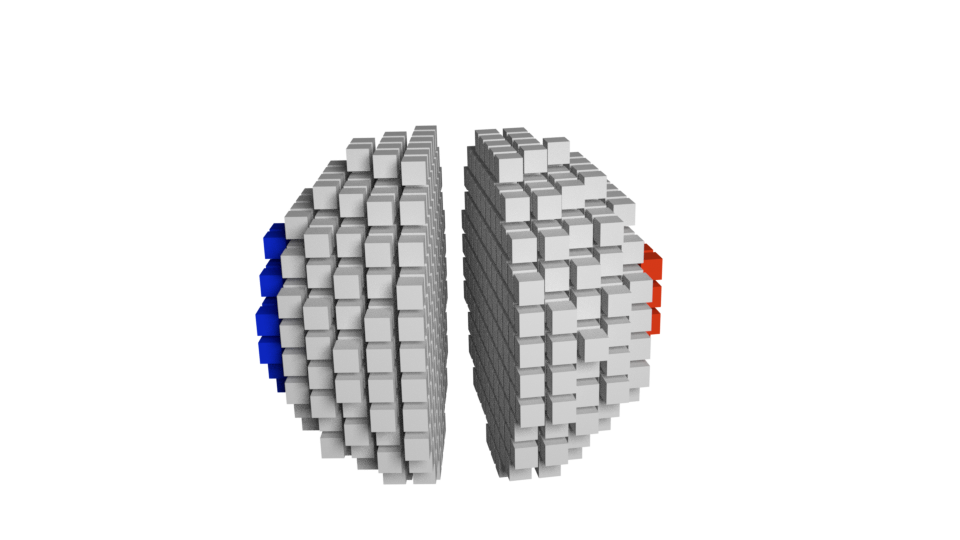
\includegraphics{media/pics/sliced_cube.png}
\caption{Numerical Grain}
\end{figure}

To simulate the spread of the bias potential areas inside the grain, a
technique called relaxation will be used. The general idea is to guess
an initial potential distribution, and then, based on the laws of
physics, iteratively correct this guess. The correction is done by
re-calculating each time the potential \(U_0\) of one center-``cube''
based on potential \(U_i\) and conductivity \(\sigma\) of the direct
neighbors. By doing this for each ``cube'', the potential distribution
will more and more apply to the physical solution. When approaching to
the solution, the overall changes in the potential of each cube will get
smaller and smaller. In an ideal case it will not change anymore. In
this case the potential of eachcube will be just as it should be to
fulfill the laws of physics. To understand how this process can be
supported by the means of modern matrix operations, I will shorty derive
how \(U_0\) is calculated from the surrounding \(U_i\). In a second step
matrix convolution will be used to solve the problem efficiently. First
we will need to combine Ohm's law and Kirchhoff's first law:
\begin{align}
R  = \frac{\Delta U}{I} = \frac{{\rho}*l}{A} and \sum_{i}I_i=0\\
\rightarrow \sum_{i}\frac{\Delta U_i}{R_i} = \sum_{i}\frac{U_0-U_i}{\rho_i}\frac{A}{l}=0\\
\rightarrow \sum_{i}\frac{U_0-U_i}{\rho_i}\frac{A}{l}=0\\
\rightarrow \sum_{i}\frac{U_0}{\rho_i}=\sum_{i}\frac{U_i}{\rho_i}\\
\rightarrow U_0\sum_{i}\frac{1}{\rho_i}=\sum_{i}\frac{U_i}{\rho_i}\\
\rightarrow U_0=\frac{\sum_{i}\frac{U_i}{\rho_i}}{\sum_{i}\frac{1}{\rho_i}}\\
\rightarrow U_0=\frac{\sum_{i}{U_i*\sigma_i}}{\sum_{i}{\sigma_i}}=\frac{\sum_{i}{U_i*q*n*\mu_n }}{\sum_{i}{q*n*\mu_n }}\\=\frac{q*\mu_n}{q*\mu_n} \frac{\sum_{i}{U_i*n_i}}{\sum_{i}{n_i}}=\frac{\sum_{i}{U_i*n_i}}{\sum_{i}{n_i}}\label{u_center}\tag{$U_0$ from $U_i$}\\
\end{align} With \(A\) the cube face area and \(l\) the distance between
the cube centers, which have no relevance when using a model where all
cubes are equal.

    To evaluate the each \(n_i\) at arbitrary points r inside the grain, one
additional step is needed. Due to the nature of the numerical solution
from the previous notebook we know the value of \(n\) only at specific
points. For values between those fix-points, an interpolation between
the neighbors can be used. Again, SciPy and Python offer here also a
easy to use and robust solution.
\texttt{from\ scipy\ import\ interpolate} adds the \texttt{interpolate}
module into the kernel. The \texttt{interp1d} function of this module is
described
(\href{https://docs.scipy.org/doc/scipy/reference/generated/scipy.interpolate.interp1d.htm}{here})
as follows: \textgreater Interpolate a 1-D function. \textgreater{}
\textgreater x and y are arrays of values used to approximate some
function f: y = f(x). This class returns a function whose call method
uses interpolation to find the value of new points.

Since the values of \(n\) and \(r\) exist already precalculated for
specific points in the Dataframe, the following function is used to
create the appropriate function for continuous values of r.

    \begin{tcolorbox}[breakable, size=fbox, boxrule=1pt, pad at break*=1mm,colback=cellbackground, colframe=cellborder]
\prompt{In}{incolor}{191}{\boxspacing}
\begin{Verbatim}[commandchars=\\\{\}]
\PY{k+kn}{from} \PY{n+nn}{scipy} \PY{k+kn}{import} \PY{n}{interpolate}

\PY{k}{def} \PY{n+nf}{get\PYZus{}interpolated\PYZus{}n\PYZus{}v}\PY{p}{(}\PY{n}{ser}\PY{p}{,}\PY{n}{grain}\PY{p}{)}\PY{p}{:}
    
    \PY{n}{v} \PY{o}{=} \PY{n}{ser}\PY{p}{[}\PY{l+s+s1}{\PYZsq{}}\PY{l+s+s1}{v}\PY{l+s+s1}{\PYZsq{}}\PY{p}{]}
    \PY{n}{r} \PY{o}{=} \PY{n}{ser}\PY{p}{[}\PY{l+s+s1}{\PYZsq{}}\PY{l+s+s1}{r}\PY{l+s+s1}{\PYZsq{}}\PY{p}{]}
    \PY{n}{n} \PY{o}{=} \PY{n}{ser}\PY{p}{[}\PY{l+s+s1}{\PYZsq{}}\PY{l+s+s1}{n}\PY{l+s+s1}{\PYZsq{}}\PY{p}{]}
    
    \PY{n}{r}\PY{p}{[}\PY{l+m+mi}{0}\PY{p}{]} \PY{o}{=} \PY{l+m+mi}{0}
    
    \PY{n}{n\PYZus{}int} \PY{o}{=} \PY{n}{interpolate}\PY{o}{.}\PY{n}{interp1d}\PY{p}{(}\PY{n}{r}\PY{o}{*}\PY{n}{grain}\PY{o}{.}\PY{n}{material}\PY{o}{.}\PY{n}{LD}\PY{p}{,} \PY{n}{n}\PY{p}{,} \PY{n}{kind}\PY{o}{=}\PY{l+s+s1}{\PYZsq{}}\PY{l+s+s1}{linear}\PY{l+s+s1}{\PYZsq{}}\PY{p}{)}
    \PY{n}{v\PYZus{}int} \PY{o}{=} \PY{n}{interpolate}\PY{o}{.}\PY{n}{interp1d}\PY{p}{(}\PY{n}{r}\PY{o}{*}\PY{n}{grain}\PY{o}{.}\PY{n}{material}\PY{o}{.}\PY{n}{LD}\PY{p}{,} \PY{n}{v}\PY{p}{,} \PY{n}{kind}\PY{o}{=}\PY{l+s+s1}{\PYZsq{}}\PY{l+s+s1}{linear}\PY{l+s+s1}{\PYZsq{}}\PY{p}{)}
    
    \PY{k}{return} \PY{n}{n\PYZus{}int}\PY{p}{,} \PY{n}{v\PYZus{}int}
\end{Verbatim}
\end{tcolorbox}

    As mentioned earlier, the positions of the applied potential will only
be the cubes on the far left and right, as indicated in the picture. By
arranging the bias voltage like this, the potential inside the grain
will have a rotational symmetry along the axis connecting the two poles.
The benefit of the resulting symmetry by using this simplification is to
be able to represent the potential inside the grain by a \(N\times N\)
Matrix, where \(N\) are the number of cubes inside the grain. Since
\(N\times N\) data structures are very common in modern application
fields like computer vision and image recognition, many algorithm
dealing with such data structures are available. First we create now the
data structure of the grain for further simulations. The \(N\times N\)
cubes will be represented by a \texttt{numpy} array.

    \begin{tcolorbox}[breakable, size=fbox, boxrule=1pt, pad at break*=1mm,colback=cellbackground, colframe=cellborder]
\prompt{In}{incolor}{192}{\boxspacing}
\begin{Verbatim}[commandchars=\\\{\}]
\PY{k}{def} \PY{n+nf}{pos\PYZus{}to\PYZus{}r\PYZus{}o}\PY{p}{(}\PY{n}{xi}\PY{p}{,}\PY{n}{yi}\PY{p}{,}\PY{n}{grain}\PY{p}{,} \PY{n}{d}\PY{p}{)}\PY{p}{:}
    \PY{l+s+sd}{\PYZsq{}\PYZsq{}\PYZsq{}}
\PY{l+s+sd}{    By passing the xi and yi indices, the grain and one array, the position (r)}
\PY{l+s+sd}{    inside the grain is return}
\PY{l+s+sd}{    \PYZsq{}\PYZsq{}\PYZsq{}}
    \PY{n}{dx} \PY{o}{=} \PY{l+m+mi}{2}\PY{o}{*}\PY{n}{grain}\PY{o}{.}\PY{n}{R}\PY{o}{/}\PY{n}{d}\PY{o}{.}\PY{n}{shape}\PY{p}{[}\PY{l+m+mi}{0}\PY{p}{]}
    \PY{n}{cx} \PY{o}{=} \PY{n}{d}\PY{o}{.}\PY{n}{shape}\PY{p}{[}\PY{l+m+mi}{0}\PY{p}{]}\PY{o}{/}\PY{o}{/}\PY{l+m+mi}{2}
    \PY{n}{cy} \PY{o}{=} \PY{n}{d}\PY{o}{.}\PY{n}{shape}\PY{p}{[}\PY{l+m+mi}{1}\PY{p}{]}\PY{o}{/}\PY{o}{/}\PY{l+m+mi}{2}
    \PY{n}{ri} \PY{o}{=} \PY{p}{(}\PY{p}{(}\PY{n}{xi}\PY{o}{\PYZhy{}}\PY{n}{cx}\PY{p}{)}\PY{o}{*}\PY{o}{*}\PY{l+m+mi}{2}\PY{o}{+}\PY{p}{(}\PY{n}{yi}\PY{o}{\PYZhy{}}\PY{n}{cy}\PY{p}{)}\PY{o}{*}\PY{o}{*}\PY{l+m+mi}{2}\PY{p}{)}\PY{o}{*}\PY{o}{*}\PY{l+m+mf}{0.5}
    \PY{k}{return}\PY{p}{(}\PY{n}{ri}\PY{o}{*}\PY{n}{dx}\PY{p}{)}





\PY{k}{def} \PY{n+nf}{initaliz\PYZus{}d\PYZus{}v}\PY{p}{(}\PY{n}{d\PYZus{}v}\PY{p}{,} \PY{n}{d\PYZus{}mask}\PY{p}{,} \PY{n}{v}\PY{p}{)}\PY{p}{:}
    \PY{n}{d\PYZus{}v}\PY{p}{[}\PY{p}{:}\PY{p}{,}\PY{l+m+mi}{1}\PY{p}{]} \PY{o}{=} \PY{o}{\PYZhy{}}\PY{n}{v}
    \PY{n}{d\PYZus{}v}\PY{p}{[}\PY{p}{:}\PY{p}{,}\PY{l+m+mi}{0}\PY{p}{]} \PY{o}{=} \PY{o}{\PYZhy{}}\PY{n}{v}
    \PY{n}{d\PYZus{}v}\PY{p}{[}\PY{p}{:}\PY{p}{,}\PY{o}{\PYZhy{}}\PY{l+m+mi}{2}\PY{p}{]} \PY{o}{=} \PY{o}{+}\PY{n}{v}
    \PY{n}{d\PYZus{}v}\PY{p}{[}\PY{p}{:}\PY{p}{,}\PY{o}{\PYZhy{}}\PY{l+m+mi}{1}\PY{p}{]} \PY{o}{=} \PY{o}{+}\PY{n}{v}
    \PY{n}{d\PYZus{}v} \PY{o}{=} \PY{n}{d\PYZus{}v}\PY{o}{*}\PY{n}{d\PYZus{}mask}
    \PY{k}{return} \PY{n}{d\PYZus{}v}



\PY{k}{def} \PY{n+nf}{pos\PYZus{}to\PYZus{}r}\PY{p}{(}\PY{n}{xi}\PY{p}{,}\PY{n}{yi}\PY{p}{,}\PY{n}{grain}\PY{p}{,} \PY{n}{cube\PYZus{}size}\PY{p}{,} \PY{n}{d}\PY{p}{)}\PY{p}{:}
    \PY{l+s+sd}{\PYZsq{}\PYZsq{}\PYZsq{}}
\PY{l+s+sd}{    By passing the xi and yi indices, the grain and one array, the position (r)}
\PY{l+s+sd}{    inside the grain is return}
\PY{l+s+sd}{    \PYZsq{}\PYZsq{}\PYZsq{}}
    
    
    \PY{n}{cx} \PY{o}{=} \PY{n}{d}\PY{o}{.}\PY{n}{shape}\PY{p}{[}\PY{l+m+mi}{0}\PY{p}{]}\PY{o}{/}\PY{o}{/}\PY{l+m+mi}{2}\PY{o}{+}\PY{l+m+mi}{1}\PY{o}{\PYZhy{}}\PY{l+m+mi}{1} \PY{c+c1}{\PYZsh{}find the center; length divided by two without rest; +1; \PYZhy{}1 since we start at 0}
    \PY{n}{cy} \PY{o}{=} \PY{n}{d}\PY{o}{.}\PY{n}{shape}\PY{p}{[}\PY{l+m+mi}{1}\PY{p}{]}\PY{o}{/}\PY{o}{/}\PY{l+m+mi}{2}\PY{o}{+}\PY{l+m+mi}{1}\PY{o}{\PYZhy{}}\PY{l+m+mi}{1}
    
    \PY{n}{ri} \PY{o}{=} \PY{p}{(}\PY{p}{(}\PY{p}{(}\PY{n}{xi}\PY{o}{\PYZhy{}}\PY{n}{cx}\PY{p}{)}\PY{p}{)}\PY{o}{*}\PY{o}{*}\PY{l+m+mi}{2}\PY{o}{+}\PY{p}{(}\PY{p}{(}\PY{n}{yi}\PY{o}{\PYZhy{}}\PY{n}{cy}\PY{p}{)}\PY{p}{)}\PY{o}{*}\PY{o}{*}\PY{l+m+mi}{2}\PY{p}{)}\PY{o}{*}\PY{o}{*}\PY{l+m+mf}{0.5}
    \PY{k}{if} \PY{k+kc}{False}\PY{p}{:}
        \PY{n}{rx} \PY{o}{=} \PY{o}{\PYZhy{}}\PY{n}{grain}\PY{o}{.}\PY{n}{R}\PY{o}{+}\PY{n}{xi}\PY{o}{*}\PY{n}{cube\PYZus{}size}\PY{c+c1}{\PYZsh{}+0.5*cube\PYZus{}size}
        \PY{n}{ry} \PY{o}{=} \PY{o}{\PYZhy{}}\PY{n}{grain}\PY{o}{.}\PY{n}{R}\PY{o}{+}\PY{n}{yi}\PY{o}{*}\PY{n}{cube\PYZus{}size}\PY{c+c1}{\PYZsh{}+0.5*cube\PYZus{}size}
    
        \PY{n}{r} \PY{o}{=} \PY{p}{(}\PY{n}{rx}\PY{o}{*}\PY{o}{*}\PY{l+m+mi}{2}\PY{o}{+}\PY{n}{ry}\PY{o}{*}\PY{o}{*}\PY{l+m+mi}{2}\PY{p}{)}\PY{o}{*}\PY{o}{*}\PY{l+m+mf}{0.5}
    \PY{k}{else}\PY{p}{:}
        \PY{n}{r} \PY{o}{=} \PY{p}{(}\PY{n}{ri}\PY{o}{*}\PY{n}{cube\PYZus{}size}\PY{p}{)}
    \PY{k}{return} \PY{n}{r}

\PY{k}{def} \PY{n+nf}{r\PYZus{}to\PYZus{}pos}\PY{p}{(}\PY{n}{r}\PY{p}{,} \PY{n}{grain}\PY{p}{,} \PY{n}{cube\PYZus{}size}\PY{p}{,} \PY{n}{d\PYZus{}v}\PY{p}{)}\PY{p}{:}
    \PY{n}{center} \PY{o}{=} \PY{n}{d\PYZus{}v}\PY{o}{.}\PY{n}{shape}\PY{p}{[}\PY{l+m+mi}{0}\PY{p}{]}\PY{o}{/}\PY{o}{/}\PY{l+m+mi}{2}
    \PY{k}{return} \PY{n+nb}{int}\PY{p}{(}\PY{n+nb}{round}\PY{p}{(}\PY{n}{r}\PY{o}{/}\PY{n}{cube\PYZus{}size}\PY{p}{)}\PY{p}{)}\PY{o}{+}\PY{n}{center}
    

\PY{k}{def} \PY{n+nf}{create\PYZus{}numerical\PYZus{}grain\PYZus{}matrix}\PY{p}{(} \PY{n}{grain}\PY{p}{,} \PY{n}{ser}\PY{p}{,}\PY{n}{cube\PYZus{}size}\PY{p}{)}\PY{p}{:}
    \PY{c+c1}{\PYZsh{}these functions are needed to calculate the value of n and}
    \PY{c+c1}{\PYZsh{}v at arbitrary positions}
    \PY{n}{n\PYZus{}int}\PY{p}{,} \PY{n}{v\PYZus{}int} \PY{o}{=} \PY{n}{get\PYZus{}interpolated\PYZus{}n\PYZus{}v}\PY{p}{(}\PY{n}{ser}\PY{p}{,} \PY{n}{grain}\PY{p}{)}
    \PY{n}{nx} \PY{o}{=} \PY{n}{ny} \PY{o}{=} \PY{l+m+mi}{1}\PY{o}{+}\PY{l+m+mi}{2}\PY{o}{*}\PY{n+nb}{int}\PY{p}{(}\PY{n+nb}{round}\PY{p}{(}\PY{p}{(}\PY{n}{grain}\PY{o}{.}\PY{n}{R}\PY{o}{/}\PY{n}{cube\PYZus{}size}\PY{p}{)}\PY{p}{)}\PY{p}{)}
    \PY{c+c1}{\PYZsh{}print(nx,ny)}

    \PY{c+c1}{\PYZsh{}initalize the data for the volatege (d\PYZus{}v) and conductivity (d\PYZus{}cond) with zeros}
    \PY{n}{d\PYZus{}v} \PY{o}{=} \PY{n}{np}\PY{o}{.}\PY{n}{zeros}\PY{p}{(}\PY{p}{(}\PY{n}{nx}\PY{p}{,}\PY{n}{ny}\PY{p}{)}\PY{p}{)}
    \PY{n}{d\PYZus{}cond} \PY{o}{=} \PY{n}{np}\PY{o}{.}\PY{n}{zeros}\PY{p}{(}\PY{p}{(}\PY{n}{nx}\PY{p}{,}\PY{n}{ny}\PY{p}{)}\PY{p}{)}
    
    \PY{c+c1}{\PYZsh{}an additional mask for values outside the grain will be created}
    \PY{n}{d\PYZus{}mask} \PY{o}{=} \PY{n}{np}\PY{o}{.}\PY{n}{zeros}\PY{p}{(}\PY{p}{(}\PY{n}{nx}\PY{p}{,}\PY{n}{ny}\PY{p}{)}\PY{p}{)}
    

    \PY{k}{for} \PY{n}{xi} \PY{o+ow}{in} \PY{n+nb}{range}\PY{p}{(}\PY{n}{d\PYZus{}cond}\PY{o}{.}\PY{n}{shape}\PY{p}{[}\PY{l+m+mi}{0}\PY{p}{]}\PY{p}{)}\PY{p}{:}
        \PY{k}{for} \PY{n}{yi} \PY{o+ow}{in} \PY{n+nb}{range}\PY{p}{(}\PY{n}{d\PYZus{}cond}\PY{o}{.}\PY{n}{shape}\PY{p}{[}\PY{l+m+mi}{1}\PY{p}{]}\PY{p}{)}\PY{p}{:}
            \PY{n}{r} \PY{o}{=} \PY{n+nb}{float}\PY{p}{(}\PY{n}{pos\PYZus{}to\PYZus{}r}\PY{p}{(}\PY{n}{xi}\PY{p}{,}\PY{n}{yi}\PY{p}{,}\PY{n}{grain}\PY{p}{,} \PY{n}{cube\PYZus{}size}\PY{p}{,} \PY{n}{d\PYZus{}v}\PY{p}{)}\PY{p}{)}
            \PY{k}{try}\PY{p}{:}
                \PY{c+c1}{\PYZsh{}if r is outside the grain, n\PYZus{}int(r) will fail and got the except part below}
                \PY{c+c1}{\PYZsh{} otherwise the conductivity will be saved in units of nb}
                
                \PY{n}{condu} \PY{o}{=} \PY{n}{n\PYZus{}int}\PY{p}{(}\PY{n}{r}\PY{p}{)}\PY{o}{/}\PY{n}{grain}\PY{o}{.}\PY{n}{material}\PY{o}{.}\PY{n}{nb}
                
                \PY{n}{d\PYZus{}cond}\PY{p}{[}\PY{n}{xi}\PY{p}{,} \PY{n}{yi}\PY{p}{]} \PY{o}{=} \PY{n}{condu}
                
                \PY{c+c1}{\PYZsh{}since this point is inside the grain, the mask is 1}
                \PY{n}{d\PYZus{}mask}\PY{p}{[}\PY{n}{xi}\PY{p}{,}\PY{n}{yi}\PY{p}{]} \PY{o}{=} \PY{l+m+mi}{1}

            \PY{k}{except} \PY{n+ne}{ValueError}\PY{p}{:}
                \PY{c+c1}{\PYZsh{}outside the grain}
                \PY{n}{d\PYZus{}cond}\PY{p}{[}\PY{n}{xi}\PY{p}{,} \PY{n}{yi}\PY{p}{]} \PY{o}{=} \PY{l+m+mi}{0}
                \PY{n}{d\PYZus{}mask}\PY{p}{[}\PY{n}{xi}\PY{p}{,}\PY{n}{yi}\PY{p}{]} \PY{o}{=} \PY{l+m+mi}{0}
    \PY{n}{d\PYZus{}v} \PY{o}{=} \PY{n}{initaliz\PYZus{}d\PYZus{}v}\PY{p}{(}\PY{n}{d\PYZus{}v}\PY{p}{,} \PY{n}{d\PYZus{}mask}\PY{p}{,} \PY{l+m+mi}{1000}\PY{p}{)}
    \PY{k}{return} \PY{n}{d\PYZus{}v}\PY{p}{,} \PY{n}{d\PYZus{}cond}\PY{p}{,} \PY{n}{d\PYZus{}mask}
\end{Verbatim}
\end{tcolorbox}

    \hypertarget{precalc-the-numerical-grains-for-all-conditions}{%
\subsection{Precalc the numerical grains for all
conditions}\label{precalc-the-numerical-grains-for-all-conditions}}

The grain data structure can now a represented graphically. For faster
interactive response, we will pre initialize all the grains for the data
available. Due to the similarity of the \(N\times N\) data structure to
common pictures, the function \texttt{imshow} is very handy to represent
the data.

    \begin{tcolorbox}[breakable, size=fbox, boxrule=1pt, pad at break*=1mm,colback=cellbackground, colframe=cellborder]
\prompt{In}{incolor}{193}{\boxspacing}
\begin{Verbatim}[commandchars=\\\{\}]
\PY{n}{d\PYZus{}cond\PYZus{}plots} \PY{o}{=} \PY{p}{[}\PY{p}{]}
\PY{k}{for} \PY{n}{i}\PY{p}{,} \PY{n}{ser} \PY{o+ow}{in} \PY{n}{calc\PYZus{}dF}\PY{o}{.}\PY{n}{iterrows}\PY{p}{(}\PY{p}{)}\PY{p}{:}
    \PY{n+nb}{print}\PY{p}{(}\PY{l+s+sa}{f}\PY{l+s+s1}{\PYZsq{}}\PY{l+s+s1}{Initalized }\PY{l+s+s1}{\PYZob{}}\PY{l+s+s1}{i+1\PYZcb{} of }\PY{l+s+s1}{\PYZob{}}\PY{l+s+s1}{len(calc\PYZus{}dF)\PYZcb{}.}\PY{l+s+s1}{\PYZsq{}}\PY{p}{,} \PY{n}{end}\PY{o}{=}\PY{l+s+s1}{\PYZsq{}}\PY{l+s+se}{\PYZbs{}r}\PY{l+s+s1}{\PYZsq{}}\PY{p}{,} \PY{n}{flush}\PY{o}{=}\PY{k+kc}{True}\PY{p}{)}
    \PY{n}{grain} \PY{o}{=} \PY{n}{create\PYZus{}grain\PYZus{}from\PYZus{}data}\PY{p}{(}\PY{n}{ser}\PY{p}{)}
    \PY{n}{d\PYZus{}v}\PY{p}{,} \PY{n}{d\PYZus{}cond}\PY{p}{,}\PY{n}{d\PYZus{}mask} \PY{o}{=} \PY{n}{create\PYZus{}numerical\PYZus{}grain\PYZus{}matrix}\PY{p}{(} \PY{n}{grain}\PY{p}{,} \PY{n}{ser}\PY{p}{,}\PY{n}{cube\PYZus{}size}\PY{o}{=}\PY{l+m+mf}{5e\PYZhy{}9}\PY{p}{)}
    \PY{n}{d\PYZus{}cond\PYZus{}plot} \PY{o}{=} \PY{n}{d\PYZus{}cond}\PY{o}{.}\PY{n}{copy}\PY{p}{(}\PY{p}{)}
    \PY{n}{d\PYZus{}cond\PYZus{}plot}\PY{p}{[}\PY{n}{np}\PY{o}{.}\PY{n}{where}\PY{p}{(}\PY{n}{d\PYZus{}mask}\PY{o}{==}\PY{l+m+mi}{0}\PY{p}{)}\PY{p}{]}\PY{o}{=}\PY{k+kc}{None}
    \PY{n}{d\PYZus{}cond\PYZus{}plots}\PY{o}{.}\PY{n}{append}\PY{p}{(}\PY{n}{d\PYZus{}cond\PYZus{}plot}\PY{p}{)}
\PY{n}{calc\PYZus{}dF}\PY{o}{.}\PY{n}{loc}\PY{p}{[}\PY{p}{:}\PY{p}{,} \PY{l+s+s1}{\PYZsq{}}\PY{l+s+s1}{d\PYZus{}cond}\PY{l+s+s1}{\PYZsq{}}\PY{p}{]} \PY{o}{=} \PY{n}{d\PYZus{}cond\PYZus{}plots}
\end{Verbatim}
\end{tcolorbox}

    \begin{Verbatim}[commandchars=\\\{\}]
Initalized 84 of 252.
    \end{Verbatim}

    \begin{Verbatim}[commandchars=\\\{\}]

        ---------------------------------------------------------------------------

        KeyboardInterrupt                         Traceback (most recent call last)

        <ipython-input-193-b21451ab0705> in <module>
          3     print(f'Initalized \{i+1\} of \{len(calc\_dF)\}.', end='\textbackslash{}r', flush=True)
          4     grain = create\_grain\_from\_data(ser)
    ----> 5     d\_v, d\_cond,d\_mask = create\_numerical\_grain\_matrix( grain, ser,cube\_size=5e-9)
          6     d\_cond\_plot = d\_cond.copy()
          7     d\_cond\_plot[np.where(d\_mask==0)]=None


        <ipython-input-192-0ddeaec12b0d> in create\_numerical\_grain\_matrix(grain, ser, cube\_size)
         71                 \# otherwise the conductivity will be saved in units of nb
         72 
    ---> 73                 condu = n\_int(r)/grain.material.nb
         74 
         75                 d\_cond[xi, yi] = condu


        /usr/lib/python3.8/site-packages/scipy/interpolate/polyint.py in \_\_call\_\_(self, x)
         77         """
         78         x, x\_shape = self.\_prepare\_x(x)
    ---> 79         y = self.\_evaluate(x)
         80         return self.\_finish\_y(y, x\_shape)
         81 


        /usr/lib/python3.8/site-packages/scipy/interpolate/interpolate.py in \_evaluate(self, x\_new)
        661         y\_new = self.\_call(self, x\_new)
        662         if not self.\_extrapolate:
    --> 663             below\_bounds, above\_bounds = self.\_check\_bounds(x\_new)
        664             if len(y\_new) > 0:
        665                 \# Note fill\_value must be broadcast up to the proper size


        /usr/lib/python3.8/site-packages/scipy/interpolate/interpolate.py in \_check\_bounds(self, x\_new)
        685         \# fall outside the range of x.  Otherwise, we return an array indicating
        686         \# which values are outside the boundary region.
    --> 687         below\_bounds = x\_new < self.x[0]
        688         above\_bounds = x\_new > self.x[-1]
        689 


        KeyboardInterrupt: 

    \end{Verbatim}

    \begin{tcolorbox}[breakable, size=fbox, boxrule=1pt, pad at break*=1mm,colback=cellbackground, colframe=cellborder]
\prompt{In}{incolor}{127}{\boxspacing}
\begin{Verbatim}[commandchars=\\\{\}]
\PY{n}{calc\PYZus{}dF}\PY{o}{.}\PY{n}{to\PYZus{}hdf}\PY{p}{(}\PY{l+s+s1}{\PYZsq{}}\PY{l+s+s1}{precalc\PYZus{}dF.h5}\PY{l+s+s1}{\PYZsq{}}\PY{p}{,}\PY{l+s+s1}{\PYZsq{}}\PY{l+s+s1}{raw}\PY{l+s+s1}{\PYZsq{}}\PY{p}{,} \PY{n}{mode}\PY{o}{=} \PY{l+s+s1}{\PYZsq{}}\PY{l+s+s1}{w}\PY{l+s+s1}{\PYZsq{}}\PY{p}{)}
\end{Verbatim}
\end{tcolorbox}

    \begin{Verbatim}[commandchars=\\\{\}]
/usr/lib/python3.8/site-packages/pandas/core/generic.py:2530:
PerformanceWarning:
your performance may suffer as PyTables will pickle object types that it cannot
map directly to c-types [inferred\_type->mixed,key->block1\_values] [items->['n',
'r', 'v', 'v\_dot', 'd\_cond']]

  pytables.to\_hdf(path\_or\_buf, key, self, **kwargs)
    \end{Verbatim}

    \begin{tcolorbox}[breakable, size=fbox, boxrule=1pt, pad at break*=1mm,colback=cellbackground, colframe=cellborder]
\prompt{In}{incolor}{128}{\boxspacing}
\begin{Verbatim}[commandchars=\\\{\}]
\PY{n}{calc\PYZus{}dF} \PY{o}{=} \PY{n}{pd}\PY{o}{.}\PY{n}{read\PYZus{}hdf}\PY{p}{(}\PY{l+s+s1}{\PYZsq{}}\PY{l+s+s1}{precalc\PYZus{}dF.h5}\PY{l+s+s1}{\PYZsq{}}\PY{p}{,}\PY{l+s+s1}{\PYZsq{}}\PY{l+s+s1}{raw}\PY{l+s+s1}{\PYZsq{}}\PY{p}{)}
\end{Verbatim}
\end{tcolorbox}

    \begin{tcolorbox}[breakable, size=fbox, boxrule=1pt, pad at break*=1mm,colback=cellbackground, colframe=cellborder]
\prompt{In}{incolor}{194}{\boxspacing}
\begin{Verbatim}[commandchars=\\\{\}]
\PY{o}{\PYZpc{}}\PY{k}{matplotlib} inline
\end{Verbatim}
\end{tcolorbox}

    \begin{tcolorbox}[breakable, size=fbox, boxrule=1pt, pad at break*=1mm,colback=cellbackground, colframe=cellborder]
\prompt{In}{incolor}{195}{\boxspacing}
\begin{Verbatim}[commandchars=\\\{\}]
\PY{k}{def} \PY{n+nf}{plot\PYZus{}grain\PYZus{}states}\PY{p}{(}\PY{n}{calc\PYZus{}dF\PYZus{}grainsize}\PY{p}{,} \PY{n}{vmax}\PY{o}{=}\PY{k+kc}{None}\PY{p}{,} \PY{n}{vmin}\PY{o}{=}\PY{k+kc}{None}\PY{p}{)}\PY{p}{:}
    \PY{n}{fig}\PY{p}{,} \PY{n}{axes} \PY{o}{=} \PY{n}{subplots}\PY{p}{(}\PY{l+m+mi}{3}\PY{p}{,}\PY{l+m+mi}{3}\PY{p}{,} \PY{n}{figsize} \PY{o}{=} \PY{p}{(}\PY{l+m+mi}{16}\PY{p}{,}\PY{l+m+mi}{9}\PY{p}{)}\PY{p}{)}
    
    \PY{n}{grain} \PY{o}{=} \PY{n}{create\PYZus{}grain\PYZus{}from\PYZus{}data}\PY{p}{(}\PY{n}{calc\PYZus{}dF\PYZus{}grainsize}\PY{p}{)}

    \PY{k}{for} \PY{n}{ax\PYZus{}i}\PY{p}{,} \PY{p}{(}\PY{n}{vinit}\PY{p}{,} \PY{n}{ser}\PY{p}{)} \PY{o+ow}{in} \PY{n+nb}{enumerate}\PY{p}{(}\PY{n}{calc\PYZus{}dF\PYZus{}grainsize}\PY{o}{.}\PY{n}{iterrows}\PY{p}{(}\PY{p}{)}\PY{p}{)}\PY{p}{:}
        \PY{n}{axe} \PY{o}{=} \PY{n}{fig}\PY{o}{.}\PY{n}{axes}\PY{p}{[}\PY{n}{ax\PYZus{}i}\PY{p}{]}
        
        \PY{n}{Einit\PYZus{}kT} \PY{o}{=} \PY{n}{ser}\PY{p}{[}\PY{l+s+s1}{\PYZsq{}}\PY{l+s+s1}{Einit\PYZus{}kT}\PY{l+s+s1}{\PYZsq{}}\PY{p}{]}

        \PY{n}{axe}\PY{o}{.}\PY{n}{set\PYZus{}title}\PY{p}{(}\PY{l+s+sa}{r}\PY{l+s+s1}{\PYZsq{}}\PY{l+s+s1}{\PYZdl{}E\PYZus{}}\PY{l+s+s1}{\PYZob{}}\PY{l+s+s1}{C\PYZus{}}\PY{l+s+si}{\PYZob{}Surface\PYZcb{}}\PY{l+s+s1}{\PYZcb{}=\PYZdl{}}\PY{l+s+s1}{\PYZsq{}}\PY{o}{+}\PY{l+s+sa}{f}\PY{l+s+s1}{\PYZsq{}}\PY{l+s+si}{\PYZob{}Einit\PYZus{}kT\PYZcb{}}\PY{l+s+s1}{kT}\PY{l+s+s1}{\PYZsq{}}\PY{p}{)}
        \PY{n}{axe}\PY{o}{.}\PY{n}{set\PYZus{}ylabel}\PY{p}{(}\PY{l+s+s1}{\PYZsq{}}\PY{l+s+s1}{x [nm]}\PY{l+s+s1}{\PYZsq{}}\PY{p}{)}
        \PY{n}{axe}\PY{o}{.}\PY{n}{set\PYZus{}xlabel}\PY{p}{(}\PY{l+s+s1}{\PYZsq{}}\PY{l+s+s1}{y [nm]}\PY{l+s+s1}{\PYZsq{}}\PY{p}{)}
        
        \PY{n}{d\PYZus{}cond\PYZus{}plot} \PY{o}{=} \PY{n}{calc\PYZus{}dF}\PY{o}{.}\PY{n}{loc}\PY{p}{[}\PY{n}{ser}\PY{o}{.}\PY{n}{name}\PY{p}{,} \PY{l+s+s1}{\PYZsq{}}\PY{l+s+s1}{d\PYZus{}cond}\PY{l+s+s1}{\PYZsq{}}\PY{p}{]}
        \PY{c+c1}{\PYZsh{}using axe.imshow to plot the data on the axe}
        \PY{n}{axe}\PY{o}{.}\PY{n}{grid}\PY{p}{(}\PY{n}{b}\PY{o}{=}\PY{k+kc}{True}\PY{p}{,} \PY{n}{zorder}\PY{o}{=}\PY{o}{\PYZhy{}}\PY{l+m+mi}{5}\PY{p}{)}
        \PY{n}{im} \PY{o}{=} \PY{n}{axe}\PY{o}{.}\PY{n}{imshow}\PY{p}{(}\PY{n}{np}\PY{o}{.}\PY{n}{log}\PY{p}{(}\PY{n}{d\PYZus{}cond\PYZus{}plot}\PY{p}{)}\PY{p}{,} \PY{n}{interpolation}\PY{o}{=}\PY{l+s+s1}{\PYZsq{}}\PY{l+s+s1}{bicubic}\PY{l+s+s1}{\PYZsq{}}\PY{p}{,}
                        \PY{n}{extent}\PY{o}{=}\PY{p}{(}\PY{o}{\PYZhy{}}\PY{n}{grain}\PY{o}{.}\PY{n}{R}\PY{o}{*}\PY{l+m+mf}{1e9}\PY{p}{,} \PY{n}{grain}\PY{o}{.}\PY{n}{R}\PY{o}{*}\PY{l+m+mf}{1e9}\PY{p}{,} \PY{o}{\PYZhy{}}\PY{n}{grain}\PY{o}{.}\PY{n}{R}\PY{o}{*}\PY{l+m+mf}{1e9}\PY{p}{,} \PY{n}{grain}\PY{o}{.}\PY{n}{R}\PY{o}{*}\PY{l+m+mf}{1e9}\PY{p}{)}\PY{p}{,}
                        \PY{n}{vmax}\PY{o}{=}\PY{n}{vmax}\PY{p}{,} \PY{n}{vmin}\PY{o}{=}\PY{n}{vmin}\PY{p}{,} \PY{n}{cmap}\PY{o}{=}\PY{l+s+s1}{\PYZsq{}}\PY{l+s+s1}{hot}\PY{l+s+s1}{\PYZsq{}}\PY{p}{,} \PY{n}{zorder}\PY{o}{=}\PY{l+m+mi}{2}\PY{p}{)}
        
    \PY{n}{fig}\PY{o}{.}\PY{n}{tight\PYZus{}layout}\PY{p}{(}\PY{p}{)}
    \PY{n}{fig}\PY{o}{.}\PY{n}{subplots\PYZus{}adjust}\PY{p}{(}\PY{n}{top}\PY{o}{=}\PY{l+m+mf}{0.9}\PY{p}{)}
    \PY{n}{ND} \PY{o}{=} \PY{n}{calc\PYZus{}dF\PYZus{}grainsize}\PY{p}{[}\PY{l+s+s1}{\PYZsq{}}\PY{l+s+s1}{ND}\PY{l+s+s1}{\PYZsq{}}\PY{p}{]}\PY{o}{.}\PY{n}{unique}\PY{p}{(}\PY{p}{)}\PY{p}{[}\PY{l+m+mi}{0}\PY{p}{]}
    \PY{n}{fig}\PY{o}{.}\PY{n}{suptitle}\PY{p}{(}\PY{l+s+sa}{f}\PY{l+s+s1}{\PYZsq{}}\PY{l+s+s1}{ND: }\PY{l+s+si}{\PYZob{}ND\PYZcb{}}\PY{l+s+s1}{\PYZsq{}}\PY{p}{,} \PY{n}{fontsize}\PY{o}{=}\PY{l+m+mi}{22}\PY{p}{)}
    


\PY{k}{def} \PY{n+nf}{plot\PYZus{}conductivity}\PY{p}{(}\PY{n}{GrainRadius}\PY{p}{,} \PY{n}{ND}\PY{o}{=}\PY{l+m+mf}{9e21}\PY{p}{)}\PY{p}{:}
    \PY{n}{R} \PY{o}{=} \PY{n}{GrainRadius}\PY{o}{/}\PY{l+m+mf}{1e9}
    \PY{n}{calc\PYZus{}dF\PYZus{}grainsize} \PY{o}{=} \PY{n}{calc\PYZus{}dF}\PY{o}{.}\PY{n}{groupby}\PY{p}{(}\PY{p}{[}\PY{l+s+s1}{\PYZsq{}}\PY{l+s+s1}{ND}\PY{l+s+s1}{\PYZsq{}}\PY{p}{,}\PY{l+s+s1}{\PYZsq{}}\PY{l+s+s1}{R}\PY{l+s+s1}{\PYZsq{}}\PY{p}{]}\PY{p}{)}\PY{o}{.}\PY{n}{get\PYZus{}group}\PY{p}{(}\PY{p}{(}\PY{n}{ND}\PY{p}{,}\PY{n}{R}\PY{p}{)}\PY{p}{)}
    \PY{n}{max\PYZus{}n} \PY{o}{=} \PY{n}{np}\PY{o}{.}\PY{n}{log}\PY{p}{(}\PY{n}{calc\PYZus{}dF\PYZus{}grainsize}\PY{p}{[}\PY{l+s+s1}{\PYZsq{}}\PY{l+s+s1}{d\PYZus{}cond}\PY{l+s+s1}{\PYZsq{}}\PY{p}{]}\PY{o}{.}\PY{n}{apply}\PY{p}{(}\PY{k}{lambda} \PY{n}{r}\PY{p}{:}\PY{n}{np}\PY{o}{.}\PY{n}{nanmax}\PY{p}{(}\PY{n}{r}\PY{p}{)}\PY{p}{)}\PY{p}{)}\PY{o}{.}\PY{n}{max}\PY{p}{(}\PY{p}{)}
    \PY{n}{min\PYZus{}n} \PY{o}{=} \PY{n}{np}\PY{o}{.}\PY{n}{log}\PY{p}{(}\PY{n}{calc\PYZus{}dF\PYZus{}grainsize}\PY{p}{[}\PY{l+s+s1}{\PYZsq{}}\PY{l+s+s1}{d\PYZus{}cond}\PY{l+s+s1}{\PYZsq{}}\PY{p}{]}\PY{o}{.}\PY{n}{apply}\PY{p}{(}\PY{k}{lambda} \PY{n}{r}\PY{p}{:}\PY{n}{np}\PY{o}{.}\PY{n}{nanmin}\PY{p}{(}\PY{n}{r}\PY{p}{)}\PY{p}{)}\PY{p}{)}\PY{o}{.}\PY{n}{min}\PY{p}{(}\PY{p}{)}
    
    \PY{n}{plot\PYZus{}grain\PYZus{}states}\PY{p}{(}\PY{n}{calc\PYZus{}dF\PYZus{}grainsize}\PY{p}{,} \PY{n}{vmax} \PY{o}{=} \PY{n}{max\PYZus{}n}\PY{p}{,} \PY{n}{vmin} \PY{o}{=} \PY{n}{min\PYZus{}n}\PY{p}{)}


\PY{n}{use\PYZus{}interactive\PYZus{}controls} \PY{o}{=} \PY{k+kc}{True}

\PY{k}{if} \PY{n}{use\PYZus{}interactive\PYZus{}controls}\PY{p}{:}
    \PY{k+kn}{from} \PY{n+nn}{ipywidgets} \PY{k+kn}{import} \PY{n}{interact}\PY{p}{,} \PY{n}{interactive}\PY{p}{,} \PY{n}{fixed}\PY{p}{,} \PY{n}{interact\PYZus{}manual}
    \PY{k+kn}{import} \PY{n+nn}{ipywidgets} \PY{k}{as} \PY{n+nn}{widgets}
    \PY{n}{grainsizes} \PY{o}{=} \PY{n+nb}{list}\PY{p}{(}\PY{n}{calc\PYZus{}dF}\PY{p}{[}\PY{l+s+s1}{\PYZsq{}}\PY{l+s+s1}{R}\PY{l+s+s1}{\PYZsq{}}\PY{p}{]}\PY{o}{.}\PY{n}{unique}\PY{p}{(}\PY{p}{)}\PY{p}{)}
    \PY{n}{interact}\PY{p}{(}\PY{n}{plot\PYZus{}conductivity}\PY{p}{,} \PY{n}{GrainRadius}\PY{o}{=}\PY{n}{np}\PY{o}{.}\PY{n}{array}\PY{p}{(}\PY{n}{grainsizes}\PY{p}{)}\PY{o}{*}\PY{l+m+mf}{1e9}\PY{p}{,}\PY{n}{ND}\PY{o}{=}\PY{n+nb}{list}\PY{p}{(}\PY{n}{calc\PYZus{}dF}\PY{o}{.}\PY{n}{groupby}\PY{p}{(}\PY{p}{[}\PY{l+s+s1}{\PYZsq{}}\PY{l+s+s1}{ND}\PY{l+s+s1}{\PYZsq{}}\PY{p}{]}\PY{p}{)}\PY{o}{.}\PY{n}{groups}\PY{o}{.}\PY{n}{keys}\PY{p}{(}\PY{p}{)}\PY{p}{)}\PY{p}{,} \PY{n}{text}\PY{o}{=}\PY{l+s+s1}{\PYZsq{}}\PY{l+s+s1}{Select a grainsize:}\PY{l+s+s1}{\PYZsq{}}\PY{p}{)}\PY{p}{;}
\PY{k}{else}\PY{p}{:}
    \PY{n}{GrainRadius} \PY{o}{=} \PY{l+m+mi}{200}
    
    \PY{k}{for} \PY{n}{ND} \PY{o+ow}{in} \PY{n+nb}{list}\PY{p}{(}\PY{n}{calc\PYZus{}dF}\PY{o}{.}\PY{n}{groupby}\PY{p}{(}\PY{p}{[}\PY{l+s+s1}{\PYZsq{}}\PY{l+s+s1}{ND}\PY{l+s+s1}{\PYZsq{}}\PY{p}{]}\PY{p}{)}\PY{o}{.}\PY{n}{groups}\PY{o}{.}\PY{n}{keys}\PY{p}{(}\PY{p}{)}\PY{p}{)}\PY{p}{:}
        \PY{n}{plot\PYZus{}conductivity}\PY{p}{(}\PY{n}{GrainRadius}\PY{p}{,} \PY{n}{ND}\PY{p}{)}
        
\end{Verbatim}
\end{tcolorbox}

    
    \begin{verbatim}
interactive(children=(Dropdown(description='GrainRadius', options=(50.0, 100.0, 200.0, 400.0), value=50.0), Dr…
    \end{verbatim}

    
    \hypertarget{relaxation}{%
\subsection{Relaxation}\label{relaxation}}

\hypertarget{concolute2d}{%
\subsubsection{Concolute2d:}\label{concolute2d}}

Equation (\(\ref{u_center}\)) is the basis of the relaxation process.
The potential at each cube will be recalculated according to:
\(U_0 = \frac{\sum_{i}{U_i*n_i}}{\sum_{i}{n_i}}\label{u_center}\). The
indices \(i\) stand for the direct neighbors of \(U_0\). The following
simple example should explain how \texttt{convolve2d} can be used to
solve our task. The function needs two parameters as inputs. The first
is the matrix itself, while the second is the description of the
convolution operation. In a very short description, this is What the
algorithm will do:

\begin{enumerate}
\def\labelenumi{\arabic{enumi}.}
\tightlist
\item
  goto on datapoint i\_x\_y
\item
  multiply the neighbors of i\_x\_y with the corresponding value of the
  second argument
\item
  sum up the results and save it a the position of the datapoint i\_x\_y
\item
  do this for all data points
\end{enumerate}

It would be out of the scope to dig deeper into the details of
convolutions, but this working a bit with the following example should
reveal the main concept.

    \begin{tcolorbox}[breakable, size=fbox, boxrule=1pt, pad at break*=1mm,colback=cellbackground, colframe=cellborder]
\prompt{In}{incolor}{196}{\boxspacing}
\begin{Verbatim}[commandchars=\\\{\}]
\PY{k+kn}{from} \PY{n+nn}{scipy} \PY{k+kn}{import} \PY{n}{signal}

\PY{n}{U} \PY{o}{=} \PY{n}{np}\PY{o}{.}\PY{n}{array}\PY{p}{(}\PY{p}{[}\PY{p}{[}\PY{l+m+mi}{1}\PY{p}{,}\PY{l+m+mi}{2}\PY{p}{,}\PY{l+m+mi}{3}\PY{p}{]}\PY{p}{,}\PY{p}{[}\PY{l+m+mi}{1}\PY{p}{,}\PY{l+m+mi}{2}\PY{p}{,}\PY{l+m+mi}{3}\PY{p}{]}\PY{p}{,}\PY{p}{[}\PY{l+m+mi}{1}\PY{p}{,}\PY{l+m+mi}{2}\PY{p}{,}\PY{l+m+mi}{3}\PY{p}{]}\PY{p}{]}\PY{p}{)}
\PY{n+nb}{print}\PY{p}{(}\PY{l+s+s1}{\PYZsq{}}\PY{l+s+s1}{U:}\PY{l+s+s1}{\PYZsq{}}\PY{p}{)}
\PY{n+nb}{print}\PY{p}{(}\PY{n}{U}\PY{p}{)}
\PY{n+nb}{print}\PY{p}{(}\PY{p}{)}

\PY{n}{n} \PY{o}{=} \PY{n}{np}\PY{o}{.}\PY{n}{array}\PY{p}{(}\PY{p}{[}\PY{p}{[}\PY{l+m+mi}{1}\PY{p}{,}\PY{l+m+mi}{1}\PY{p}{,}\PY{l+m+mi}{1}\PY{p}{]}\PY{p}{,}\PY{p}{[}\PY{l+m+mi}{10}\PY{p}{,}\PY{l+m+mi}{10}\PY{p}{,}\PY{l+m+mi}{10}\PY{p}{]}\PY{p}{,}\PY{p}{[}\PY{l+m+mi}{100}\PY{p}{,}\PY{l+m+mi}{100}\PY{p}{,}\PY{l+m+mi}{100}\PY{p}{]}\PY{p}{]}\PY{p}{)}
\PY{n+nb}{print}\PY{p}{(}\PY{l+s+s1}{\PYZsq{}}\PY{l+s+s1}{n:}\PY{l+s+s1}{\PYZsq{}}\PY{p}{)}
\PY{n+nb}{print}\PY{p}{(}\PY{n}{n}\PY{p}{)}
\PY{n+nb}{print}\PY{p}{(}\PY{p}{)}

\PY{n+nb}{print}\PY{p}{(}\PY{l+s+s1}{\PYZsq{}}\PY{l+s+s1}{U*n}\PY{l+s+s1}{\PYZsq{}}\PY{p}{)}
\PY{n+nb}{print}\PY{p}{(}\PY{n}{U}\PY{o}{*}\PY{n}{n}\PY{p}{)}
\PY{n+nb}{print}\PY{p}{(}\PY{p}{)}

\PY{n}{conv} \PY{o}{=} \PY{n}{np}\PY{o}{.}\PY{n}{array}\PY{p}{(}\PY{p}{[}\PY{p}{[}\PY{l+m+mi}{0}\PY{p}{,}\PY{l+m+mi}{1}\PY{p}{,}\PY{l+m+mi}{0}\PY{p}{]}\PY{p}{,}\PY{p}{[}\PY{l+m+mi}{1}\PY{p}{,}\PY{l+m+mi}{0}\PY{p}{,}\PY{l+m+mi}{1}\PY{p}{]}\PY{p}{,}\PY{p}{[}\PY{l+m+mi}{0}\PY{p}{,}\PY{l+m+mi}{1}\PY{p}{,}\PY{l+m+mi}{0}\PY{p}{]}\PY{p}{]}\PY{p}{)}
\PY{n+nb}{print}\PY{p}{(}\PY{l+s+s1}{\PYZsq{}}\PY{l+s+s1}{Conv}\PY{l+s+s1}{\PYZsq{}}\PY{p}{)}
\PY{n+nb}{print}\PY{p}{(}\PY{n}{conv}\PY{p}{)}
\PY{n+nb}{print}\PY{p}{(}\PY{p}{)}


\PY{n}{signal}\PY{o}{.}\PY{n}{convolve2d}\PY{p}{(}\PY{n}{U}\PY{o}{*}\PY{n}{n}\PY{p}{,} \PY{n}{conv}\PY{p}{,} \PY{n}{boundary}\PY{o}{=}\PY{l+s+s1}{\PYZsq{}}\PY{l+s+s1}{fill}\PY{l+s+s1}{\PYZsq{}}\PY{p}{,} \PY{n}{mode}\PY{o}{=}\PY{l+s+s1}{\PYZsq{}}\PY{l+s+s1}{same}\PY{l+s+s1}{\PYZsq{}}\PY{p}{,} \PY{n}{fillvalue}\PY{o}{=}\PY{l+m+mi}{0}\PY{p}{)}
\end{Verbatim}
\end{tcolorbox}

    \begin{Verbatim}[commandchars=\\\{\}]
U:
[[1 2 3]
 [1 2 3]
 [1 2 3]]

n:
[[  1   1   1]
 [ 10  10  10]
 [100 100 100]]

U*n
[[  1   2   3]
 [ 10  20  30]
 [100 200 300]]

Conv
[[0 1 0]
 [1 0 1]
 [0 1 0]]

    \end{Verbatim}

            \begin{tcolorbox}[breakable, size=fbox, boxrule=.5pt, pad at break*=1mm, opacityfill=0]
\prompt{Out}{outcolor}{196}{\boxspacing}
\begin{Verbatim}[commandchars=\\\{\}]
array([[ 12,  24,  32],
       [121, 242, 323],
       [210, 420, 230]])
\end{Verbatim}
\end{tcolorbox}
        
    In the example it can be shown, how this function is helpful for solving
the relaxation problem. For instance the sum over the direct neighbors
of the center is: \(10+2+30+200=242\), This is exact the value as return
by the function. The process of calculating the convoluted matrix is
done for the nominator and the denominator. After the division \(U_0\)
is obtained. Some additional steps as masking the potentials outside the
grain setting the bias again. If the potential down not change anymore,
the iterations can be stopped.

    \begin{tcolorbox}[breakable, size=fbox, boxrule=1pt, pad at break*=1mm,colback=cellbackground, colframe=cellborder]
\prompt{In}{incolor}{197}{\boxspacing}
\begin{Verbatim}[commandchars=\\\{\}]
\PY{k+kn}{from} \PY{n+nn}{scipy} \PY{k+kn}{import} \PY{n}{signal}


\PY{k}{def} \PY{n+nf}{solve\PYZus{}relaxation}\PY{p}{(}\PY{n}{d\PYZus{}v}\PY{p}{,} \PY{n}{d\PYZus{}cond}\PY{p}{,} \PY{n}{d\PYZus{}mask}\PY{p}{,} \PY{n}{n} \PY{o}{=} \PY{l+m+mi}{10000000}\PY{p}{)}\PY{p}{:}
    \PY{n}{res\PYZus{}new} \PY{o}{=} \PY{l+m+mi}{1000}
    \PY{c+c1}{\PYZsh{}shortly disable the error when dividing by zero (denominator)}
    \PY{n}{old\PYZus{}settings} \PY{o}{=} \PY{n}{np}\PY{o}{.}\PY{n}{seterr}\PY{p}{(}\PY{p}{)}
    \PY{n}{np}\PY{o}{.}\PY{n}{seterr}\PY{p}{(}\PY{n}{divide}\PY{o}{=}\PY{l+s+s1}{\PYZsq{}}\PY{l+s+s1}{ignore}\PY{l+s+s1}{\PYZsq{}}\PY{p}{,} \PY{n}{invalid}\PY{o}{=}\PY{l+s+s1}{\PYZsq{}}\PY{l+s+s1}{ignore}\PY{l+s+s1}{\PYZsq{}}\PY{p}{)}
    \PY{n}{conv} \PY{o}{=} \PY{p}{[}\PY{p}{[}\PY{l+m+mi}{0}\PY{p}{,}\PY{l+m+mi}{1}\PY{p}{,}\PY{l+m+mi}{0}\PY{p}{]}\PY{p}{,}\PY{p}{[}\PY{l+m+mi}{1}\PY{p}{,}\PY{l+m+mi}{0}\PY{p}{,}\PY{l+m+mi}{1}\PY{p}{]}\PY{p}{,}\PY{p}{[}\PY{l+m+mi}{0}\PY{p}{,}\PY{l+m+mi}{1}\PY{p}{,}\PY{l+m+mi}{0}\PY{p}{]}\PY{p}{]}
    \PY{n}{denominator} \PY{o}{=} \PY{n}{signal}\PY{o}{.}\PY{n}{convolve2d}\PY{p}{(}\PY{n}{d\PYZus{}cond}\PY{p}{,} \PY{n}{conv}\PY{p}{,} \PY{n}{boundary}\PY{o}{=}\PY{l+s+s1}{\PYZsq{}}\PY{l+s+s1}{fill}\PY{l+s+s1}{\PYZsq{}}\PY{p}{,}
                                \PY{n}{mode}\PY{o}{=}\PY{l+s+s1}{\PYZsq{}}\PY{l+s+s1}{same}\PY{l+s+s1}{\PYZsq{}}\PY{p}{,} \PY{n}{fillvalue}\PY{o}{=}\PY{l+m+mi}{0}\PY{p}{)}
    \PY{k}{for} \PY{n}{i} \PY{o+ow}{in} \PY{n+nb}{range}\PY{p}{(}\PY{n}{n}\PY{p}{)}\PY{p}{:}

        
        \PY{n}{numerator} \PY{o}{=} \PY{n}{signal}\PY{o}{.}\PY{n}{convolve2d}\PY{p}{(}\PY{n}{d\PYZus{}v}\PY{o}{*}\PY{n}{d\PYZus{}cond}\PY{p}{,} \PY{n}{conv}\PY{p}{,} \PY{n}{boundary}\PY{o}{=}\PY{l+s+s1}{\PYZsq{}}\PY{l+s+s1}{fill}\PY{l+s+s1}{\PYZsq{}}\PY{p}{,}
                                      \PY{n}{mode}\PY{o}{=}\PY{l+s+s1}{\PYZsq{}}\PY{l+s+s1}{same}\PY{l+s+s1}{\PYZsq{}}\PY{p}{,} \PY{n}{fillvalue}\PY{o}{=}\PY{l+m+mi}{0}\PY{p}{)}

        \PY{n}{d\PYZus{}v\PYZus{}new} \PY{o}{=} \PY{p}{(}\PY{n}{numerator}\PY{o}{/}\PY{n}{denominator}\PY{p}{)}\PY{o}{*}\PY{n}{d\PYZus{}mask}
        \PY{n}{d\PYZus{}v\PYZus{}new} \PY{o}{=} \PY{n}{np}\PY{o}{.}\PY{n}{nan\PYZus{}to\PYZus{}num}\PY{p}{(}\PY{n}{d\PYZus{}v\PYZus{}new}\PY{p}{,}\PY{l+m+mi}{0}\PY{p}{)}

        \PY{n}{d\PYZus{}v\PYZus{}prev} \PY{o}{=} \PY{n}{d\PYZus{}v}\PY{o}{.}\PY{n}{copy}\PY{p}{(}\PY{p}{)}
        

        
        \PY{n}{d\PYZus{}v} \PY{o}{=} \PY{n}{d\PYZus{}v\PYZus{}new}\PY{o}{.}\PY{n}{copy}\PY{p}{(}\PY{p}{)}
        \PY{n}{d\PYZus{}v} \PY{o}{=} \PY{n}{initaliz\PYZus{}d\PYZus{}v}\PY{p}{(}\PY{n}{d\PYZus{}v}\PY{p}{,} \PY{n}{d\PYZus{}mask}\PY{p}{,} \PY{l+m+mi}{1000}\PY{p}{)}

        \PY{n}{res\PYZus{}pre} \PY{o}{=} \PY{n}{res\PYZus{}new}
        \PY{n}{res\PYZus{}new} \PY{o}{=} \PY{n}{np}\PY{o}{.}\PY{n}{abs}\PY{p}{(}\PY{n}{np}\PY{o}{.}\PY{n}{sum}\PY{p}{(}\PY{n}{d\PYZus{}v\PYZus{}prev}\PY{o}{\PYZhy{}}\PY{n}{d\PYZus{}v}\PY{p}{)}\PY{p}{)}

        \PY{k}{if} \PY{n}{i}\PY{o}{\PYZpc{}}\PY{k}{10000}==1:
            \PY{c+c1}{\PYZsh{}print(res\PYZus{}pre,res\PYZus{}new)}
            
            \PY{k}{if} \PY{p}{(}\PY{p}{(}\PY{n}{res\PYZus{}pre} \PY{o}{\PYZhy{}} \PY{n}{res\PYZus{}new}\PY{p}{)}\PY{o}{==}\PY{l+m+mi}{0}\PY{p}{)} \PY{o+ow}{and} \PY{p}{(}\PY{n}{i}\PY{o}{\PYZgt{}}\PY{l+m+mi}{40000}\PY{p}{)}\PY{p}{:}
                \PY{k}{break}
    \PY{c+c1}{\PYZsh{}setting back the defaults}
    \PY{n}{np}\PY{o}{.}\PY{n}{seterr}\PY{p}{(}\PY{o}{*}\PY{o}{*}\PY{n}{old\PYZus{}settings}\PY{p}{)}
    \PY{k}{return} \PY{n}{d\PYZus{}v}\PY{p}{,} \PY{n}{d\PYZus{}cond}\PY{p}{,} \PY{n}{d\PYZus{}mask}
\end{Verbatim}
\end{tcolorbox}

    When the potentials inside the grain is solved with the relaxation
algorithm, it is time to calculate the total resistance of the grain.
Since the relaxation was solved by applying a ``virtual'' potential
(\(\Phi\)) to the grain, the total resistance \(\Omega\) could be
calculated by Ohm's low: \(\Omega = \frac{\Delta \Phi}{Current}\), where
\(\Delta \Phi = V\) is the potential difference.

Therefore only the current trough the grain needs to be calculated. This
can be done by calculating the total current passing the slice in the
center of the grain. \begin{align}
j=\underset{A\rightarrow0}{lim}\frac{I_{A}}{A}=\underset{d\rightarrow0}{lim}\frac{I_{A}}{d*d}=\sigma E \\
E = \frac{V}{d}=\frac{\Delta \Phi}{d} \\
I_A = \sigma*V*d
\end{align} which will be the current going through one cube

    \begin{tcolorbox}[breakable, size=fbox, boxrule=1pt, pad at break*=1mm,colback=cellbackground, colframe=cellborder]
\prompt{In}{incolor}{198}{\boxspacing}
\begin{Verbatim}[commandchars=\\\{\}]
\PY{k}{def} \PY{n+nf}{calc\PYZus{}current\PYZus{}center}\PY{p}{(}\PY{n}{d\PYZus{}v}\PY{p}{,} \PY{n}{d\PYZus{}cond}\PY{p}{,} \PY{n}{d\PYZus{}mask}\PY{p}{,} \PY{n}{cube\PYZus{}size}\PY{p}{,} \PY{n}{grain}\PY{p}{)}\PY{p}{:}
    \PY{c+c1}{\PYZsh{}center\PYZus{}pos = d\PYZus{}v.shape[0]//2}
    \PY{c+c1}{\PYZsh{}center\PYZus{}pos = 20}
    \PY{n}{center\PYZus{}pos} \PY{o}{=} \PY{n}{r\PYZus{}to\PYZus{}pos}\PY{p}{(}\PY{l+m+mi}{0}\PY{p}{,} \PY{n}{grain}\PY{p}{,} \PY{n}{cube\PYZus{}size}\PY{p}{,} \PY{n}{d\PYZus{}v}\PY{p}{)}
    \PY{n}{center\PYZus{}current} \PY{o}{=} \PY{p}{(}\PY{n}{d\PYZus{}v}\PY{p}{[}\PY{p}{:}\PY{p}{,}\PY{n}{center\PYZus{}pos}\PY{o}{+}\PY{l+m+mi}{1}\PY{p}{]}\PY{o}{\PYZhy{}}\PY{n}{d\PYZus{}v}\PY{p}{[}\PY{p}{:}\PY{p}{,}\PY{n}{center\PYZus{}pos}\PY{o}{\PYZhy{}}\PY{l+m+mi}{1}\PY{p}{]}\PY{p}{)}\PY{o}{*}\PY{n}{d\PYZus{}cond}\PY{p}{[}\PY{p}{:}\PY{p}{,}\PY{n}{center\PYZus{}pos}\PY{p}{]}
    
    \PY{n}{r} \PY{o}{=} \PY{n}{np}\PY{o}{.}\PY{n}{array}\PY{p}{(}\PY{p}{[}\PY{n+nb}{float}\PY{p}{(}\PY{n}{pos\PYZus{}to\PYZus{}r}\PY{p}{(}\PY{n}{xi}\PY{p}{,}\PY{n}{center\PYZus{}pos}\PY{p}{,}\PY{n}{grain}\PY{p}{,} \PY{n}{cube\PYZus{}size}\PY{p}{,} \PY{n}{d\PYZus{}v}\PY{p}{)}\PY{p}{)} \PY{k}{for} \PY{n}{xi} \PY{o+ow}{in} \PY{n+nb}{range}\PY{p}{(}\PY{n+nb}{len}\PY{p}{(}\PY{n}{center\PYZus{}current}\PY{p}{)}\PY{p}{)}\PY{p}{]}\PY{p}{)}
    
    \PY{n}{center\PYZus{}current\PYZus{}tot} \PY{o}{=} \PY{n}{np}\PY{o}{.}\PY{n}{sum}\PY{p}{(}\PY{n}{center\PYZus{}current}\PY{o}{*}\PY{l+m+mi}{2}\PY{o}{*}\PY{n}{pi}\PY{o}{*}\PY{n}{r}\PY{p}{)}
    \PY{k}{return} \PY{n}{center\PYZus{}current\PYZus{}tot}\PY{p}{,} \PY{n}{center\PYZus{}current}\PY{p}{,} \PY{n}{r}
\end{Verbatim}
\end{tcolorbox}

    \begin{tcolorbox}[breakable, size=fbox, boxrule=1pt, pad at break*=1mm,colback=cellbackground, colframe=cellborder]
\prompt{In}{incolor}{199}{\boxspacing}
\begin{Verbatim}[commandchars=\\\{\}]
\PY{n}{calc\PYZus{}dF}\PY{p}{[}\PY{l+s+s1}{\PYZsq{}}\PY{l+s+s1}{current}\PY{l+s+s1}{\PYZsq{}}\PY{p}{]} \PY{o}{=} \PY{k+kc}{None}
\end{Verbatim}
\end{tcolorbox}

    \hypertarget{see-how-a-single-solution-evolves}{%
\section{See how a single solution
evolves}\label{see-how-a-single-solution-evolves}}

The interactive environment of Jupyter will be needed here. The
following command activates it. (For some unknown reasons, you might
need to execute this command 2-3 times to get activated)

    \begin{tcolorbox}[breakable, size=fbox, boxrule=1pt, pad at break*=1mm,colback=cellbackground, colframe=cellborder]
\prompt{In}{incolor}{200}{\boxspacing}
\begin{Verbatim}[commandchars=\\\{\}]
\PY{o}{\PYZpc{}}\PY{k}{matplotlib} inline
\end{Verbatim}
\end{tcolorbox}

    \begin{tcolorbox}[breakable, size=fbox, boxrule=1pt, pad at break*=1mm,colback=cellbackground, colframe=cellborder]
\prompt{In}{incolor}{18}{\boxspacing}
\begin{Verbatim}[commandchars=\\\{\}]
\PY{k+kn}{import} \PY{n+nn}{matplotlib}\PY{n+nn}{.}\PY{n+nn}{animation} \PY{k}{as} \PY{n+nn}{animation}

\PY{n}{c\PYZus{}dF} \PY{o}{=} \PY{n}{calc\PYZus{}dF}\PY{o}{.}\PY{n}{copy}\PY{p}{(}\PY{p}{)}
\PY{n}{cube\PYZus{}size} \PY{o}{=} \PY{l+m+mf}{5e\PYZhy{}9}
\PY{n}{c\PYZus{}dF}\PY{p}{[}\PY{l+s+s1}{\PYZsq{}}\PY{l+s+s1}{cube\PYZus{}size}\PY{l+s+s1}{\PYZsq{}}\PY{p}{]} \PY{o}{=} \PY{n}{cube\PYZus{}size}
\PY{n}{ser} \PY{o}{=}\PY{n}{c\PYZus{}dF}\PY{p}{[}\PY{p}{(}\PY{n}{c\PYZus{}dF}\PY{p}{[}\PY{l+s+s1}{\PYZsq{}}\PY{l+s+s1}{R}\PY{l+s+s1}{\PYZsq{}}\PY{p}{]}\PY{o}{==}\PY{l+m+mf}{400e\PYZhy{}9}\PY{p}{)} \PY{o}{\PYZam{}} \PY{p}{(}\PY{n}{c\PYZus{}dF}\PY{p}{[}\PY{l+s+s1}{\PYZsq{}}\PY{l+s+s1}{Einit\PYZus{}kT}\PY{l+s+s1}{\PYZsq{}}\PY{p}{]}\PY{o}{==}\PY{o}{\PYZhy{}}\PY{l+m+mi}{8}\PY{p}{)} \PY{o}{\PYZam{}} \PY{p}{(}\PY{n}{c\PYZus{}dF}\PY{p}{[}\PY{l+s+s1}{\PYZsq{}}\PY{l+s+s1}{ND}\PY{l+s+s1}{\PYZsq{}}\PY{p}{]}\PY{o}{==}\PY{l+m+mf}{9e21}\PY{p}{)}\PY{p}{]}\PY{o}{.}\PY{n}{iloc}\PY{p}{[}\PY{l+m+mi}{0}\PY{p}{]}

\PY{n}{vinit} \PY{o}{=} \PY{n}{ser}\PY{o}{.}\PY{n}{name}
\PY{n}{grain} \PY{o}{=} \PY{n}{create\PYZus{}grain\PYZus{}from\PYZus{}data}\PY{p}{(}\PY{n}{ser}\PY{p}{)}

\PY{k}{if} \PY{n}{cube\PYZus{}size}\PY{o}{==}\PY{l+s+s1}{\PYZsq{}}\PY{l+s+s1}{LD}\PY{l+s+s1}{\PYZsq{}}\PY{p}{:}
    \PY{n}{cube\PYZus{}size\PYZus{}value} \PY{o}{=} \PY{n}{grain}\PY{o}{.}\PY{n}{material}\PY{o}{.}\PY{n}{LD}\PY{o}{/}\PY{l+m+mi}{2}
\PY{k}{else}\PY{p}{:}
    \PY{n}{cube\PYZus{}size\PYZus{}value} \PY{o}{=} \PY{n}{cube\PYZus{}size}

\PY{n}{d\PYZus{}v}\PY{p}{,} \PY{n}{d\PYZus{}cond}\PY{p}{,} \PY{n}{d\PYZus{}mask} \PY{o}{=} \PY{n}{create\PYZus{}numerical\PYZus{}grain\PYZus{}matrix}\PY{p}{(} \PY{n}{grain}\PY{p}{,} \PY{n}{ser}\PY{p}{,}\PY{n}{cube\PYZus{}size}\PY{o}{=}\PY{n}{cube\PYZus{}size\PYZus{}value}\PY{p}{)}
\PY{n}{ns} \PY{o}{=} \PY{l+m+mi}{0}
\PY{k}{def} \PY{n+nf}{update}\PY{p}{(}\PY{n}{frame}\PY{p}{)}\PY{p}{:}
    \PY{n}{axe}\PY{o}{.}\PY{n}{clear}\PY{p}{(}\PY{p}{)}
    \PY{n}{axe\PYZus{}v}\PY{o}{.}\PY{n}{clear}\PY{p}{(}\PY{p}{)}
    \PY{n}{n} \PY{o}{=} \PY{l+m+mi}{100}
    \PY{k}{global} \PY{n}{d\PYZus{}v}
    \PY{k}{global} \PY{n}{ns}
    \PY{n}{ns}\PY{o}{+}\PY{o}{=}\PY{n}{n}
    \PY{n}{axe}\PY{o}{.}\PY{n}{set\PYZus{}title}\PY{p}{(}\PY{l+s+sa}{f}\PY{l+s+s1}{\PYZsq{}}\PY{l+s+s1}{Number relaxation interations: }\PY{l+s+si}{\PYZob{}ns\PYZcb{}}\PY{l+s+s1}{\PYZsq{}}\PY{p}{)}
    \PY{n}{axe\PYZus{}v}\PY{o}{.}\PY{n}{set\PYZus{}title}\PY{p}{(}\PY{l+s+s1}{\PYZsq{}}\PY{l+s+s1}{Potential inside from middle\PYZhy{}left to middle\PYZhy{}right}\PY{l+s+s1}{\PYZsq{}}\PY{p}{)}
    
    \PY{n}{d\PYZus{}v}\PY{p}{,} \PY{n}{\PYZus{}}\PY{p}{,} \PY{n}{\PYZus{}} \PY{o}{=} \PY{n}{solve\PYZus{}relaxation}\PY{p}{(}\PY{n}{d\PYZus{}v} \PY{o}{=} \PY{n}{d\PYZus{}v} \PY{p}{,} \PY{n}{d\PYZus{}cond}\PY{o}{=}\PY{n}{d\PYZus{}cond}\PY{p}{,} \PY{n}{d\PYZus{}mask}\PY{o}{=}\PY{n}{d\PYZus{}mask}\PY{p}{,} \PY{n}{n}\PY{o}{=}\PY{n}{n}\PY{p}{)}
    \PY{n}{d\PYZus{}v\PYZus{}plot} \PY{o}{=} \PY{n}{d\PYZus{}v}\PY{o}{.}\PY{n}{copy}\PY{p}{(}\PY{p}{)}
    \PY{n}{d\PYZus{}v\PYZus{}plot}\PY{p}{[}\PY{n}{np}\PY{o}{.}\PY{n}{where}\PY{p}{(}\PY{n}{d\PYZus{}mask}\PY{o}{==}\PY{l+m+mi}{0}\PY{p}{)}\PY{p}{]}\PY{o}{=}\PY{k+kc}{None}
    \PY{n}{img} \PY{o}{=} \PY{n}{axe}\PY{o}{.}\PY{n}{imshow}\PY{p}{(}\PY{n}{d\PYZus{}v\PYZus{}plot}\PY{p}{,}\PY{n}{interpolation}\PY{o}{=}\PY{l+s+s1}{\PYZsq{}}\PY{l+s+s1}{bicubic}\PY{l+s+s1}{\PYZsq{}}\PY{p}{,}\PY{p}{)}
    
    
    \PY{n}{axe\PYZus{}v}\PY{o}{.}\PY{n}{plot}\PY{p}{(}\PY{n}{d\PYZus{}v}\PY{p}{[}\PY{n}{r\PYZus{}to\PYZus{}pos}\PY{p}{(}\PY{l+m+mi}{0}\PY{p}{,}\PY{n}{grain}\PY{p}{,} \PY{n}{cube\PYZus{}size}\PY{p}{,} \PY{n}{d\PYZus{}v}\PY{p}{)}\PY{p}{,}\PY{p}{:}\PY{p}{]}\PY{p}{)}
    
    \PY{c+c1}{\PYZsh{}plot\PYZus{}grad(axe\PYZus{}g, axe\PYZus{}c, d\PYZus{}v=d\PYZus{}v, d\PYZus{}mask=d\PYZus{}mask)}
    
    \PY{k}{return} \PY{n}{img}


\PY{n}{fig}\PY{p}{,} \PY{n}{axes} \PY{o}{=} \PY{n}{subplots}\PY{p}{(}\PY{l+m+mi}{1}\PY{p}{,}\PY{l+m+mi}{2}\PY{p}{,} \PY{n}{figsize} \PY{o}{=} \PY{p}{(}\PY{l+m+mi}{16}\PY{p}{,}\PY{l+m+mi}{9}\PY{p}{)}\PY{p}{)}
\PY{k+kn}{import} \PY{n+nn}{matplotlib}\PY{n+nn}{.}\PY{n+nn}{pyplot} \PY{k}{as} \PY{n+nn}{plt}
\PY{k+kn}{from} \PY{n+nn}{matplotlib}\PY{n+nn}{.}\PY{n+nn}{animation} \PY{k+kn}{import} \PY{n}{FuncAnimation}

\PY{n}{axe} \PY{o}{=} \PY{n}{axes}\PY{p}{[}\PY{l+m+mi}{0}\PY{p}{]}

\PY{n}{img} \PY{o}{=} \PY{n}{axe}\PY{o}{.}\PY{n}{imshow}\PY{p}{(}\PY{n}{d\PYZus{}v}\PY{p}{)}
\PY{n}{cb} \PY{o}{=} \PY{n}{colorbar}\PY{p}{(}\PY{n}{img}\PY{p}{,} \PY{n}{ax} \PY{o}{=} \PY{n}{axe}\PY{p}{)}
\PY{n}{cb}\PY{o}{.}\PY{n}{ax}\PY{o}{.}\PY{n}{set\PYZus{}ylabel}\PY{p}{(}\PY{l+s+s1}{\PYZsq{}}\PY{l+s+s1}{Volage [V]}\PY{l+s+s1}{\PYZsq{}}\PY{p}{)}

\PY{n}{axe\PYZus{}v} \PY{o}{=} \PY{n}{axes}\PY{p}{[}\PY{l+m+mi}{1}\PY{p}{]}


\PY{n}{ani} \PY{o}{=} \PY{n}{FuncAnimation}\PY{p}{(}\PY{n}{fig}\PY{p}{,} \PY{n}{update}\PY{p}{,} \PY{n}{frames} \PY{o}{=} \PY{n+nb}{list}\PY{p}{(}\PY{n+nb}{range}\PY{p}{(}\PY{l+m+mi}{100}\PY{p}{)}\PY{p}{)}\PY{p}{,} \PY{n}{interval}\PY{o}{=}\PY{l+m+mi}{10}\PY{p}{,}\PY{n}{blit}\PY{o}{=}\PY{k+kc}{False}\PY{p}{,} \PY{n}{repeat} \PY{o}{=} \PY{k+kc}{False}\PY{p}{)}

\PY{c+c1}{\PYZsh{} Set up formatting for the movie files}
\PY{n}{Writer} \PY{o}{=} \PY{n}{animation}\PY{o}{.}\PY{n}{writers}\PY{p}{[}\PY{l+s+s1}{\PYZsq{}}\PY{l+s+s1}{ffmpeg}\PY{l+s+s1}{\PYZsq{}}\PY{p}{]}
\PY{n}{writer} \PY{o}{=} \PY{n}{Writer}\PY{p}{(}\PY{n}{fps}\PY{o}{=}\PY{l+m+mi}{15}\PY{p}{,} \PY{n}{metadata}\PY{o}{=}\PY{n+nb}{dict}\PY{p}{(}\PY{n}{artist}\PY{o}{=}\PY{l+s+s1}{\PYZsq{}}\PY{l+s+s1}{Me}\PY{l+s+s1}{\PYZsq{}}\PY{p}{)}\PY{p}{,} \PY{n}{bitrate}\PY{o}{=}\PY{l+m+mi}{1800}\PY{p}{)}
\PY{n}{ani}\PY{o}{.}\PY{n}{save}\PY{p}{(}\PY{l+s+s1}{\PYZsq{}}\PY{l+s+s1}{im.mp4}\PY{l+s+s1}{\PYZsq{}}\PY{p}{,} \PY{n}{writer}\PY{o}{=}\PY{n}{writer}\PY{p}{)}

\PY{n}{plt}\PY{o}{.}\PY{n}{show}\PY{p}{(}\PY{p}{)}
\end{Verbatim}
\end{tcolorbox}

    \begin{center}
    \adjustimage{max size={0.9\linewidth}{0.9\paperheight}}{3-Resistance-sensor_files/3-Resistance-sensor_33_0.png}
    \end{center}
    { \hspace*{\fill} \\}
    
    And also save the animation as a video. Save this animation

    The video can then be loaded again and played back in the notebook.

    \begin{tcolorbox}[breakable, size=fbox, boxrule=1pt, pad at break*=1mm,colback=cellbackground, colframe=cellborder]
\prompt{In}{incolor}{19}{\boxspacing}
\begin{Verbatim}[commandchars=\\\{\}]
\PY{k+kn}{from} \PY{n+nn}{IPython}\PY{n+nn}{.}\PY{n+nn}{display} \PY{k+kn}{import} \PY{n}{Video}
\PY{n}{display}\PY{p}{(}\PY{n}{Video}\PY{p}{(}\PY{l+s+s1}{\PYZsq{}}\PY{l+s+s1}{./im.mp4}\PY{l+s+s1}{\PYZsq{}}\PY{p}{)}\PY{p}{)}
\end{Verbatim}
\end{tcolorbox}

    
    \begin{verbatim}
<IPython.core.display.Video object>
    \end{verbatim}

    
    \hypertarget{precalcualtion-of-all-conditions}{%
\subsubsection{Precalcualtion of all
conditions}\label{precalcualtion-of-all-conditions}}

    \begin{tcolorbox}[breakable, size=fbox, boxrule=1pt, pad at break*=1mm,colback=cellbackground, colframe=cellborder]
\prompt{In}{incolor}{308}{\boxspacing}
\begin{Verbatim}[commandchars=\\\{\}]
\PY{k}{def} \PY{n+nf}{calc\PYZus{}conv\PYZus{}by\PYZus{}ser}\PY{p}{(}\PY{n}{ser}\PY{p}{)}\PY{p}{:}
    \PY{n}{cube\PYZus{}size} \PY{o}{=} \PY{n}{ser}\PY{p}{[}\PY{l+s+s1}{\PYZsq{}}\PY{l+s+s1}{cube\PYZus{}size}\PY{l+s+s1}{\PYZsq{}}\PY{p}{]}
    \PY{n}{vinit} \PY{o}{=} \PY{n}{ser}\PY{o}{.}\PY{n}{name}

    \PY{n}{grain} \PY{o}{=} \PY{n}{create\PYZus{}grain\PYZus{}from\PYZus{}data}\PY{p}{(}\PY{n}{ser}\PY{p}{)}
    \PY{k}{if} \PY{n}{cube\PYZus{}size}\PY{o}{==}\PY{l+s+s1}{\PYZsq{}}\PY{l+s+s1}{LD}\PY{l+s+s1}{\PYZsq{}}\PY{p}{:}
        \PY{n}{cube\PYZus{}size\PYZus{}value} \PY{o}{=} \PY{n}{grain}\PY{o}{.}\PY{n}{material}\PY{o}{.}\PY{n}{LD}\PY{o}{/}\PY{l+m+mi}{3}
    \PY{k}{else}\PY{p}{:}
        \PY{n}{cube\PYZus{}size\PYZus{}value} \PY{o}{=} \PY{n}{cube\PYZus{}size}

    \PY{n}{d\PYZus{}v}\PY{p}{,} \PY{n}{d\PYZus{}cond}\PY{p}{,} \PY{n}{d\PYZus{}mask} \PY{o}{=} \PY{n}{create\PYZus{}numerical\PYZus{}grain\PYZus{}matrix}\PY{p}{(} \PY{n}{grain}\PY{p}{,} \PY{n}{ser}\PY{p}{,}\PY{n}{cube\PYZus{}size}\PY{o}{=}\PY{n}{cube\PYZus{}size\PYZus{}value}\PY{p}{)}
    \PY{n}{d\PYZus{}v} \PY{o}{=} \PY{n}{initaliz\PYZus{}d\PYZus{}v}\PY{p}{(}\PY{n}{d\PYZus{}v}\PY{p}{,} \PY{n}{d\PYZus{}mask}\PY{p}{,} \PY{l+m+mi}{1000}\PY{p}{)}
    \PY{n}{solve\PYZus{}relaxation}\PY{p}{(}\PY{n}{d\PYZus{}v}\PY{p}{,} \PY{n}{d\PYZus{}cond}\PY{p}{,} \PY{n}{d\PYZus{}mask}\PY{p}{,} \PY{n}{n} \PY{o}{=} \PY{l+m+mi}{10000000}\PY{p}{)}
    \PY{n}{d\PYZus{}v}\PY{p}{,} \PY{n}{d\PYZus{}cond}\PY{p}{,} \PY{n}{d\PYZus{}mask} \PY{o}{=} \PY{n}{solve\PYZus{}relaxation}\PY{p}{(}\PY{n}{d\PYZus{}v}\PY{p}{,} \PY{n}{d\PYZus{}cond}\PY{p}{,} \PY{n}{d\PYZus{}mask}\PY{p}{)}

    \PY{n}{center\PYZus{}current\PYZus{}tot}\PY{p}{,} \PY{n}{center\PYZus{}current}\PY{p}{,} \PY{n}{r} \PY{o}{=} \PY{n}{calc\PYZus{}current\PYZus{}center}\PY{p}{(}\PY{n}{d\PYZus{}v}\PY{p}{,} \PY{n}{d\PYZus{}cond}\PY{p}{,} \PY{n}{d\PYZus{}mask}\PY{p}{,} \PY{n}{cube\PYZus{}size\PYZus{}value}\PY{p}{,} \PY{n}{grain}\PY{p}{)}
    \PY{c+c1}{\PYZsh{}print(center\PYZus{}current\PYZus{}tot)}
    \PY{c+c1}{\PYZsh{}plot\PYZus{}num\PYZus{}grain(d\PYZus{}v, d\PYZus{}cond, d\PYZus{}mask)}
    \PY{c+c1}{\PYZsh{}plot\PYZus{}voltage\PYZus{}1d(d\PYZus{}v)}
    \PY{c+c1}{\PYZsh{}plot\PYZus{}center\PYZus{}current(r, center\PYZus{}current)}
    \PY{n}{ser\PYZus{}out} \PY{o}{=} \PY{n}{ser}\PY{o}{.}\PY{n}{copy}\PY{p}{(}\PY{p}{)}
    \PY{n}{ser\PYZus{}out}\PY{o}{.}\PY{n}{loc}\PY{p}{[}\PY{l+s+s1}{\PYZsq{}}\PY{l+s+s1}{current}\PY{l+s+s1}{\PYZsq{}}\PY{p}{]} \PY{o}{=} \PY{n}{center\PYZus{}current\PYZus{}tot}
    \PY{n}{ser\PYZus{}out}\PY{p}{[}\PY{l+s+s1}{\PYZsq{}}\PY{l+s+s1}{d\PYZus{}v}\PY{l+s+s1}{\PYZsq{}}\PY{p}{]} \PY{o}{=} \PY{n}{d\PYZus{}v}
    \PY{n}{ser\PYZus{}out}\PY{p}{[}\PY{l+s+s1}{\PYZsq{}}\PY{l+s+s1}{d\PYZus{}mask}\PY{l+s+s1}{\PYZsq{}}\PY{p}{]} \PY{o}{=} \PY{n}{d\PYZus{}mask}
    \PY{n}{ser\PYZus{}out}\PY{p}{[}\PY{l+s+s1}{\PYZsq{}}\PY{l+s+s1}{cube\PYZus{}size\PYZus{}value}\PY{l+s+s1}{\PYZsq{}}\PY{p}{]}\PY{o}{=}\PY{n}{cube\PYZus{}size\PYZus{}value}
    \PY{k}{return} \PY{n}{ser\PYZus{}out}
\end{Verbatim}
\end{tcolorbox}

    \begin{tcolorbox}[breakable, size=fbox, boxrule=1pt, pad at break*=1mm,colback=cellbackground, colframe=cellborder]
\prompt{In}{incolor}{202}{\boxspacing}
\begin{Verbatim}[commandchars=\\\{\}]
\PY{k+kn}{from} \PY{n+nn}{multiprocessing} \PY{k+kn}{import} \PY{n}{Pool}
\PY{c+c1}{\PYZsh{}for vinit, ser in calc\PYZus{}dF.iterrows():}
\PY{n}{all\PYZus{}solutions} \PY{o}{=} \PY{p}{[}\PY{p}{]}
\PY{k}{for} \PY{n}{cube\PYZus{}size} \PY{o+ow}{in} \PY{p}{[}\PY{l+s+s1}{\PYZsq{}}\PY{l+s+s1}{LD}\PY{l+s+s1}{\PYZsq{}}\PY{p}{]}\PY{p}{:}
    \PY{n}{c\PYZus{}dF} \PY{o}{=} \PY{n}{calc\PYZus{}dF}\PY{o}{.}\PY{n}{copy}\PY{p}{(}\PY{p}{)}
    \PY{n}{c\PYZus{}dF}\PY{p}{[}\PY{l+s+s1}{\PYZsq{}}\PY{l+s+s1}{cube\PYZus{}size}\PY{l+s+s1}{\PYZsq{}}\PY{p}{]} \PY{o}{=} \PY{n}{cube\PYZus{}size}
    \PY{k}{if} \PY{k+kc}{False}\PY{p}{:}
        \PY{k}{for} \PY{n}{i}\PY{p}{,} \PY{n}{ser} \PY{o+ow}{in} \PY{n}{c\PYZus{}dF}\PY{o}{.}\PY{n}{iterrows}\PY{p}{(}\PY{p}{)}\PY{p}{:}
            \PY{n+nb}{print}\PY{p}{(}\PY{n}{ser}\PY{p}{)}
            \PY{n}{all\PYZus{}solutions}\PY{o}{.}\PY{n}{append}\PY{p}{(}\PY{n}{calc\PYZus{}conv\PYZus{}by\PYZus{}ser}\PY{p}{(}\PY{n}{ser}\PY{p}{)}\PY{p}{)}
            \PY{n+nb}{print}\PY{p}{(}\PY{l+s+s1}{\PYZsq{}}\PY{l+s+s1}{Done}\PY{l+s+s1}{\PYZsq{}}\PY{p}{)}
            \PY{n+nb}{print}\PY{p}{(}\PY{p}{)}
    \PY{k}{else}\PY{p}{:}
        \PY{n}{ser\PYZus{}list} \PY{o}{=} \PY{p}{[}\PY{p}{]}
        \PY{k}{for} \PY{n}{i}\PY{p}{,} \PY{n}{ser} \PY{o+ow}{in} \PY{n}{c\PYZus{}dF}\PY{o}{.}\PY{n}{iterrows}\PY{p}{(}\PY{p}{)}\PY{p}{:}
            \PY{n}{ser\PYZus{}list}\PY{o}{.}\PY{n}{append}\PY{p}{(}\PY{n}{ser}\PY{p}{)}
        \PY{k}{with} \PY{n}{Pool}\PY{p}{(}\PY{l+m+mi}{12}\PY{p}{)} \PY{k}{as} \PY{n}{p}\PY{p}{:}
            \PY{n}{all\PYZus{}res\PYZus{}list} \PY{o}{=} \PY{n}{p}\PY{o}{.}\PY{n}{map}\PY{p}{(}\PY{n}{calc\PYZus{}conv\PYZus{}by\PYZus{}ser}\PY{p}{,} \PY{n}{ser\PYZus{}list}\PY{p}{)}
        \PY{n}{calc\PYZus{}dF\PYZus{}sol} \PY{o}{=} \PY{n}{pd}\PY{o}{.}\PY{n}{DataFrame}\PY{p}{(}\PY{n}{all\PYZus{}res\PYZus{}list}\PY{p}{)}
\end{Verbatim}
\end{tcolorbox}

    \begin{tcolorbox}[breakable, size=fbox, boxrule=1pt, pad at break*=1mm,colback=cellbackground, colframe=cellborder]
\prompt{In}{incolor}{307}{\boxspacing}
\begin{Verbatim}[commandchars=\\\{\}]
\PY{n}{calc\PYZus{}dF\PYZus{}sol}\PY{o}{.}\PY{n}{to\PYZus{}hdf}\PY{p}{(}\PY{l+s+s1}{\PYZsq{}}\PY{l+s+s1}{numerical\PYZus{}sol.h5}\PY{l+s+s1}{\PYZsq{}}\PY{p}{,}\PY{l+s+s1}{\PYZsq{}}\PY{l+s+s1}{raw}\PY{l+s+s1}{\PYZsq{}}\PY{p}{,} \PY{n}{mode}\PY{o}{=}\PY{l+s+s1}{\PYZsq{}}\PY{l+s+s1}{w}\PY{l+s+s1}{\PYZsq{}}\PY{p}{,}\PY{n}{complevel}\PY{o}{=}\PY{l+m+mi}{9}\PY{p}{,}\PY{n}{complib}\PY{o}{=}\PY{l+s+s1}{\PYZsq{}}\PY{l+s+s1}{bzip2}\PY{l+s+s1}{\PYZsq{}}\PY{p}{)}
\end{Verbatim}
\end{tcolorbox}

    \begin{tcolorbox}[breakable, size=fbox, boxrule=1pt, pad at break*=1mm,colback=cellbackground, colframe=cellborder]
\prompt{In}{incolor}{ }{\boxspacing}
\begin{Verbatim}[commandchars=\\\{\}]

\end{Verbatim}
\end{tcolorbox}

    \begin{tcolorbox}[breakable, size=fbox, boxrule=1pt, pad at break*=1mm,colback=cellbackground, colframe=cellborder]
\prompt{In}{incolor}{214}{\boxspacing}
\begin{Verbatim}[commandchars=\\\{\}]
\PY{k+kn}{import} \PY{n+nn}{pickle}
\PY{k}{with} \PY{n+nb}{open}\PY{p}{(}\PY{l+s+s1}{\PYZsq{}}\PY{l+s+s1}{originaks.pk}\PY{l+s+s1}{\PYZsq{}}\PY{p}{,} \PY{l+s+s1}{\PYZsq{}}\PY{l+s+s1}{wb}\PY{l+s+s1}{\PYZsq{}}\PY{p}{)} \PY{k}{as} \PY{n}{f}\PY{p}{:}
    \PY{n}{pickle}\PY{o}{.}\PY{n}{dump}\PY{p}{(}\PY{n}{calc\PYZus{}dF\PYZus{}sol}\PY{p}{,} \PY{n}{f}\PY{p}{)}
\end{Verbatim}
\end{tcolorbox}

    \begin{tcolorbox}[breakable, size=fbox, boxrule=1pt, pad at break*=1mm,colback=cellbackground, colframe=cellborder]
\prompt{In}{incolor}{215}{\boxspacing}
\begin{Verbatim}[commandchars=\\\{\}]
\PY{k+kn}{import} \PY{n+nn}{pickle}
\PY{k}{with} \PY{n+nb}{open}\PY{p}{(}\PY{l+s+s1}{\PYZsq{}}\PY{l+s+s1}{originaks.pk}\PY{l+s+s1}{\PYZsq{}}\PY{p}{,} \PY{l+s+s1}{\PYZsq{}}\PY{l+s+s1}{rb}\PY{l+s+s1}{\PYZsq{}}\PY{p}{)} \PY{k}{as} \PY{n}{f}\PY{p}{:}
    \PY{n}{calc\PYZus{}dF\PYZus{}sol} \PY{o}{=} \PY{n}{pickle}\PY{o}{.}\PY{n}{load}\PY{p}{(}\PY{n}{f}\PY{p}{)}
\end{Verbatim}
\end{tcolorbox}

    \begin{tcolorbox}[breakable, size=fbox, boxrule=1pt, pad at break*=1mm,colback=cellbackground, colframe=cellborder]
\prompt{In}{incolor}{216}{\boxspacing}
\begin{Verbatim}[commandchars=\\\{\}]
\PY{n}{grain}\PY{o}{.}\PY{n}{material}\PY{o}{.}\PY{n}{nb}\PY{o}{\PYZhy{}}\PY{n}{grain}\PY{o}{.}\PY{n}{material}\PY{o}{.}\PY{n}{n}\PY{p}{(}\PY{l+m+mi}{0}\PY{p}{)}\PY{p}{[}\PY{l+m+mi}{0}\PY{p}{]}
\end{Verbatim}
\end{tcolorbox}

            \begin{tcolorbox}[breakable, size=fbox, boxrule=.5pt, pad at break*=1mm, opacityfill=0]
\prompt{Out}{outcolor}{216}{\boxspacing}
\begin{Verbatim}[commandchars=\\\{\}]
0.0
\end{Verbatim}
\end{tcolorbox}
        
    \hypertarget{check-the-integral-for-the-charges}{%
\section{check the integral for the
charges}\label{check-the-integral-for-the-charges}}

    \begin{tcolorbox}[breakable, size=fbox, boxrule=1pt, pad at break*=1mm,colback=cellbackground, colframe=cellborder]
\prompt{In}{incolor}{217}{\boxspacing}
\begin{Verbatim}[commandchars=\\\{\}]
\PY{n}{ser} \PY{o}{=} \PY{n}{calc\PYZus{}dF\PYZus{}sol}\PY{o}{.}\PY{n}{iloc}\PY{p}{[}\PY{l+m+mi}{6}\PY{p}{]}
\PY{n}{ser} \PY{o}{=} \PY{n}{cd2}\PY{p}{[}\PY{p}{(}\PY{n}{calc\PYZus{}dF\PYZus{}sol}\PY{p}{[}\PY{l+s+s1}{\PYZsq{}}\PY{l+s+s1}{R}\PY{l+s+s1}{\PYZsq{}}\PY{p}{]}\PY{o}{==}\PY{l+m+mf}{100e\PYZhy{}9}\PY{p}{)} \PY{o}{\PYZam{}} \PY{p}{(}\PY{n}{calc\PYZus{}dF\PYZus{}sol}\PY{p}{[}\PY{l+s+s1}{\PYZsq{}}\PY{l+s+s1}{ND}\PY{l+s+s1}{\PYZsq{}}\PY{p}{]}\PY{o}{==}\PY{l+m+mf}{1.8e+22}\PY{p}{)} \PY{o}{\PYZam{}} \PY{p}{(}\PY{n}{calc\PYZus{}dF\PYZus{}sol}\PY{p}{[}\PY{l+s+s1}{\PYZsq{}}\PY{l+s+s1}{Einit\PYZus{}kT}\PY{l+s+s1}{\PYZsq{}}\PY{p}{]}\PY{o}{==}\PY{l+m+mi}{4}\PY{p}{)}\PY{p}{]}\PY{o}{.}\PY{n}{iloc}\PY{p}{[}\PY{l+m+mi}{0}\PY{p}{]}
\PY{n}{grain} \PY{o}{=} \PY{n}{create\PYZus{}grain\PYZus{}from\PYZus{}data}\PY{p}{(}\PY{n}{ser}\PY{p}{)}
\PY{n}{all\PYZus{}c} \PY{o}{=} \PY{l+m+mf}{4.0}\PY{o}{/}\PY{l+m+mf}{3.0}\PY{o}{*}\PY{n}{pi}\PY{o}{*}\PY{p}{(}\PY{n}{ser}\PY{p}{[}\PY{l+s+s1}{\PYZsq{}}\PY{l+s+s1}{R}\PY{l+s+s1}{\PYZsq{}}\PY{p}{]}\PY{o}{*}\PY{o}{*}\PY{l+m+mi}{3}\PY{p}{)}\PY{o}{*}\PY{n}{grain}\PY{o}{.}\PY{n}{material}\PY{o}{.}\PY{n}{n}\PY{p}{(}\PY{l+m+mi}{0}\PY{p}{)}\PY{p}{[}\PY{l+m+mi}{0}\PY{p}{]}
\PY{n+nb}{print}\PY{p}{(}\PY{n}{all\PYZus{}c}\PY{p}{)}
\PY{n}{grain}\PY{o}{.}\PY{n}{R}\PY{o}{/}\PY{n}{grain}\PY{o}{.}\PY{n}{material}\PY{o}{.}\PY{n}{LD}
\PY{p}{[}\PY{n}{grain}\PY{o}{.}\PY{n}{material}\PY{o}{.}\PY{n}{n}\PY{p}{(}\PY{n}{v}\PY{p}{)}\PY{p}{[}\PY{l+m+mi}{0}\PY{p}{]} \PY{k}{for} \PY{n}{v} \PY{o+ow}{in} \PY{n}{ser}\PY{p}{[}\PY{l+s+s1}{\PYZsq{}}\PY{l+s+s1}{v}\PY{l+s+s1}{\PYZsq{}}\PY{p}{]}\PY{p}{]}
\PY{n+nb}{print}\PY{p}{(}\PY{n}{np}\PY{o}{.}\PY{n}{trapz}\PY{p}{(}\PY{n}{np}\PY{o}{.}\PY{n}{array}\PY{p}{(}\PY{n}{ser}\PY{p}{[}\PY{l+s+s1}{\PYZsq{}}\PY{l+s+s1}{n}\PY{l+s+s1}{\PYZsq{}}\PY{p}{]}\PY{p}{)}\PY{o}{*}\PY{l+m+mi}{4}\PY{o}{*}\PY{n}{pi}\PY{o}{*}\PY{p}{(}\PY{n}{ser}\PY{p}{[}\PY{l+s+s1}{\PYZsq{}}\PY{l+s+s1}{r}\PY{l+s+s1}{\PYZsq{}}\PY{p}{]}\PY{o}{*}\PY{n}{grain}\PY{o}{.}\PY{n}{material}\PY{o}{.}\PY{n}{LD}\PY{p}{)}\PY{o}{*}\PY{o}{*}\PY{l+m+mi}{2}\PY{p}{,} \PY{n}{ser}\PY{p}{[}\PY{l+s+s1}{\PYZsq{}}\PY{l+s+s1}{r}\PY{l+s+s1}{\PYZsq{}}\PY{p}{]}\PY{o}{*}\PY{n}{grain}\PY{o}{.}\PY{n}{material}\PY{o}{.}\PY{n}{LD}\PY{p}{)}\PY{p}{)}
\PY{n}{calc\PYZus{}sum\PYZus{}of\PYZus{}charges}\PY{p}{(}\PY{n}{ser}\PY{p}{)}
\end{Verbatim}
\end{tcolorbox}

    \begin{Verbatim}[commandchars=\\\{\}]
150.59124497328185
7.348213263249368
    \end{Verbatim}

            \begin{tcolorbox}[breakable, size=fbox, boxrule=.5pt, pad at break*=1mm, opacityfill=0]
\prompt{Out}{outcolor}{217}{\boxspacing}
\begin{Verbatim}[commandchars=\\\{\}]
EPSILON                                                                  9.86
E\_dor\_init\_kT                                                         1.15877
Einit\_kT                                                                    4
ND                                                                    1.8e+22
R                                                                       1e-07
mass\_eff                                                          2.73282e-31
n                           [4.997331759418244e+21, 4.997331759418244e+21,{\ldots}
nb                                                                 3.5951e+22
r                           [0.0, 0.007309830966079894, 0.0109647464491198{\ldots}
res                                                                   0.11315
temp                                                                      300
v                           [1.9742581082397077, 1.9742581082397077, 1.974{\ldots}
v\_dot                       [0.0031371875181921373, 0.0031371875181921373,{\ldots}
E\_dot\_init\_kT\_estimation                                                 None
current                                                           4.64991e-06
cube\_size                                                                  LD
d\_v                         [[-0.0, -0.0, 0.0, 0.0, 0.0, 0.0, 0.0, 0.0, 0{\ldots}
d\_mask                      [[0.0, 0.0, 0.0, 0.0, 0.0, 0.0, 0.0, 0.0, 0.0,{\ldots}
cube\_size\_value                                                   2.73604e-09
all\_charges                                                           150.591
surf\_charges                                                          7.35784
Name: 203, dtype: object
\end{Verbatim}
\end{tcolorbox}
        
    \begin{tcolorbox}[breakable, size=fbox, boxrule=1pt, pad at break*=1mm,colback=cellbackground, colframe=cellborder]
\prompt{In}{incolor}{218}{\boxspacing}
\begin{Verbatim}[commandchars=\\\{\}]
\PY{k}{def} \PY{n+nf}{calc\PYZus{}sum\PYZus{}of\PYZus{}charges}\PY{p}{(}\PY{n}{ser}\PY{p}{)}\PY{p}{:}
    \PY{n}{ser} \PY{o}{=} \PY{n}{ser}\PY{o}{.}\PY{n}{copy}\PY{p}{(}\PY{p}{)}
    \PY{n}{grain} \PY{o}{=} \PY{n}{create\PYZus{}grain\PYZus{}from\PYZus{}data}\PY{p}{(}\PY{n}{ser}\PY{p}{)}
    \PY{n}{cs} \PY{o}{=} \PY{p}{[}\PY{p}{]}
    \PY{k}{for} \PY{n}{r\PYZus{}i}\PY{p}{,} \PY{n}{r} \PY{o+ow}{in} \PY{n+nb}{enumerate}\PY{p}{(}\PY{n}{ser}\PY{p}{[}\PY{l+s+s1}{\PYZsq{}}\PY{l+s+s1}{r}\PY{l+s+s1}{\PYZsq{}}\PY{p}{]}\PY{p}{[}\PY{l+m+mi}{0}\PY{p}{:}\PY{o}{\PYZhy{}}\PY{l+m+mi}{1}\PY{p}{]}\PY{p}{)}\PY{p}{:}
        \PY{n}{uV} \PY{o}{=} \PY{p}{(}\PY{n}{ser}\PY{p}{[}\PY{l+s+s1}{\PYZsq{}}\PY{l+s+s1}{r}\PY{l+s+s1}{\PYZsq{}}\PY{p}{]}\PY{p}{[}\PY{n}{r\PYZus{}i}\PY{o}{+}\PY{l+m+mi}{1}\PY{p}{]}\PY{o}{*}\PY{n}{grain}\PY{o}{.}\PY{n}{material}\PY{o}{.}\PY{n}{LD}\PY{p}{)}\PY{o}{*}\PY{o}{*}\PY{l+m+mi}{3}\PY{o}{*}\PY{l+m+mi}{4}\PY{o}{/}\PY{l+m+mi}{3}\PY{o}{*}\PY{n}{pi}
        \PY{n}{lV} \PY{o}{=} \PY{p}{(}\PY{n}{ser}\PY{p}{[}\PY{l+s+s1}{\PYZsq{}}\PY{l+s+s1}{r}\PY{l+s+s1}{\PYZsq{}}\PY{p}{]}\PY{p}{[}\PY{n}{r\PYZus{}i}\PY{p}{]}\PY{o}{*}\PY{n}{grain}\PY{o}{.}\PY{n}{material}\PY{o}{.}\PY{n}{LD}\PY{p}{)}\PY{o}{*}\PY{o}{*}\PY{l+m+mi}{3}\PY{o}{*}\PY{l+m+mi}{4}\PY{o}{/}\PY{l+m+mi}{3}\PY{o}{*}\PY{n}{pi}
        \PY{n}{cs}\PY{o}{.}\PY{n}{append}\PY{p}{(}\PY{p}{(}\PY{n}{uV}\PY{o}{\PYZhy{}}\PY{n}{lV}\PY{p}{)}\PY{o}{*}\PY{n}{ser}\PY{p}{[}\PY{l+s+s1}{\PYZsq{}}\PY{l+s+s1}{n}\PY{l+s+s1}{\PYZsq{}}\PY{p}{]}\PY{p}{[}\PY{n}{r\PYZus{}i}\PY{p}{]}\PY{p}{)}
    \PY{n}{surf\PYZus{}c} \PY{o}{=} \PY{n}{np}\PY{o}{.}\PY{n}{sum}\PY{p}{(}\PY{n}{cs}\PY{p}{)}
    
    \PY{n}{all\PYZus{}c} \PY{o}{=} \PY{l+m+mf}{4.0}\PY{o}{/}\PY{l+m+mf}{3.0}\PY{o}{*}\PY{n}{pi}\PY{o}{*}\PY{p}{(}\PY{n}{ser}\PY{p}{[}\PY{l+s+s1}{\PYZsq{}}\PY{l+s+s1}{R}\PY{l+s+s1}{\PYZsq{}}\PY{p}{]}\PY{o}{*}\PY{o}{*}\PY{l+m+mi}{3}\PY{p}{)}\PY{o}{*}\PY{n}{grain}\PY{o}{.}\PY{n}{material}\PY{o}{.}\PY{n}{n}\PY{p}{(}\PY{l+m+mi}{0}\PY{p}{)}\PY{p}{[}\PY{l+m+mi}{0}\PY{p}{]}
    
    \PY{n}{ser}\PY{p}{[}\PY{l+s+s1}{\PYZsq{}}\PY{l+s+s1}{all\PYZus{}charges}\PY{l+s+s1}{\PYZsq{}}\PY{p}{]} \PY{o}{=} \PY{n}{all\PYZus{}c}
    \PY{n}{ser}\PY{p}{[}\PY{l+s+s1}{\PYZsq{}}\PY{l+s+s1}{surf\PYZus{}charges}\PY{l+s+s1}{\PYZsq{}}\PY{p}{]} \PY{o}{=} \PY{n}{surf\PYZus{}c}
    \PY{k}{return} \PY{n}{ser}
\end{Verbatim}
\end{tcolorbox}

    \begin{tcolorbox}[breakable, size=fbox, boxrule=1pt, pad at break*=1mm,colback=cellbackground, colframe=cellborder]
\prompt{In}{incolor}{219}{\boxspacing}
\begin{Verbatim}[commandchars=\\\{\}]
\PY{n}{cd2} \PY{o}{=} \PY{n}{calc\PYZus{}dF\PYZus{}sol}\PY{o}{.}\PY{n}{apply}\PY{p}{(}\PY{n}{calc\PYZus{}sum\PYZus{}of\PYZus{}charges}\PY{p}{,} \PY{n}{axis}\PY{o}{=}\PY{l+m+mi}{1}\PY{p}{)}
\end{Verbatim}
\end{tcolorbox}

    \begin{tcolorbox}[breakable, size=fbox, boxrule=1pt, pad at break*=1mm,colback=cellbackground, colframe=cellborder]
\prompt{In}{incolor}{250}{\boxspacing}
\begin{Verbatim}[commandchars=\\\{\}]
\PY{o}{\PYZpc{}}\PY{k}{matplotlib} inline
\end{Verbatim}
\end{tcolorbox}

    \begin{tcolorbox}[breakable, size=fbox, boxrule=1pt, pad at break*=1mm,colback=cellbackground, colframe=cellborder]
\prompt{In}{incolor}{302}{\boxspacing}
\begin{Verbatim}[commandchars=\\\{\}]
\PY{n}{index} \PY{o}{=} \PY{l+m+mi}{8}
\PY{n}{ser} \PY{o}{=} \PY{n}{calc\PYZus{}dF\PYZus{}sol}\PY{o}{.}\PY{n}{iloc}\PY{p}{[}\PY{n}{index}\PY{p}{]}


\PY{n}{fig}\PY{p}{,} \PY{n}{axes} \PY{o}{=} \PY{n}{subplots}\PY{p}{(}\PY{l+m+mi}{2}\PY{p}{,} \PY{n}{figsize}\PY{o}{=}\PY{p}{(}\PY{l+m+mi}{8}\PY{p}{,}\PY{l+m+mi}{16}\PY{p}{)}\PY{p}{)}
\PY{k}{for} \PY{n}{v} \PY{o+ow}{in} \PY{p}{[}\PY{l+m+mi}{1}\PY{p}{,}\PY{l+m+mi}{2}\PY{p}{,}\PY{l+m+mi}{4}\PY{p}{,}\PY{l+m+mi}{8}\PY{p}{]}\PY{p}{:}
    \PY{n}{ser} \PY{o}{=} \PY{n}{cd2}\PY{p}{[}\PY{p}{(}\PY{n}{calc\PYZus{}dF\PYZus{}sol}\PY{p}{[}\PY{l+s+s1}{\PYZsq{}}\PY{l+s+s1}{R}\PY{l+s+s1}{\PYZsq{}}\PY{p}{]}\PY{o}{==}\PY{l+m+mf}{200e\PYZhy{}9}\PY{p}{)} \PY{o}{\PYZam{}} \PY{p}{(}\PY{n}{calc\PYZus{}dF\PYZus{}sol}\PY{p}{[}\PY{l+s+s1}{\PYZsq{}}\PY{l+s+s1}{ND}\PY{l+s+s1}{\PYZsq{}}\PY{p}{]}\PY{o}{==}\PY{l+m+mf}{1.8e+22}\PY{p}{)} \PY{o}{\PYZam{}} \PY{p}{(}\PY{n}{calc\PYZus{}dF\PYZus{}sol}\PY{p}{[}\PY{l+s+s1}{\PYZsq{}}\PY{l+s+s1}{Einit\PYZus{}kT}\PY{l+s+s1}{\PYZsq{}}\PY{p}{]}\PY{o}{==}\PY{n}{v}\PY{p}{)}\PY{p}{]}\PY{o}{.}\PY{n}{iloc}\PY{p}{[}\PY{l+m+mi}{0}\PY{p}{]}
    \PY{n}{grain} \PY{o}{=} \PY{n}{create\PYZus{}grain\PYZus{}from\PYZus{}data}\PY{p}{(}\PY{n}{ser}\PY{p}{)}


    \PY{c+c1}{\PYZsh{}print(alle,surf, round((surf\PYZhy{}alle)/alle*100,2))}

    \PY{n}{axe} \PY{o}{=} \PY{n}{axes}\PY{p}{[}\PY{l+m+mi}{0}\PY{p}{]}
    \PY{c+c1}{\PYZsh{}axe.set\PYZus{}yscale(\PYZsq{}log\PYZsq{})}
    \PY{n}{n\PYZus{}avg} \PY{o}{=} \PY{n}{np}\PY{o}{.}\PY{n}{trapz}\PY{p}{(}\PY{n}{ser}\PY{p}{[}\PY{l+s+s1}{\PYZsq{}}\PY{l+s+s1}{n}\PY{l+s+s1}{\PYZsq{}}\PY{p}{]}\PY{p}{,} \PY{n}{ser}\PY{p}{[}\PY{l+s+s1}{\PYZsq{}}\PY{l+s+s1}{r}\PY{l+s+s1}{\PYZsq{}}\PY{p}{]}\PY{p}{)}
    \PY{c+c1}{\PYZsh{}n\PYZus{}avg = ser[\PYZsq{}all\PYZus{}charges\PYZsq{}]}
    \PY{n+nb}{print}\PY{p}{(}\PY{n}{n\PYZus{}avg}\PY{p}{)}
    \PY{n}{axe}\PY{o}{.}\PY{n}{plot}\PY{p}{(}\PY{n}{ser}\PY{p}{[}\PY{l+s+s1}{\PYZsq{}}\PY{l+s+s1}{r}\PY{l+s+s1}{\PYZsq{}}\PY{p}{]}\PY{o}{*}\PY{n}{grain}\PY{o}{.}\PY{n}{material}\PY{o}{.}\PY{n}{LD}\PY{o}{/}\PY{n}{ser}\PY{p}{[}\PY{l+s+s1}{\PYZsq{}}\PY{l+s+s1}{R}\PY{l+s+s1}{\PYZsq{}}\PY{p}{]}\PY{p}{,} \PY{n}{np}\PY{o}{.}\PY{n}{array}\PY{p}{(}\PY{n}{ser}\PY{p}{[}\PY{l+s+s1}{\PYZsq{}}\PY{l+s+s1}{n}\PY{l+s+s1}{\PYZsq{}}\PY{p}{]}\PY{p}{)}\PY{o}{/}\PY{n}{n\PYZus{}avg}\PY{p}{,} \PY{n}{linewidth}\PY{o}{=}\PY{l+m+mi}{5}\PY{p}{,} \PY{n}{alpha}\PY{o}{=}\PY{l+m+mf}{0.7}\PY{p}{)}
    \PY{c+c1}{\PYZsh{}axe.axhline(grain.material.n(0)[0], c=\PYZsq{}k\PYZsq{}, linestyle=\PYZsq{}\PYZhy{}\PYZhy{}\PYZsq{})}
    \PY{n}{axe}\PY{o}{.}\PY{n}{axvline}\PY{p}{(}\PY{n}{ser}\PY{p}{[}\PY{l+s+s1}{\PYZsq{}}\PY{l+s+s1}{R}\PY{l+s+s1}{\PYZsq{}}\PY{p}{]}\PY{p}{)}
    
    \PY{n}{axe} \PY{o}{=} \PY{n}{axes}\PY{p}{[}\PY{l+m+mi}{1}\PY{p}{]}
    \PY{n}{axe}\PY{o}{.}\PY{n}{plot}\PY{p}{(}\PY{n}{ser}\PY{p}{[}\PY{l+s+s1}{\PYZsq{}}\PY{l+s+s1}{r}\PY{l+s+s1}{\PYZsq{}}\PY{p}{]}\PY{o}{*}\PY{n}{grain}\PY{o}{.}\PY{n}{material}\PY{o}{.}\PY{n}{LD}\PY{p}{,} \PY{n}{v}\PY{o}{\PYZhy{}}\PY{n}{np}\PY{o}{.}\PY{n}{array}\PY{p}{(}\PY{n}{ser}\PY{p}{[}\PY{l+s+s1}{\PYZsq{}}\PY{l+s+s1}{v}\PY{l+s+s1}{\PYZsq{}}\PY{p}{]}\PY{p}{)}\PY{p}{)}
    \PY{c+c1}{\PYZsh{}axe.set\PYZus{}ylim(\PYZhy{}8,8)}
    \PY{n}{axe}\PY{o}{.}\PY{n}{axvline}\PY{p}{(}\PY{n}{ser}\PY{p}{[}\PY{l+s+s1}{\PYZsq{}}\PY{l+s+s1}{R}\PY{l+s+s1}{\PYZsq{}}\PY{p}{]}\PY{p}{)}
    \PY{n}{ser}
\end{Verbatim}
\end{tcolorbox}

    \begin{Verbatim}[commandchars=\\\{\}]
2.2437598599589404e+23
1.9321471344333845e+23
1.4159292658094375e+23
5.141135653433602e+22
    \end{Verbatim}

    \begin{center}
    \adjustimage{max size={0.9\linewidth}{0.9\paperheight}}{3-Resistance-sensor_files/3-Resistance-sensor_50_1.png}
    \end{center}
    { \hspace*{\fill} \\}
    
    These results are in line with the results presented from this
publication:

\href{./Papers/Modeling_of_sensor_properties_for_reducing_gases_and_charge_distribution_in.pdf}{related
publication}

    \hypertarget{comparing-with-experimental-data}{%
\subsubsection{Comparing with experimental
data}\label{comparing-with-experimental-data}}

    \begin{tcolorbox}[breakable, size=fbox, boxrule=1pt, pad at break*=1mm,colback=cellbackground, colframe=cellborder]
\prompt{In}{incolor}{221}{\boxspacing}
\begin{Verbatim}[commandchars=\\\{\}]
\PY{n}{calc\PYZus{}dF\PYZus{}size} \PY{o}{=} \PY{n}{calc\PYZus{}dF\PYZus{}sol}
\PY{n}{calc\PYZus{}dF\PYZus{}size} \PY{o}{=} \PY{n}{cd2}
\PY{n}{fig}\PY{p}{,} \PY{n}{axes} \PY{o}{=} \PY{n}{subplots}\PY{p}{(}\PY{n+nb}{len}\PY{p}{(}\PY{n}{calc\PYZus{}dF\PYZus{}size}\PY{p}{[}\PY{l+s+s1}{\PYZsq{}}\PY{l+s+s1}{ND}\PY{l+s+s1}{\PYZsq{}}\PY{p}{]}\PY{o}{.}\PY{n}{unique}\PY{p}{(}\PY{p}{)}\PY{p}{)}\PY{p}{,}\PY{l+m+mi}{1}\PY{p}{,}\PY{n}{figsize} \PY{o}{=} \PY{p}{(}\PY{l+m+mi}{16}\PY{p}{,}\PY{l+m+mi}{9}\PY{p}{)}\PY{p}{,} \PY{n}{sharey}\PY{o}{=}\PY{k+kc}{True}\PY{p}{,} \PY{n}{sharex}\PY{o}{=}\PY{k+kc}{True}\PY{p}{)}
\PY{k}{if} \PY{n+nb}{len}\PY{p}{(}\PY{n}{fig}\PY{o}{.}\PY{n}{axes}\PY{p}{)}\PY{o}{==}\PY{l+m+mi}{1}\PY{p}{:}
    \PY{n}{axes} \PY{o}{=} \PY{p}{[}\PY{n}{axes}\PY{p}{]}
\PY{k}{for} \PY{n}{ax\PYZus{}i}\PY{p}{,}\PY{p}{(}\PY{n}{size\PYZus{}n}\PY{p}{,}\PY{n}{calc\PYZus{}dF\PYZus{}n}\PY{p}{)} \PY{o+ow}{in} \PY{n+nb}{enumerate}\PY{p}{(}\PY{n}{calc\PYZus{}dF\PYZus{}size}\PY{o}{.}\PY{n}{groupby}\PY{p}{(}\PY{l+s+s1}{\PYZsq{}}\PY{l+s+s1}{ND}\PY{l+s+s1}{\PYZsq{}}\PY{p}{)}\PY{p}{)}\PY{p}{:}
    
    \PY{n}{axe} \PY{o}{=} \PY{n}{axes}\PY{p}{[}\PY{n}{ax\PYZus{}i}\PY{p}{]}
    \PY{n}{axe}\PY{o}{.}\PY{n}{set\PYZus{}title}\PY{p}{(}\PY{n}{size\PYZus{}n}\PY{p}{)}
    \PY{k}{for} \PY{n}{ax\PYZus{}i}\PY{p}{,} \PY{p}{(}\PY{n}{R}\PY{p}{,}\PY{n}{calc\PYZus{}dF\PYZus{}grainsize}\PY{p}{)} \PY{o+ow}{in} \PY{n+nb}{enumerate}\PY{p}{(}\PY{n}{calc\PYZus{}dF\PYZus{}n}\PY{o}{.}\PY{n}{groupby}\PY{p}{(}\PY{l+s+s1}{\PYZsq{}}\PY{l+s+s1}{R}\PY{l+s+s1}{\PYZsq{}}\PY{p}{)}\PY{p}{)}\PY{p}{:}
        
        \PY{n}{grain} \PY{o}{=} \PY{n}{create\PYZus{}grain\PYZus{}from\PYZus{}data}\PY{p}{(}\PY{n}{calc\PYZus{}dF\PYZus{}grainsize}\PY{o}{.}\PY{n}{iloc}\PY{p}{[}\PY{l+m+mi}{0}\PY{p}{]}\PY{p}{)}
        \PY{c+c1}{\PYZsh{}print((grain.material.LD)*1e9)}
        \PY{c+c1}{\PYZsh{}print(calc\PYZus{}dF\PYZus{}grainsize[\PYZsq{}d\PYZus{}v\PYZsq{}].iloc[0].shape)}
        \PY{n}{s} \PY{o}{=} \PY{n}{calc\PYZus{}dF\PYZus{}grainsize}\PY{p}{[}\PY{l+s+s1}{\PYZsq{}}\PY{l+s+s1}{d\PYZus{}v}\PY{l+s+s1}{\PYZsq{}}\PY{p}{]}\PY{o}{.}\PY{n}{iloc}\PY{p}{[}\PY{l+m+mi}{0}\PY{p}{]}\PY{o}{.}\PY{n}{shape}\PY{p}{[}\PY{l+m+mi}{0}\PY{p}{]}
        \PY{c+c1}{\PYZsh{}print(calc\PYZus{}dF\PYZus{}grainsize[\PYZsq{}cube\PYZus{}size\PYZus{}value\PYZsq{}].iloc[0]*1e9)}
        \PY{c+c1}{\PYZsh{}print()}
        
        \PY{n}{flat\PYZus{}band} \PY{o}{=} \PY{n}{calc\PYZus{}dF\PYZus{}grainsize}\PY{p}{[}\PY{n}{calc\PYZus{}dF\PYZus{}grainsize}\PY{p}{[}\PY{l+s+s1}{\PYZsq{}}\PY{l+s+s1}{Einit\PYZus{}kT}\PY{l+s+s1}{\PYZsq{}}\PY{p}{]}\PY{o}{==}\PY{l+m+mi}{0}\PY{p}{]}\PY{o}{.}\PY{n}{iloc}\PY{p}{[}\PY{l+m+mi}{0}\PY{p}{]}\PY{p}{[}\PY{l+s+s1}{\PYZsq{}}\PY{l+s+s1}{current}\PY{l+s+s1}{\PYZsq{}}\PY{p}{]}
        \PY{n}{res} \PY{o}{=} \PY{n}{flat\PYZus{}band}\PY{o}{/}\PY{n}{calc\PYZus{}dF\PYZus{}grainsize}\PY{p}{[}\PY{l+s+s1}{\PYZsq{}}\PY{l+s+s1}{current}\PY{l+s+s1}{\PYZsq{}}\PY{p}{]}
        \PY{n}{res} \PY{o}{=} \PY{l+m+mi}{2000}\PY{o}{/}\PY{n}{calc\PYZus{}dF\PYZus{}grainsize}\PY{p}{[}\PY{l+s+s1}{\PYZsq{}}\PY{l+s+s1}{current}\PY{l+s+s1}{\PYZsq{}}\PY{p}{]}
        
        
        \PY{c+c1}{\PYZsh{}res = 1/calc\PYZus{}dF\PYZus{}grainsize[\PYZsq{}current\PYZsq{}]}
        \PY{n}{v} \PY{o}{=} \PY{n}{calc\PYZus{}dF\PYZus{}grainsize}\PY{p}{[}\PY{l+s+s1}{\PYZsq{}}\PY{l+s+s1}{Einit\PYZus{}kT}\PY{l+s+s1}{\PYZsq{}}\PY{p}{]}
        \PY{n}{rel\PYZus{}size} \PY{o}{=} \PY{n}{grain}\PY{o}{.}\PY{n}{R}\PY{o}{/}\PY{n}{grain}\PY{o}{.}\PY{n}{material}\PY{o}{.}\PY{n}{LD}
        \PY{n}{axe}\PY{o}{.}\PY{n}{plot}\PY{p}{(}\PY{n}{v}\PY{p}{,} \PY{n}{res}\PY{p}{,} \PY{l+s+s1}{\PYZsq{}}\PY{l+s+s1}{o\PYZhy{}}\PY{l+s+s1}{\PYZsq{}}\PY{p}{,} \PY{n}{label} \PY{o}{=} \PY{l+s+sa}{f}\PY{l+s+s1}{\PYZsq{}}\PY{l+s+s1}{Grainsize = }\PY{l+s+s1}{\PYZob{}}\PY{l+s+s1}{R*1e9:.0f\PYZcb{}nm }\PY{l+s+si}{\PYZob{}s\PYZcb{}}\PY{l+s+s1}{ }\PY{l+s+si}{\PYZob{}calc\PYZus{}dF\PYZus{}grainsize.iloc[0].name\PYZcb{}}\PY{l+s+s1}{ }\PY{l+s+si}{\PYZob{}rel\PYZus{}size:.2f\PYZcb{}}\PY{l+s+s1}{LD}\PY{l+s+s1}{\PYZsq{}}\PY{p}{,} \PY{n}{linewidth}\PY{o}{=}\PY{l+m+mi}{5}\PY{p}{)}
        
        
        \PY{n}{axe}\PY{o}{.}\PY{n}{set\PYZus{}yscale}\PY{p}{(}\PY{l+s+s1}{\PYZsq{}}\PY{l+s+s1}{log}\PY{l+s+s1}{\PYZsq{}}\PY{p}{)}
        
        \PY{n}{axe}\PY{o}{.}\PY{n}{set\PYZus{}ylabel}\PY{p}{(}\PY{l+s+sa}{r}\PY{l+s+s1}{\PYZsq{}}\PY{l+s+s1}{\PYZdl{}}\PY{l+s+s1}{\PYZbs{}}\PY{l+s+s1}{frac}\PY{l+s+si}{\PYZob{}R\PYZcb{}}\PY{l+s+s1}{\PYZob{}}\PY{l+s+s1}{R\PYZus{}}\PY{l+s+si}{\PYZob{}Flatband\PYZcb{}}\PY{l+s+s1}{\PYZcb{}\PYZdl{}}\PY{l+s+s1}{\PYZsq{}}\PY{p}{,} \PY{n}{fontsize} \PY{o}{=}\PY{l+m+mi}{22}\PY{p}{)}
        \PY{n}{axe}\PY{o}{.}\PY{n}{set\PYZus{}xlabel}\PY{p}{(}\PY{l+s+s1}{\PYZsq{}}\PY{l+s+s1}{\PYZdl{}E\PYZus{}C(r)\PYZdl{} [\PYZdl{}k\PYZus{}BT\PYZdl{}]}\PY{l+s+s1}{\PYZsq{}}\PY{p}{,} \PY{n}{fontsize} \PY{o}{=}\PY{l+m+mi}{22}\PY{p}{)}
        
        \PY{n}{axe}\PY{o}{.}\PY{n}{tick\PYZus{}params}\PY{p}{(}\PY{n}{axis}\PY{o}{=}\PY{l+s+s1}{\PYZsq{}}\PY{l+s+s1}{both}\PY{l+s+s1}{\PYZsq{}}\PY{p}{,} \PY{n}{which}\PY{o}{=}\PY{l+s+s1}{\PYZsq{}}\PY{l+s+s1}{major}\PY{l+s+s1}{\PYZsq{}}\PY{p}{,} \PY{n}{labelsize}\PY{o}{=}\PY{l+m+mi}{22}\PY{p}{)}
        
        \PY{n}{axe}\PY{o}{.}\PY{n}{grid}\PY{p}{(}\PY{n}{b}\PY{o}{=}\PY{k+kc}{True}\PY{p}{)}

    \PY{n}{fig}\PY{o}{.}\PY{n}{tight\PYZus{}layout}\PY{p}{(}\PY{p}{)}
    \PY{n}{axe}\PY{o}{.}\PY{n}{legend}\PY{p}{(}\PY{p}{)}
\end{Verbatim}
\end{tcolorbox}

    \begin{center}
    \adjustimage{max size={0.9\linewidth}{0.9\paperheight}}{3-Resistance-sensor_files/3-Resistance-sensor_53_0.png}
    \end{center}
    { \hspace*{\fill} \\}
    
    \begin{tcolorbox}[breakable, size=fbox, boxrule=1pt, pad at break*=1mm,colback=cellbackground, colframe=cellborder]
\prompt{In}{incolor}{246}{\boxspacing}
\begin{Verbatim}[commandchars=\\\{\}]
\PY{o}{\PYZpc{}}\PY{k}{matplotlib} qt5
\end{Verbatim}
\end{tcolorbox}

    \begin{tcolorbox}[breakable, size=fbox, boxrule=1pt, pad at break*=1mm,colback=cellbackground, colframe=cellborder]
\prompt{In}{incolor}{247}{\boxspacing}
\begin{Verbatim}[commandchars=\\\{\}]
\PY{n}{calc\PYZus{}dF\PYZus{}size} \PY{o}{=} \PY{n}{calc\PYZus{}dF\PYZus{}sol}
\PY{n}{calc\PYZus{}dF\PYZus{}size} \PY{o}{=} \PY{n}{cd2}
\PY{c+c1}{\PYZsh{}fig, axes = subplots(len(calc\PYZus{}dF\PYZus{}size[\PYZsq{}ND\PYZsq{}].unique()),1,figsize = (16,9), sharey=True, sharex=True)}
\PY{k}{if} \PY{n+nb}{len}\PY{p}{(}\PY{n}{fig}\PY{o}{.}\PY{n}{axes}\PY{p}{)}\PY{o}{==}\PY{l+m+mi}{1}\PY{p}{:}
    \PY{n}{axes} \PY{o}{=} \PY{p}{[}\PY{n}{axes}\PY{p}{]}
\PY{n}{fig}\PY{p}{,} \PY{n}{axe} \PY{o}{=} \PY{n}{subplots}\PY{p}{(}\PY{l+m+mi}{1}\PY{p}{,}\PY{l+m+mi}{1}\PY{p}{,}\PY{n}{figsize} \PY{o}{=} \PY{p}{(}\PY{l+m+mi}{16}\PY{p}{,}\PY{l+m+mi}{9}\PY{p}{)}\PY{p}{,} \PY{n}{sharey}\PY{o}{=}\PY{k+kc}{True}\PY{p}{,} \PY{n}{sharex}\PY{o}{=}\PY{k+kc}{True}\PY{p}{)}
\PY{k}{for} \PY{n}{ax\PYZus{}i}\PY{p}{,}\PY{p}{(}\PY{n}{size\PYZus{}n}\PY{p}{,}\PY{n}{calc\PYZus{}dF\PYZus{}n}\PY{p}{)} \PY{o+ow}{in} \PY{n+nb}{enumerate}\PY{p}{(}\PY{n}{calc\PYZus{}dF\PYZus{}size}\PY{o}{.}\PY{n}{groupby}\PY{p}{(}\PY{l+s+s1}{\PYZsq{}}\PY{l+s+s1}{ND}\PY{l+s+s1}{\PYZsq{}}\PY{p}{)}\PY{p}{)}\PY{p}{:}
    
    \PY{c+c1}{\PYZsh{}axe = axes[ax\PYZus{}i]}
    \PY{n}{axe}\PY{o}{.}\PY{n}{set\PYZus{}title}\PY{p}{(}\PY{n}{size\PYZus{}n}\PY{p}{)}
    \PY{n}{axe2}\PY{o}{=} \PY{n}{axe}\PY{o}{.}\PY{n}{twinx}\PY{p}{(}\PY{p}{)}
    \PY{k}{for} \PY{n}{ax\PYZus{}i}\PY{p}{,} \PY{p}{(}\PY{n}{R}\PY{p}{,}\PY{n}{calc\PYZus{}dF\PYZus{}grainsize}\PY{p}{)} \PY{o+ow}{in} \PY{n+nb}{enumerate}\PY{p}{(}\PY{n}{calc\PYZus{}dF\PYZus{}n}\PY{o}{.}\PY{n}{groupby}\PY{p}{(}\PY{l+s+s1}{\PYZsq{}}\PY{l+s+s1}{R}\PY{l+s+s1}{\PYZsq{}}\PY{p}{)}\PY{p}{)}\PY{p}{:}
        
        \PY{n}{grain} \PY{o}{=} \PY{n}{create\PYZus{}grain\PYZus{}from\PYZus{}data}\PY{p}{(}\PY{n}{calc\PYZus{}dF\PYZus{}grainsize}\PY{o}{.}\PY{n}{iloc}\PY{p}{[}\PY{l+m+mi}{0}\PY{p}{]}\PY{p}{)}
        \PY{c+c1}{\PYZsh{}print((grain.material.LD)*1e9)}
        \PY{c+c1}{\PYZsh{}print(calc\PYZus{}dF\PYZus{}grainsize[\PYZsq{}d\PYZus{}v\PYZsq{}].iloc[0].shape)}
        \PY{n}{s} \PY{o}{=} \PY{n}{calc\PYZus{}dF\PYZus{}grainsize}\PY{p}{[}\PY{l+s+s1}{\PYZsq{}}\PY{l+s+s1}{d\PYZus{}v}\PY{l+s+s1}{\PYZsq{}}\PY{p}{]}\PY{o}{.}\PY{n}{iloc}\PY{p}{[}\PY{l+m+mi}{0}\PY{p}{]}\PY{o}{.}\PY{n}{shape}\PY{p}{[}\PY{l+m+mi}{0}\PY{p}{]}
        \PY{c+c1}{\PYZsh{}print(calc\PYZus{}dF\PYZus{}grainsize[\PYZsq{}cube\PYZus{}size\PYZus{}value\PYZsq{}].iloc[0]*1e9)}
        \PY{c+c1}{\PYZsh{}print()}
        
        \PY{n}{flat\PYZus{}band} \PY{o}{=} \PY{n}{calc\PYZus{}dF\PYZus{}grainsize}\PY{p}{[}\PY{n}{calc\PYZus{}dF\PYZus{}grainsize}\PY{p}{[}\PY{l+s+s1}{\PYZsq{}}\PY{l+s+s1}{Einit\PYZus{}kT}\PY{l+s+s1}{\PYZsq{}}\PY{p}{]}\PY{o}{==}\PY{l+m+mi}{0}\PY{p}{]}\PY{o}{.}\PY{n}{iloc}\PY{p}{[}\PY{l+m+mi}{0}\PY{p}{]}\PY{p}{[}\PY{l+s+s1}{\PYZsq{}}\PY{l+s+s1}{current}\PY{l+s+s1}{\PYZsq{}}\PY{p}{]}
        \PY{n}{res} \PY{o}{=} \PY{n}{flat\PYZus{}band}\PY{o}{/}\PY{n}{calc\PYZus{}dF\PYZus{}grainsize}\PY{p}{[}\PY{l+s+s1}{\PYZsq{}}\PY{l+s+s1}{current}\PY{l+s+s1}{\PYZsq{}}\PY{p}{]}
        \PY{c+c1}{\PYZsh{}res = 2000/calc\PYZus{}dF\PYZus{}grainsize[\PYZsq{}current\PYZsq{}]}
        \PY{n}{sc} \PY{o}{=} \PY{n}{calc\PYZus{}dF\PYZus{}grainsize}\PY{p}{[}\PY{l+s+s1}{\PYZsq{}}\PY{l+s+s1}{all\PYZus{}charges}\PY{l+s+s1}{\PYZsq{}}\PY{p}{]}\PY{o}{\PYZhy{}}\PY{n}{calc\PYZus{}dF\PYZus{}grainsize}\PY{p}{[}\PY{l+s+s1}{\PYZsq{}}\PY{l+s+s1}{surf\PYZus{}charges}\PY{l+s+s1}{\PYZsq{}}\PY{p}{]}
        \PY{c+c1}{\PYZsh{}print(sc,(grain.material.LD**(2/3)*surf))}
        \PY{n}{surf} \PY{o}{=} \PY{n}{R}\PY{o}{*}\PY{o}{*}\PY{l+m+mi}{2}\PY{o}{*}\PY{l+m+mi}{4}\PY{o}{*}\PY{n}{pi}
        \PY{c+c1}{\PYZsh{}surf\PYZus{}ratio = (grain.material.nb**(2/3)*surf)/sc}
        \PY{n}{surf\PYZus{}ratio} \PY{o}{=} \PY{n+nb}{abs}\PY{p}{(}\PY{n}{sc}\PY{o}{/}\PY{n}{surf}\PY{p}{)}
        
        \PY{n}{sc} \PY{o}{=} \PY{n}{calc\PYZus{}dF\PYZus{}grainsize}\PY{p}{[}\PY{l+s+s1}{\PYZsq{}}\PY{l+s+s1}{all\PYZus{}charges}\PY{l+s+s1}{\PYZsq{}}\PY{p}{]}
        
        \PY{c+c1}{\PYZsh{}res = 1/calc\PYZus{}dF\PYZus{}grainsize[\PYZsq{}current\PYZsq{}]}
        \PY{n}{v} \PY{o}{=} \PY{n}{calc\PYZus{}dF\PYZus{}grainsize}\PY{p}{[}\PY{l+s+s1}{\PYZsq{}}\PY{l+s+s1}{Einit\PYZus{}kT}\PY{l+s+s1}{\PYZsq{}}\PY{p}{]}
        \PY{n}{rel\PYZus{}size} \PY{o}{=} \PY{n}{grain}\PY{o}{.}\PY{n}{R}\PY{o}{/}\PY{n}{grain}\PY{o}{.}\PY{n}{material}\PY{o}{.}\PY{n}{LD}
        \PY{c+c1}{\PYZsh{}axe.plot(v, res, \PYZsq{}o\PYZhy{}\PYZsq{}, label = f\PYZsq{}Grainsize = \PYZob{}R*1e9:.0f\PYZcb{}nm \PYZob{}s\PYZcb{} \PYZob{}calc\PYZus{}dF\PYZus{}grainsize.iloc[0].name\PYZcb{} \PYZob{}rel\PYZus{}size:.2f\PYZcb{}LD\PYZsq{}, linewidth=5)}
        \PY{n}{axe}\PY{o}{.}\PY{n}{plot}\PY{p}{(}\PY{n}{surf\PYZus{}ratio}\PY{p}{,} \PY{n}{res}\PY{p}{,} \PY{l+s+s1}{\PYZsq{}}\PY{l+s+s1}{o\PYZhy{}}\PY{l+s+s1}{\PYZsq{}}\PY{p}{,} \PY{n}{label} \PY{o}{=} \PY{l+s+sa}{f}\PY{l+s+s1}{\PYZsq{}}\PY{l+s+s1}{Grainsize = }\PY{l+s+s1}{\PYZob{}}\PY{l+s+s1}{R*1e9:.0f\PYZcb{}nm }\PY{l+s+si}{\PYZob{}s\PYZcb{}}\PY{l+s+s1}{ }\PY{l+s+si}{\PYZob{}calc\PYZus{}dF\PYZus{}grainsize.iloc[0].name\PYZcb{}}\PY{l+s+s1}{ }\PY{l+s+si}{\PYZob{}rel\PYZus{}size:.2f\PYZcb{}}\PY{l+s+s1}{LD}\PY{l+s+s1}{\PYZsq{}}\PY{p}{,} \PY{n}{linewidth}\PY{o}{=}\PY{l+m+mi}{5}\PY{p}{)}
        \PY{n}{idxmax} \PY{o}{=} \PY{n}{res}\PY{o}{.}\PY{n}{idxmax}\PY{p}{(}\PY{p}{)}
        \PY{n}{axe}\PY{o}{.}\PY{n}{text}\PY{p}{(}\PY{n}{surf\PYZus{}ratio}\PY{o}{.}\PY{n}{loc}\PY{p}{[}\PY{n}{idxmax}\PY{p}{]}\PY{p}{,} \PY{n}{res}\PY{o}{.}\PY{n}{loc}\PY{p}{[}\PY{n}{idxmax}\PY{p}{]}\PY{o}{*}\PY{n}{random}\PY{o}{.}\PY{n}{randint}\PY{p}{(}\PY{l+m+mi}{50}\PY{p}{,}\PY{l+m+mi}{200}\PY{p}{)}\PY{o}{/}\PY{l+m+mi}{100}\PY{p}{,} \PY{l+s+sa}{f}\PY{l+s+s1}{\PYZsq{}}\PY{l+s+si}{\PYZob{}rel\PYZus{}size:.2f\PYZcb{}}\PY{l+s+s1}{LD }\PY{l+s+s1}{\PYZob{}}\PY{l+s+s1}{R*1e9:.0f\PYZcb{}nm}\PY{l+s+s1}{\PYZsq{}}\PY{p}{)}
        \PY{c+c1}{\PYZsh{}axe2.plot(v,surf\PYZus{}ratio,  \PYZsq{}o\PYZhy{}\PYZsq{}, linewidth=1,label = f\PYZsq{}Grainsize = \PYZob{}R*1e9:.0f\PYZcb{}nm \PYZob{}s\PYZcb{} \PYZob{}calc\PYZus{}dF\PYZus{}grainsize.iloc[0].name\PYZcb{} \PYZob{}rel\PYZus{}size:.2f\PYZcb{}LD\PYZsq{})}
        
        
        \PY{n}{axe}\PY{o}{.}\PY{n}{set\PYZus{}yscale}\PY{p}{(}\PY{l+s+s1}{\PYZsq{}}\PY{l+s+s1}{log}\PY{l+s+s1}{\PYZsq{}}\PY{p}{)}
        \PY{n}{axe2}\PY{o}{.}\PY{n}{set\PYZus{}yscale}\PY{p}{(}\PY{l+s+s1}{\PYZsq{}}\PY{l+s+s1}{log}\PY{l+s+s1}{\PYZsq{}}\PY{p}{)}
        \PY{n}{axe}\PY{o}{.}\PY{n}{set\PYZus{}xscale}\PY{p}{(}\PY{l+s+s1}{\PYZsq{}}\PY{l+s+s1}{log}\PY{l+s+s1}{\PYZsq{}}\PY{p}{)}
        \PY{n}{axe}\PY{o}{.}\PY{n}{set\PYZus{}xlim}\PY{p}{(}\PY{l+m+mf}{1e14}\PY{p}{,}\PY{l+m+mf}{1e17}\PY{p}{)}
        \PY{n}{axe}\PY{o}{.}\PY{n}{set\PYZus{}ylabel}\PY{p}{(}\PY{l+s+sa}{r}\PY{l+s+s1}{\PYZsq{}}\PY{l+s+s1}{\PYZdl{}}\PY{l+s+s1}{\PYZbs{}}\PY{l+s+s1}{frac}\PY{l+s+si}{\PYZob{}R\PYZcb{}}\PY{l+s+s1}{\PYZob{}}\PY{l+s+s1}{R\PYZus{}}\PY{l+s+si}{\PYZob{}Flatband\PYZcb{}}\PY{l+s+s1}{\PYZcb{}\PYZdl{}}\PY{l+s+s1}{\PYZsq{}}\PY{p}{,} \PY{n}{fontsize} \PY{o}{=}\PY{l+m+mi}{22}\PY{p}{)}
        \PY{n}{axe}\PY{o}{.}\PY{n}{set\PYZus{}xlabel}\PY{p}{(}\PY{l+s+s1}{\PYZsq{}}\PY{l+s+s1}{\PYZdl{}E\PYZus{}C(r)\PYZdl{} [\PYZdl{}k\PYZus{}BT\PYZdl{}]}\PY{l+s+s1}{\PYZsq{}}\PY{p}{,} \PY{n}{fontsize} \PY{o}{=}\PY{l+m+mi}{22}\PY{p}{)}
        
        \PY{n}{axe}\PY{o}{.}\PY{n}{tick\PYZus{}params}\PY{p}{(}\PY{n}{axis}\PY{o}{=}\PY{l+s+s1}{\PYZsq{}}\PY{l+s+s1}{both}\PY{l+s+s1}{\PYZsq{}}\PY{p}{,} \PY{n}{which}\PY{o}{=}\PY{l+s+s1}{\PYZsq{}}\PY{l+s+s1}{major}\PY{l+s+s1}{\PYZsq{}}\PY{p}{,} \PY{n}{labelsize}\PY{o}{=}\PY{l+m+mi}{22}\PY{p}{)}
        
        \PY{n}{axe}\PY{o}{.}\PY{n}{grid}\PY{p}{(}\PY{n}{b}\PY{o}{=}\PY{k+kc}{True}\PY{p}{)}
        \PY{n}{axe2}\PY{o}{.}\PY{n}{legend}\PY{p}{(}\PY{p}{)}

    \PY{n}{fig}\PY{o}{.}\PY{n}{tight\PYZus{}layout}\PY{p}{(}\PY{p}{)}
    \PY{n}{axe}\PY{o}{.}\PY{n}{legend}\PY{p}{(}\PY{p}{)}


    
    
\end{Verbatim}
\end{tcolorbox}

    \begin{Verbatim}[commandchars=\\\{\}]
No handles with labels found to put in legend.
No handles with labels found to put in legend.
No handles with labels found to put in legend.
No handles with labels found to put in legend.
No handles with labels found to put in legend.
No handles with labels found to put in legend.
No handles with labels found to put in legend.
No handles with labels found to put in legend.
No handles with labels found to put in legend.
No handles with labels found to put in legend.
No handles with labels found to put in legend.
No handles with labels found to put in legend.
    \end{Verbatim}

    \hypertarget{the-m-factor}{%
\subsubsection{The `m' factor}\label{the-m-factor}}

    \begin{tcolorbox}[breakable, size=fbox, boxrule=1pt, pad at break*=1mm,colback=cellbackground, colframe=cellborder]
\prompt{In}{incolor}{223}{\boxspacing}
\begin{Verbatim}[commandchars=\\\{\}]
\PY{n}{size\PYZus{}n} \PY{o}{=} \PY{l+m+mf}{1e\PYZhy{}8}
\PY{n}{calc\PYZus{}dF\PYZus{}n\PYZus{}all\PYZus{}ND} \PY{o}{=} \PY{n}{cd2}
    
\PY{k}{for} \PY{n}{ND}\PY{p}{,}\PY{n}{calc\PYZus{}dF\PYZus{}n} \PY{o+ow}{in} \PY{n}{calc\PYZus{}dF\PYZus{}n\PYZus{}all\PYZus{}ND}\PY{o}{.}\PY{n}{groupby}\PY{p}{(}\PY{l+s+s1}{\PYZsq{}}\PY{l+s+s1}{ND}\PY{l+s+s1}{\PYZsq{}}\PY{p}{)}\PY{p}{:}

    \PY{n}{fig}\PY{p}{,} \PY{n}{axe} \PY{o}{=} \PY{n}{subplots}\PY{p}{(}\PY{l+m+mi}{1}\PY{p}{,}\PY{l+m+mi}{1}\PY{p}{,}\PY{n}{figsize} \PY{o}{=} \PY{p}{(}\PY{l+m+mi}{16}\PY{p}{,}\PY{l+m+mi}{9}\PY{p}{)}\PY{p}{,} \PY{n}{sharey}\PY{o}{=}\PY{k+kc}{True}\PY{p}{,} \PY{n}{sharex}\PY{o}{=}\PY{k+kc}{True}\PY{p}{)}
    \PY{k}{for} \PY{n}{ax\PYZus{}i}\PY{p}{,} \PY{p}{(}\PY{n}{R}\PY{p}{,}\PY{n}{calc\PYZus{}dF\PYZus{}grainsize}\PY{p}{)} \PY{o+ow}{in} \PY{n+nb}{enumerate}\PY{p}{(}\PY{n}{calc\PYZus{}dF\PYZus{}n}\PY{o}{.}\PY{n}{groupby}\PY{p}{(}\PY{l+s+s1}{\PYZsq{}}\PY{l+s+s1}{R}\PY{l+s+s1}{\PYZsq{}}\PY{p}{)}\PY{p}{)}\PY{p}{:}


        \PY{n}{flat\PYZus{}band} \PY{o}{=} \PY{n}{calc\PYZus{}dF\PYZus{}grainsize}\PY{p}{[}\PY{n}{calc\PYZus{}dF\PYZus{}grainsize}\PY{p}{[}\PY{l+s+s1}{\PYZsq{}}\PY{l+s+s1}{Einit\PYZus{}kT}\PY{l+s+s1}{\PYZsq{}}\PY{p}{]}\PY{o}{==}\PY{l+m+mi}{0}\PY{p}{]}\PY{o}{.}\PY{n}{iloc}\PY{p}{[}\PY{l+m+mi}{0}\PY{p}{]}\PY{p}{[}\PY{l+s+s1}{\PYZsq{}}\PY{l+s+s1}{current}\PY{l+s+s1}{\PYZsq{}}\PY{p}{]}
        \PY{n}{res} \PY{o}{=} \PY{n}{flat\PYZus{}band}\PY{o}{/}\PY{n}{calc\PYZus{}dF\PYZus{}grainsize}\PY{p}{[}\PY{l+s+s1}{\PYZsq{}}\PY{l+s+s1}{current}\PY{l+s+s1}{\PYZsq{}}\PY{p}{]}
        \PY{n}{res} \PY{o}{=} \PY{l+m+mi}{1}\PY{o}{/}\PY{n}{calc\PYZus{}dF\PYZus{}grainsize}\PY{p}{[}\PY{l+s+s1}{\PYZsq{}}\PY{l+s+s1}{current}\PY{l+s+s1}{\PYZsq{}}\PY{p}{]}
        \PY{n}{log\PYZus{}res} \PY{o}{=} \PY{n}{np}\PY{o}{.}\PY{n}{log}\PY{p}{(}\PY{p}{[}\PY{n+nb}{float}\PY{p}{(}\PY{n}{r}\PY{p}{)} \PY{k}{for} \PY{n}{r} \PY{o+ow}{in} \PY{n}{res}\PY{o}{.}\PY{n}{values}\PY{p}{]}\PY{p}{)}
        \PY{n}{m} \PY{o}{=} \PY{n}{np}\PY{o}{.}\PY{n}{diff}\PY{p}{(}\PY{n}{log\PYZus{}res}\PY{p}{)}\PY{o}{/}\PY{n}{np}\PY{o}{.}\PY{n}{diff}\PY{p}{(}\PY{n}{v}\PY{p}{)}
        
        \PY{n}{sc} \PY{o}{=} \PY{n}{calc\PYZus{}dF\PYZus{}grainsize}\PY{p}{[}\PY{l+s+s1}{\PYZsq{}}\PY{l+s+s1}{surf\PYZus{}charges}\PY{l+s+s1}{\PYZsq{}}\PY{p}{]}
        \PY{c+c1}{\PYZsh{}print(sc,(grain.material.LD**(2/3)*surf))}
        \PY{n}{surf} \PY{o}{=} \PY{n}{R}\PY{o}{*}\PY{o}{*}\PY{l+m+mi}{2}\PY{o}{*}\PY{l+m+mi}{4}\PY{o}{*}\PY{n}{pi}
        \PY{c+c1}{\PYZsh{}surf\PYZus{}ratio = (grain.material.nb**(2/3)*surf)/sc}
        \PY{n}{surf\PYZus{}ratio} \PY{o}{=} \PY{n}{sc}\PY{o}{/}\PY{n}{surf}
        \PY{n}{v} \PY{o}{=} \PY{n}{calc\PYZus{}dF\PYZus{}grainsize}\PY{p}{[}\PY{l+s+s1}{\PYZsq{}}\PY{l+s+s1}{Einit\PYZus{}kT}\PY{l+s+s1}{\PYZsq{}}\PY{p}{]}
        \PY{n}{axe}\PY{o}{.}\PY{n}{plot}\PY{p}{(}\PY{n}{v}\PY{p}{[}\PY{l+m+mi}{0}\PY{p}{:}\PY{o}{\PYZhy{}}\PY{l+m+mi}{1}\PY{p}{]}\PY{p}{,} \PY{l+m+mi}{1}\PY{o}{/}\PY{n}{m}\PY{p}{,}\PY{l+s+s1}{\PYZsq{}}\PY{l+s+s1}{o\PYZhy{}}\PY{l+s+s1}{\PYZsq{}}\PY{p}{,} \PY{n}{label} \PY{o}{=} \PY{l+s+sa}{f}\PY{l+s+s1}{\PYZsq{}}\PY{l+s+s1}{Grainsize = }\PY{l+s+s1}{\PYZob{}}\PY{l+s+s1}{R*1e9:.0f\PYZcb{}nm}\PY{l+s+s1}{\PYZsq{}}\PY{p}{,} \PY{n}{linewidth}\PY{o}{=}\PY{l+m+mi}{10}\PY{p}{)}
        \PY{c+c1}{\PYZsh{}axe.plot(v, res, \PYZsq{}o\PYZhy{}\PYZsq{}, label = f\PYZsq{}\PYZob{}size\PYZus{}n\PYZcb{} \PYZob{}R\PYZcb{}\PYZsq{}, linewidth=5)}
        \PY{c+c1}{\PYZsh{}axe.set\PYZus{}yscale(\PYZsq{}log\PYZsq{})}

        \PY{n}{axe}\PY{o}{.}\PY{n}{tick\PYZus{}params}\PY{p}{(}\PY{n}{axis}\PY{o}{=}\PY{l+s+s1}{\PYZsq{}}\PY{l+s+s1}{both}\PY{l+s+s1}{\PYZsq{}}\PY{p}{,} \PY{n}{which}\PY{o}{=}\PY{l+s+s1}{\PYZsq{}}\PY{l+s+s1}{major}\PY{l+s+s1}{\PYZsq{}}\PY{p}{,} \PY{n}{labelsize}\PY{o}{=}\PY{l+m+mi}{22}\PY{p}{)}

        \PY{n}{axe}\PY{o}{.}\PY{n}{set\PYZus{}ylabel}\PY{p}{(}\PY{l+s+s1}{\PYZsq{}}\PY{l+s+s1}{m}\PY{l+s+s1}{\PYZsq{}}\PY{p}{,} \PY{n}{fontsize}  \PY{o}{=} \PY{l+m+mi}{22}\PY{p}{)}
        \PY{n}{axe}\PY{o}{.}\PY{n}{set\PYZus{}xlabel}\PY{p}{(}\PY{l+s+s1}{\PYZsq{}}\PY{l+s+s1}{\PYZdl{}E\PYZus{}C(r)\PYZdl{} [\PYZdl{}k\PYZus{}BT\PYZdl{}]}\PY{l+s+s1}{\PYZsq{}}\PY{p}{,} \PY{n}{fontsize} \PY{o}{=}\PY{l+m+mi}{22}\PY{p}{)}
        \PY{n}{axe}\PY{o}{.}\PY{n}{grid}\PY{p}{(}\PY{n}{b}\PY{o}{=}\PY{k+kc}{True}\PY{p}{)}
        \PY{n}{axe}\PY{o}{.}\PY{n}{set\PYZus{}ylim}\PY{p}{(}\PY{l+m+mi}{0}\PY{p}{,}\PY{l+m+mi}{6}\PY{p}{)}

    \PY{n}{fig}\PY{o}{.}\PY{n}{tight\PYZus{}layout}\PY{p}{(}\PY{p}{)}
    \PY{n}{axe}\PY{o}{.}\PY{n}{legend}\PY{p}{(}\PY{p}{)}\PY{p}{;}
\end{Verbatim}
\end{tcolorbox}

    \begin{center}
    \adjustimage{max size={0.9\linewidth}{0.9\paperheight}}{3-Resistance-sensor_files/3-Resistance-sensor_57_0.png}
    \end{center}
    { \hspace*{\fill} \\}
    
    \begin{center}
    \adjustimage{max size={0.9\linewidth}{0.9\paperheight}}{3-Resistance-sensor_files/3-Resistance-sensor_57_1.png}
    \end{center}
    { \hspace*{\fill} \\}
    
    \begin{center}
    \adjustimage{max size={0.9\linewidth}{0.9\paperheight}}{3-Resistance-sensor_files/3-Resistance-sensor_57_2.png}
    \end{center}
    { \hspace*{\fill} \\}
    
    \begin{tcolorbox}[breakable, size=fbox, boxrule=1pt, pad at break*=1mm,colback=cellbackground, colframe=cellborder]
\prompt{In}{incolor}{ }{\boxspacing}
\begin{Verbatim}[commandchars=\\\{\}]
\PY{k}{def} \PY{n+nf}{plot\PYZus{}num\PYZus{}grain}\PY{p}{(}\PY{n}{d\PYZus{}v}\PY{p}{,} \PY{n}{d\PYZus{}cond}\PY{p}{,} \PY{n}{d\PYZus{}mask}\PY{p}{)}\PY{p}{:}
    \PY{n}{fig}\PY{p}{,} \PY{n}{axes} \PY{o}{=}\PY{n}{subplots}\PY{p}{(}\PY{l+m+mi}{1}\PY{p}{,}\PY{l+m+mi}{3}\PY{p}{)}
    \PY{n}{d\PYZus{}v\PYZus{}plot} \PY{o}{=} \PY{n}{d\PYZus{}v}\PY{o}{.}\PY{n}{copy}\PY{p}{(}\PY{p}{)}
    \PY{n}{d\PYZus{}v\PYZus{}plot}\PY{p}{[}\PY{n}{np}\PY{o}{.}\PY{n}{where}\PY{p}{(}\PY{n}{d\PYZus{}mask}\PY{o}{==}\PY{l+m+mi}{0}\PY{p}{)}\PY{p}{]}\PY{o}{=}\PY{k+kc}{None}

    \PY{n}{axes}\PY{p}{[}\PY{l+m+mi}{0}\PY{p}{]}\PY{o}{.}\PY{n}{imshow}\PY{p}{(}\PY{n}{d\PYZus{}mask}\PY{p}{)}
    \PY{n}{axes}\PY{p}{[}\PY{l+m+mi}{1}\PY{p}{]}\PY{o}{.}\PY{n}{imshow}\PY{p}{(}\PY{n}{d\PYZus{}cond}\PY{p}{)}
    \PY{n}{axes}\PY{p}{[}\PY{l+m+mi}{2}\PY{p}{]}\PY{o}{.}\PY{n}{imshow}\PY{p}{(}\PY{n}{d\PYZus{}v\PYZus{}plot}\PY{p}{,}\PY{n}{interpolation}\PY{o}{=} \PY{l+s+s1}{\PYZsq{}}\PY{l+s+s1}{nearest}\PY{l+s+s1}{\PYZsq{}}\PY{p}{)}
    
\PY{k}{def} \PY{n+nf}{plot\PYZus{}voltage\PYZus{}1d}\PY{p}{(}\PY{n}{d\PYZus{}v}\PY{p}{)}\PY{p}{:}
    \PY{n}{fig}\PY{p}{,} \PY{n}{axe} \PY{o}{=} \PY{n}{subplots}\PY{p}{(}\PY{p}{)}
    \PY{n}{center} \PY{o}{=} \PY{n}{d\PYZus{}v}\PY{p}{[}\PY{n}{d\PYZus{}v}\PY{o}{.}\PY{n}{shape}\PY{p}{[}\PY{l+m+mi}{0}\PY{p}{]}\PY{o}{/}\PY{o}{/}\PY{l+m+mi}{2}\PY{p}{,}\PY{p}{:}\PY{p}{]}
    \PY{n}{axe}\PY{o}{.}\PY{n}{plot}\PY{p}{(}\PY{n}{center}\PY{p}{)}

\PY{k}{def} \PY{n+nf}{calc\PYZus{}current\PYZus{}center}\PY{p}{(}\PY{n}{d\PYZus{}v}\PY{p}{,} \PY{n}{d\PYZus{}cond}\PY{p}{,} \PY{n}{d\PYZus{}mask}\PY{p}{)}\PY{p}{:}
    \PY{n}{center\PYZus{}pos} \PY{o}{=} \PY{n}{d\PYZus{}v}\PY{o}{.}\PY{n}{shape}\PY{p}{[}\PY{l+m+mi}{0}\PY{p}{]}\PY{o}{/}\PY{o}{/}\PY{l+m+mi}{2}
    \PY{n}{center\PYZus{}current} \PY{o}{=} \PY{p}{(}\PY{n}{d\PYZus{}v}\PY{p}{[}\PY{p}{:}\PY{p}{,}\PY{n}{center\PYZus{}pos}\PY{o}{+}\PY{l+m+mi}{1}\PY{p}{]}\PY{o}{\PYZhy{}}\PY{n}{d\PYZus{}v}\PY{p}{[}\PY{p}{:}\PY{p}{,}\PY{n}{center\PYZus{}pos}\PY{o}{\PYZhy{}}\PY{l+m+mi}{1}\PY{p}{]}\PY{p}{)}\PY{o}{*}\PY{n}{d\PYZus{}cond}\PY{p}{[}\PY{p}{:}\PY{p}{,}\PY{n}{center\PYZus{}pos}\PY{p}{]}
    
    \PY{n}{r} \PY{o}{=} \PY{n}{np}\PY{o}{.}\PY{n}{array}\PY{p}{(}\PY{p}{[}\PY{n+nb}{float}\PY{p}{(}\PY{n}{pos\PYZus{}to\PYZus{}r}\PY{p}{(}\PY{n}{xi}\PY{p}{,}\PY{n}{center\PYZus{}pos}\PY{p}{,}\PY{n}{grain}\PY{p}{,} \PY{n}{d\PYZus{}v}\PY{p}{)}\PY{p}{)} \PY{k}{for} \PY{n}{xi} \PY{o+ow}{in} \PY{n+nb}{range}\PY{p}{(}\PY{n+nb}{len}\PY{p}{(}\PY{n}{center\PYZus{}current}\PY{p}{)}\PY{p}{)}\PY{p}{]}\PY{p}{)}
    
    \PY{n}{center\PYZus{}current\PYZus{}tot} \PY{o}{=} \PY{n}{np}\PY{o}{.}\PY{n}{sum}\PY{p}{(}\PY{n}{center\PYZus{}current}\PY{o}{*}\PY{n}{r}\PY{o}{*}\PY{l+m+mi}{2}\PY{o}{*}\PY{n}{pi}\PY{p}{)}
    \PY{k}{return} \PY{n}{center\PYZus{}current\PYZus{}tot}\PY{p}{,} \PY{n}{center\PYZus{}current}\PY{p}{,} \PY{n}{r}

\PY{k}{def} \PY{n+nf}{plot\PYZus{}center\PYZus{}current}\PY{p}{(}\PY{n}{r}\PY{p}{,} \PY{n}{center\PYZus{}current}\PY{p}{)}\PY{p}{:}
    \PY{n}{fig}\PY{p}{,} \PY{n}{axe} \PY{o}{=} \PY{n}{subplots}\PY{p}{(}\PY{p}{)}
    \PY{n}{axe}\PY{o}{.}\PY{n}{plot}\PY{p}{(}\PY{n}{r}\PY{o}{*}\PY{l+m+mf}{1e9}\PY{p}{,}\PY{n}{center\PYZus{}current}\PY{p}{)}
    \PY{k}{return}

\PY{c+c1}{\PYZsh{}vinit, current = calc\PYZus{}current(d\PYZus{}v, d\PYZus{}cond, d\PYZus{}mask)}
\end{Verbatim}
\end{tcolorbox}

    \begin{tcolorbox}[breakable, size=fbox, boxrule=1pt, pad at break*=1mm,colback=cellbackground, colframe=cellborder]
\prompt{In}{incolor}{ }{\boxspacing}
\begin{Verbatim}[commandchars=\\\{\}]
\PY{k}{for} \PY{n}{i}\PY{p}{,} \PY{n}{ser} \PY{o+ow}{in} \PY{n}{calc\PYZus{}dF}\PY{o}{.}\PY{n}{iterrows}\PY{p}{(}\PY{p}{)}\PY{p}{:}
    \PY{n+nb}{print}\PY{p}{(}\PY{l+s+sa}{f}\PY{l+s+s1}{\PYZsq{}}\PY{l+s+s1}{Initalized }\PY{l+s+s1}{\PYZob{}}\PY{l+s+s1}{i+1\PYZcb{} of }\PY{l+s+s1}{\PYZob{}}\PY{l+s+s1}{len(calc\PYZus{}dF)\PYZcb{}.}\PY{l+s+s1}{\PYZsq{}}\PY{p}{,} \PY{n}{end}\PY{o}{=}\PY{l+s+s1}{\PYZsq{}}\PY{l+s+se}{\PYZbs{}r}\PY{l+s+s1}{\PYZsq{}}\PY{p}{)}
    \PY{n}{grain} \PY{o}{=} \PY{n}{create\PYZus{}grain\PYZus{}from\PYZus{}data}\PY{p}{(}\PY{n}{ser}\PY{p}{)}
    \PY{n}{d\PYZus{}v}\PY{p}{,} \PY{n}{d\PYZus{}cond}\PY{p}{,}\PY{n}{d\PYZus{}mask} \PY{o}{=} \PY{n}{create\PYZus{}numerical\PYZus{}grain\PYZus{}matrix}\PY{p}{(} \PY{n}{grain}\PY{p}{,} \PY{n}{ser}\PY{p}{,}\PY{n}{size\PYZus{}n}\PY{o}{=}\PY{l+m+mi}{100}\PY{p}{)}
    \PY{n}{d\PYZus{}cond\PYZus{}plot} \PY{o}{=} \PY{n}{d\PYZus{}cond}\PY{o}{.}\PY{n}{copy}\PY{p}{(}\PY{p}{)}
    \PY{n}{d\PYZus{}cond\PYZus{}plot}\PY{p}{[}\PY{n}{np}\PY{o}{.}\PY{n}{where}\PY{p}{(}\PY{n}{d\PYZus{}mask}\PY{o}{==}\PY{l+m+mi}{0}\PY{p}{)}\PY{p}{]}\PY{o}{=}\PY{k+kc}{None}
    \PY{n}{calc\PYZus{}dF}\PY{o}{.}\PY{n}{loc}\PY{p}{[}\PY{n}{ser}\PY{o}{.}\PY{n}{name}\PY{p}{,} \PY{l+s+s1}{\PYZsq{}}\PY{l+s+s1}{d\PYZus{}cond}\PY{l+s+s1}{\PYZsq{}}\PY{p}{]} \PY{o}{=} \PY{p}{[}\PY{n}{d\PYZus{}cond\PYZus{}plot}\PY{p}{]}
\end{Verbatim}
\end{tcolorbox}

    \begin{tcolorbox}[breakable, size=fbox, boxrule=1pt, pad at break*=1mm,colback=cellbackground, colframe=cellborder]
\prompt{In}{incolor}{ }{\boxspacing}
\begin{Verbatim}[commandchars=\\\{\}]
\PY{n}{calc\PYZus{}dF}\PY{o}{.}\PY{n}{to\PYZus{}hdf}\PY{p}{(}\PY{l+s+s1}{\PYZsq{}}\PY{l+s+s1}{res.h5}\PY{l+s+s1}{\PYZsq{}}\PY{p}{,} \PY{l+s+s1}{\PYZsq{}}\PY{l+s+s1}{raw}\PY{l+s+s1}{\PYZsq{}}\PY{p}{)}
\end{Verbatim}
\end{tcolorbox}

    \hypertarget{bibliography-section}{%
\section{Bibliography section}\label{bibliography-section}}

    \bibliographystyle{alphadin}
\bibliography{ipython}


    % Add a bibliography block to the postdoc
    
    
    
\end{document}
